% ------------------------------------------
%  MASTER THESIS DISSERTATION
% ------------------------------------------
% Author:
%
% Advisors:
%
% ------------------------------------------
\documentclass[10pt,twoside,openright,a4paper]{report}
\usepackage[utf8]{inputenc}

% Set document margins to 1in in all sides
\usepackage[margin=2.5cm]{geometry}
% Line spacing package
\usepackage{graphicx, helvet, hyperref, setspace}
\usepackage[portuguese,english]{babel}
\usepackage[acronym, toc]{glossaries}
\usepackage{indentfirst}
\usepackage{subcaption}
% Extra stuff file
% This file is included before begin{document} environment
% Use this to include extra packages and define your own commands
% This way, you can easily grab a most recent version
% of dissertation.tex file from the original repo

% Built the glossary when the main file is built.
\makeglossaries
% Set main font to Arial
\renewcommand{\familydefault}{\sfdefault}
% Define keywords macro
\providecommand{\keywords}[1]{\textbf{Keywords:} #1}
% Define the NewPage macro
\newcommand*\NewPage{\newpage\null\thispagestyle{empty}\cleardoublepage}
% Abstract-en page numbering
\newcommand {\abstractEnglishPageNumber} {\thispagestyle{plain}\setcounter{page}{\abstractEnglishPage}}
% Abstract-pt page numbering
\newcommand {\abstractPortuguesePageNumber} {\thispagestyle{plain}\setcounter{page}{\abstractPortuguesePage}}
% Section numbering depth
\setcounter{secnumdepth}{3}
% Table of contents depth
\setcounter{tocdepth}{3}
% Set line spacing to 1.5cm
\onehalfspacing
% Page numbering
\pagestyle{plain}

% Glossary-File
% Glossary Definition

\newglossaryentry{MSc}{name={MSc}, description={Masters degree in the area of Science.}}
% Acronym-File
% Acronym Definition

\newacronym{IST}{IST}{Instituto Superior T\'ecnico}
\newacronym{GSM}{GSM}{Global System for Mobile Communications}
\newacronym{UMTS}{UMTS}{Universal Mobile Telecommunications System}
\newacronym{GPRS}{GPRS}{General Packet Radio Service}
\newacronym{EDGE}{EDGE}{Enhanced Data Rates for GSM}
\newacronym{ISP}{ISP}{Internet Service Provider}
\newacronym{WLAN}{WLAN}{Wireless Local Area Network}
\newacronym{RTS}{RTS}{Request to Send}
\newacronym{CTS}{CTS}{Clear to Send}
\newacronym{BS}{BS}{Base Station}
\newacronym{BSS}{BSS}{Base Station Subsystem}
\newacronym{ESS}{ESS}{Extended Service Set}
\newacronym{STA}{STA}{Station}
\newacronym{BSC}{BSC}{Base Station Controller}
\newacronym{MSC}{MSC}{Mobile Switching Center}
\newacronym{FDD}{FDD}{Frequency Division Duplex}
\newacronym{TDD}{TDD}{Time Division Duplex}
\newacronym{FDMA}{FDMA}{Frequency Division Multiple Access}
\newacronym{TDMA}{TDMA}{Time Division Multiple Access}
\newacronym{SC-FDMA}{SC-FDMA}{Single Carrier Frequency Division Multiple Access}
\newacronym{SIM}{SIM}{Subscriber Identity Module}
\newacronym{UTRAN}{UTRAN}{UMTS Terrestrial Radio Access Network}
\newacronym{UTRA}{UTRA}{UMTS Terrestrial Radio Access}
\newacronym{RNS}{RNS}{Radio Network Subsystem}
\newacronym{W-CDMA}{W-CDMA}{Wireless Code Division Multiple Access}
\newacronym{DSSS}{DSSS}{Direct Sequence Spread Spectrum}
\newacronym{HSPA}{HSPA}{High Speed Packet Access}
\newacronym{MIMO}{MIMO}{Multiple Input Multiple Output}
\newacronym{LTE}{LTE}{Long-Term Evolution}
\newacronym{EPC}{EPC}{Evolved Packet Core}
\newacronym{HetNet}{HetNet}{Heterogeneous Network}
\newacronym{IBSS}{IBSS}{Independent Basic Service Set}
\newacronym{AP}{AP}{Access Point}
\newacronym{MS}{MS}{Mobile Station}
\newacronym{MAC}{MAC}{Medium Access Control}
\newacronym{CSMA/CA}{CSMA/CA}{Carrier Sense Multiple Access with Collision Avoidance}
\newacronym{OFDM}{OFDM}{Orthogonal Frequency Division Multiplexing}
\newacronym{AODV}{AODV}{Ad hoc On-Demand Distance Vector}
\newacronym{HWMP}{HWMP}{Hybrid Wireless Mesh Protocol}
\newacronym{GO}{GO}{Group Owner}
\newacronym{MP}{MP}{Mesh Point}
\newacronym{MAP}{MAP}{Mesh AP}
\newacronym{MPP}{MPP}{Mesh Portal}
\newacronym{GM}{GM}{Group Member}
\newacronym{SSID}{SSID}{Service Set Identifier}
\newacronym{WEP}{WEP}{Wired Equivalent Privacy}
\newacronym{WPA}{WPA}{Wi-Fi Protected Access}
\newacronym{WPS}{WPS}{Wi-Fi Protected Setup}
\newacronym{WPAN}{WPAN}{Wireless Personal Area Network}
\newacronym{IoT}{IoT}{Internet of Things}
\newacronym{ISM}{ISM}{Industrial, Scientific and Medical}
\newacronym{DHCP}{DHCP}{Dynamic Host Configuration Protocol}
\newacronym{FHSS}{FHSS}{Frequency Hop Spread Spectrum}
\newacronym{ISI}{ISI}{Inter Symbolic Interference}
\newacronym{IP}{IP}{Internet Protocol}
\newacronym{BLE}{BLE}{Bluetooth Low Energy}
\newacronym{NFC}{NFC}{Near Field Communication}
\newacronym{RFID}{RFID}{Radio Frequency Identification}
\newacronym{UDP}{UDP}{User Datagram Protocol}
\newacronym{TCP}{TCP}{Transmission Control Protocol}
\newacronym{PM}{PM}{Proxy Member}
\newacronym{MANET}{MANET}{Mobile Ad hoc Network}
\newacronym{CRT}{CRT}{Content Routing Table}
\newacronym{PIT}{PIT}{Pending Interest Table}
\newacronym{ACK}{ACK}{Acknowledge Packet}
\newacronym{SDK}{SDK}{Software Developer Kit}
\newacronym{DTN}{DTN}{Delay Tolerant Network}
\newacronym{DSDV}{DSDV}{Destination-Sequenced Distance Vector}
\newacronym{RIP}{RIP}{Routing Information Protocol}
\newacronym{URL}{URL}{Uniform Resource Locator}
\newacronym{UUID}{UUID}{Universally Unique Identifier}
\newacronym{QoS}{QoS}{Quality of Service}






% ------------------------------------------
% MASTER THESIS DISSERTATION
% ------------------------------------------

\begin{document}
\pagenumbering{gobble}% Remove page numbers (and reset to 1)
\clearpage
\thispagestyle{empty}
%!TEX root = ./dissertation.tex

% Dissertation basic information
\newcommand {\Title} {My Title}
\newcommand {\Subtitle} {My Subtitle}
\newcommand {\StudentName} {Tomás Falcato Costa}
\newcommand {\DegreeName} {Electrical and Computer Engineering}
\newcommand {\Supervisors} {{\large Prof. António Grilo}, {\large Prof. Paulo Pereira}}

% Include or not include acknowledgments
\def \includeAcknowledgments{1}

% Include or not include glossary
\def \includeGlossary{0}

% Examination Committee
\newcommand {\Chairperson} {{\large Prof./Dr. Lorem Ipsum}}
\newcommand {\Advisor} {{\large Prof./Dr. Lorem Ipsum}}
\newcommand {\CommitteeMembers} {
{\large Prof./Dr. Lorem Ipsum}\\
{\large Prof./Dr. Lorem Ipsum}
}

% Date
\newcommand {\Month} {October}
\newcommand {\Year} {2017}

% Acknowledgments page number
\def \acknowledgmentsPage{1}

% Abstract-en page numbering
\def \abstractEnglishPage{3}

% Abstract-pt page number
\def \abstractPortuguesePage{5}

% You can define your own variables here

%!TEX root = ./dissertation.tex

% ---------------------------------------------------------
%   MASTER THESIS DISSERTATION COVER
% ---------------------------------------------------------
\begin{titlepage}
% ---------------------------------------------------------
%  INSTITUTION LOGO
% ---------------------------------------------------------

\includegraphics[width=5cm]{images/ist_logo}~\\[2.0cm]
\begin{center}
% ---------------------------------------------------------
%  MASTER THESIS DISSERTATION TITLE
% ---------------------------------------------------------
{\LARGE \textbf{Master Thesis}}\\[1.0cm]
% ---------------------------------------------------------
%  MASTER THESIS DISSERTATION SUBTITLE
% ---------------------------------------------------------
{\Large P2P Communication in Android Devices: Web Access over an Ad Hoc Network using Bluetooth}\\[1.0cm]
% ---------------------------------------------------------
%  AUTHOR NAME (FULL)
% ---------------------------------------------------------
{\Large \textbf{Tomás Falcato Costa}}\\[1.0cm]
% ---------------------------------------------------------
%  DISSERTATION DEGREE
% -----------------------------------------------------------------
{\large Thesis to obtain the Master of Science Degree in}\\[1.0cm]
% -----------------------------------------------------------------
%  COURSE NAME
% -----------------------------------------------------------------
{\LARGE \textbf{Electrical and Computer Engineering}}\\[1.0cm]

% -----------------------------------------------------------------
%  ADVISORS NAME
% ---------------------------------------------------------
\begin{minipage}[t]{.5\textwidth}
  \begin{flushright}
    {\large Advisor(s)/Supervisor(s):\:}
  \end{flushright}
\end{minipage}%
\begin{minipage}[t]{.5\textwidth}
  \begin{flushleft}
    {Prof. António Grilo
    \newline Prof. Paulo Pereira}
  \end{flushleft}
\end{minipage}\\[1.0cm]

% ---------------------------------------------------------
%  JURI NAMES:
%  - PRESIDENT
%  - ADVISOR
%  - VOGALS
% ---------------------------------------------------------
{\Large \textbf{Examination Committee}}\\[.25cm]
\begin{minipage}[t]{.5\textwidth}
  \begin{flushright}
    {\large Chairperson:\:}\\
    {\large Advisor:\:}\\
    {\large Members of the Committee:\:}
  \end{flushright}
\end{minipage}%
\begin{minipage}[t]{.5\textwidth}
  \begin{flushleft}
    {\Chairperson}\\
    {\Advisor}\\
    {\CommitteeMembers}
  \end{flushleft}
\end{minipage}\\[1.0cm]

% ---------------------------------------------------------
%  DATE (MONTH AND YEAR)
% ---------------------------------------------------------
{\Large \textbf{\Month\:\Year}}\\
\end{center}
\end{titlepage}
\NewPage

\pagenumbering{roman}

\if\includeAcknowledgments 1
%!TEX root = ../dissertation.tex

% Acknowledgments: This one is optional
\chapter*{Acknowledgments}
% Thanks to everyone and bla bla bla
\NewPage
\fi

%!TEX root = ../dissertation.tex

\begin{otherlanguage}{english}
\begin{abstract}
% Set the page style to show the page number
\thispagestyle{plain}
\abstractEnglishPageNumber

Ad hoc networks are emerging as a possible solution to offload traffic from the infrastructure network, or to help disseminate messages when the infrastructure network is not accessible. However, most existing frameworks only provide single-hop or broadcast message transfers, limiting the possible uses of the ad hoc network. This thesis proposes a detailed framework, with a routing protocol, which is able to establish an ad hoc network allowing users to exchange data in a unicast, multi-hop manner. The developed framework can be used in Android applications for different purposes. It currently establishes Bluetooth connections, but is easily adapted to use other communication technologies. Then, a prototype peer-to-peer Android application is developed, based on the proposed framework, which enables users to real-time web browse without an active Internet connection, where web pages may be exchanged in a multi-hop manner. The prototype was tested in experimental settings. The results show that the proposed framework and developed application provide an acceptable quality of service, that could be further increased using certain technological advances.

% Keywords
\begin{flushleft}

\keywords{Ad hoc network; Bluetooth; Wi-Fi Direct; Android; Peer-to-peer application}

\end{flushleft}

\end{abstract}
\end{otherlanguage}
\NewPage
%!TEX root = ../dissertation.tex

\begin{otherlanguage}{portuguese}
\begin{abstract}
\abstractPortuguesePageNumber



% Keywords
\begin{flushleft}

\keywords{Comunicação descentralizada, Wi-Fi Direct, Wi-Fi P2P, Redes Ad hoc, Topologia em Malha, Android.}

\end{flushleft}

\end{abstract}
\end{otherlanguage}
\NewPage

% Table of contents
\tableofcontents
% A new page is necessary only if table of contents has an even number of pages
\NewPage

% List of tables
\addcontentsline{toc}{chapter}{\listtablename}
\listoftables
\NewPage

% List of figures
\addcontentsline{toc}{chapter}{\listfigurename}
\listoffigures
\NewPage

% List of acronyms
\printglossary[type=\acronymtype]
\NewPage

\pagenumbering{arabic}% Arabic page numbers (and reset to 1)

%!TEX root = ../dissertation.tex

% Entry point for chapters
% In this file you define the order
% in which the chapters are included

% Chapters
%!TEX root = ../dissertation.tex

\chapter{Introduction}
\label{chapter:introduction}

\section{Context}
Nowadays the demand for better mobile devices is higher than ever. Mobile phones are an indispensable gadget in today's society. Increasingly demanding application and connectivity requirements bring the need for devices with more capabilities, \textit{e.g.} battery life, memory, persistent storage, Internet access speeds, \textit{etc.} With this evolution of equipment, inevitably, comes an evolution of communication technologies.

Mobile phones, usually communicate between themselves in different ways: via mobile cellular networks, via Internet access, via Bluetooth, \textit{etc.} New communication technologies are appearing at a fast pace and the possibilities for using them to provide new services for the users are endless.

The main communication methods use a limited number of central points, that coordinate the communication process between devices, acting as mediators in the communication channel. However, from this dependence, a question arises: if there is a limited number of central points what happens if a partial or total failure from their part occurs. This question has an answer in device to device communications.

There are many devices available, usually more than one per person, see \cite{dpp}, making the creation of an ad hoc network a big possibility to overcome possible failures with central points or even if one is not within reach of any central point. Despite that, this answer is not a substitute to the existing communication methods. It aims to add more range and robustness to the network and possibly reduce the workload of the infrastructured network, which has a limited capacity.

Due to the reasons just stated, ad hoc communication between devices has been lately a hot topic, with several applications being currently offered to mobile users \textit{e.g.} FireChat and Ueppa!, see Section \ref{sec:apps}. This thesis offers a framework to create applications of this nature. To realise this framework a new application of this kind was implemented which allows users to access web pages using ad hoc links when they are not within range of an access point or base station. 

\section{Problem Statement}

Given the context above, the main question is: where can the creation of an ad hoc network be of use to the everyday tasks people perform on their mobile devices. There are many answers to this question, thus the difficulty of choosing a relevant topic. Much of the work currently being done focus on chat applications, where messages are transmitted via an ad hoc network. Bearing this in mind, this thesis takes a further step and creates a framework to form an ad hoc network capable of transmitting packets between devices.

A solution is proposed to solve the inability of devices to access web pages, through a peer-to-peer application, even where there is the possibility of indirect Internet access, via communication with other devices and not directly with the infrastructure. The Android hotspot is an existing service that allows devices to share their Internet with the surrounding peers. However, this only works if a device is within immediate range of the hotspotting device, reducing the size and reach of the created network. In the solution proposed, the devices are able to reach the Internet by sending their requests to their immediate peers, who will forward them to their neighbors until the destination is reached, travelling more than one hop\footnote{One hop is the distance of the communication between a device and its immediate peers. Each time the message travels between a device and its peers a hop is added to the message path.}, see the example of Figure \ref{fig:context}.

\begin{figure}[ht]
	\noindent\makebox[\textwidth]
	{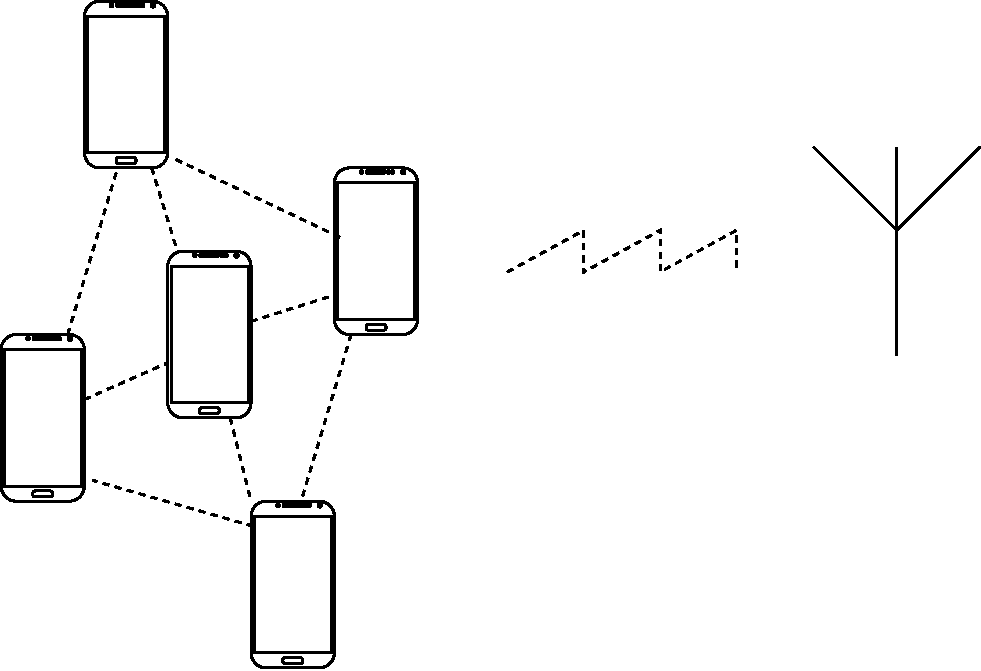
\includegraphics[width=0.8\textwidth]{images/context.pdf}}
	\caption{\label{fig:context} Example of an ad hoc network.}
\end{figure}

It is important to note that this work does not have the purpose of replacing the existing communication infrastructure, but is, in fact, trying to complement it.

\section{Objectives}
\label{sec:objectives}

This thesis will pursue two main objectives:

\begin{enumerate}
	\item 
	Developing a framework to create of a decentralized ad hoc network, where packets are transmitted between devices. Proving that, with the current unmodified Android versions and the Bluetooth technology, the creation of a network of that nature is feasible.
	
	To materialize the framework an application that implements this framework and exchanges web pages between devices is created. The application will create a solid ad hoc network. After the creation is complete the application will provide the logic to correctly manage the web pages request throughout the network, as well as their correct delivery. This application will then be submitted to a series of tests to comprehend where it is more vulnerable and where it is more robust.
	
	\item 
	The second objective will be to assess the advantages of migrating this application from Bluetooth to Wi-Fi Direct and what changes need to be made to the current Android versions to accommodate this migration. The advantages and disadvantages of Wi-Fi Direct in comparison to Bluetooth will be compared in the scope of the created framework. Conclusions will be drawn from a series of tests to compare both technologies. Also, a description of the obstacles, present in the current Android devices, preventing the development of this application using Wi-Fi Direct instead will be presented.
	
\end{enumerate}

This thesis will not provide a market product, thus it disregards some aspects of what would be to expect from a full consumer ready application. Security is not developed in this solution, although some ideas are given on how it can be provided.

\section{Contributions}

As mentioned before the created framework has a huge amount of possibilities. The purpose of this thesis is not to limit these possibilities to the transfer of web pages. It is to provide a simple to use developer kit that can be extended easily to exchange any message format, from web pages to beacon messages.

This is an open source framework and it is hosted in a GitHub repository\footnote{To download the code of the application clone the following repository: \url{https://github.com/Falcato/ThesisApp.git}.}. In here the full application code will be presented with the necessary comments to complement the description made in Chapter \ref{chapter:work}. By using the provided mechanisms developers can made the necessary modifications to the code in order to achieve different goals, \textit{e.g.} the creation of a peer-to-peer chat application.

Also, since the transfer of web pages is a complicated process and not much information is available on it, this application has a double usefulness, since it also demonstrates how to exchanges large files between devices.

A set of study tests on the advantages and disadvantages of Bluetooth and Wi-Fi Direct is presented in an easy and succinct fashion. Finally, several study tests on a not so common environment, a Bluetooth peer-to-peer application, are provided, revealing this technology's performance in an Android application.

\section{Structure of the Thesis}

The rest of this thesis is organized as follows:

\begin{itemize}
	
	\item Chapter \ref{chapter:soa} will begin with a theoretical introduction of the different wireless communication technologies, analysing their features, advantages and disadvantages. This aims to provide the needed background to understand the technologies used in this thesis and the choices made along its developments. There will be an analysis on the Android's implementation of Bluetooth and Wi-Fi Direct, as well as some of the possibilities it may present, such as ad hoc networking and multi-hop routing. Finally, an overview of some ad hoc networking applications in Android will be given, describing their features and technologies used.
	
	\item Chapter \ref{chapter:work} will contain the implementation of both framework and application. It will begin by a description of the steps taken to decide important parts of the framework, such as technologies and routing protocols used. The implemented network creation and communication protocols are explained, providing a better understanding of the framework. Lastly, the materialization of the framework, the peer-to-peer application to exchange web page is described, along with its features and overall packet exchanges.
	
	\item Chapter \ref{chapter:tests} will provide a theoretical and empiric evaluation of Bluetooth and Wi-Fi Direct, assessing how both technologies fare in certain aspects, useful for the proposed framework. Furthermore, several experiments will be performed on the developed application, in order to point its overall performance, strong and weak points.
	
	\item Chapter \ref{chapter:conclusion} will contain a final summary of what was developed and accomplish in this thesis will be presented. The possible future work to be developed in the proposed framework and application will be discussed. 
	
\end{itemize}









\chapter{State of the Art}
\label{chapter:soa}

\section{Communication Technologies Supported by Mobile Devices}
\label{sec:commtec}

\subsection{Mobile Networks Technologies}
\label{subsection:mobtec}

The first form of communication on mobile devices where the mobile cellular telecommunications provided by the Public Land Mobile Network. At first they did not have so many features as we know them now, they were limited to basic voice calls and short text messages. As devices became more sophisticated so did mobile networks, including new features, such as Internet connections and device to device communication.

Mobile networks have become common place, \textit{i.e.}, people make millions of phone calls and text messages everyday, using the service providers' \glspl{BS} to enter a network, where their message/phone call is being routed to its destination. This said, it is important in the scope of this work to have some understanding on how devices communicate with each other using these mobile communication standards.

In this subsection we will briefly present the existing standards for mobile cellular networks and their evolution, passing from 2G, 3G and 4G, emphasizing this last one.

\subsubsection{2G: GSM}

\gls{GSM} is a standard, created by European Telecommunication Standards Institute, to describe second generation cellular networks. These networks differ from the first generation due to the fact that they were no longer analog, as in 1G, and became digital, allowing for voice as well as text transfer.

\gls{GSM}'s architecture can be seen as hierarchical, with components ranging from \glspl{MS} to \glspl{MSC}. \glspl{MS}, the devices, have a unique number, with which a \gls{BS} can identify each one of the \glspl{MS} it controls. A \gls{BSC} controls multiple \glspl{BS} to allocate radio channels, manage call handover between \glspl{BS} and control their power levels, in order to avoid muffling the transmission of other \glspl{MS}. Finally, a \gls{MSC}, in charge of multiple \glspl{BS} connects to a Gateway \gls{MSC} where mobile registration and authentication are made.

\gls{GSM} uses the air interface to transfer information, being a wireless way of communication, specifically, it uses \gls{FDD}, to separate the uplink and downlink frequencies, 890-915MHz and 935-960MHz, respectively. Then divides each block of frequencies into smaller channels, 125 channels of 200kHz each, using \gls{FDMA}. In each \gls{FDMA} channel it's given a time slot for each \gls{MS} to use, using \gls{TDMA}. Using this methodology for medium access, \gls{GSM} allows for a data rate of 9.6kbps per user, after enctryption and error control overhead.

\gls{GSM}'s main technologies are voice communications, \gls{SIM} authentication, encryption and accounting information, handover, enabling \glspl{MS} to move and connect to a different \gls{BS} maintaining the service and SMS (Short Message Service), allowing for text transfer up to 160 characters, sent to one or multiple destinations.

In order to improve \gls{GSM}, \gls{GPRS} was introduced, also known as the 2.5G networks, adding two new elements to the previous \gls{GSM} architecture, a service support node for security, mobility and access control, a gateway support node for establishing connections to external packet switched networks. Although not much improvement on data rate was made on \gls{GPRS}, soon came \gls{EDGE}, which combined \gls{GPRS} with different modulations, improving the spectral efficiency of each channel and allowing for data rates up to 384kbps.

\gls{GSM} requires heavy resource planning, \textit{i.e.}, frequency and time planning and slot assignment, meaning each user has a dedicated time and frequency and thus the number of users in a cell does not influence the cell size.

\subsubsection{3G: UMTS}

\gls{UMTS} was the natural 3G evolution of the \gls{GSM}/\gls{GPRS} netowrk. It used the previously created \gls{GPRS} architecture and improved it using different \gls{MAC} techniques to improve even further spectral efficiency. The architecture of \gls{UMTS} is divided into radio access network, \gls{UTRAN}, in charge of managing cell-level mobility, and \gls{RNS} and air interface, \gls{UTRA}, similar to \gls{GPRS}. Now \gls{UTRAN} controls multiple \glspl{RNS}, who is responsible for handover decisions. The \gls{UMTS} network operates in parallel with the previously established \gls{GSM}/\gls{GPRS} network.

In \gls{UMTS} transmission is made over two 5MHz \gls{FDD} channels, using \gls{DSSS}, improving both the data rate and security of transmissions. \gls{W-CDMA} is now used instead of \gls{FDMA} and \gls{TDMA}, each user has a chipping sequence with which messages are encoded, in the destination, with the same chipping sequence the reverse process is made and the message is transmitted, allowing for similar data rates as \gls{EDGE} and users to transmit simultaneously with little interference, depending on the number of users.

\gls{UMTS} requires heavy power control, because the source can distinguish each user via their chipping sequences, but if one user muffles another user only one message is received in the destination, thus it is needed to control the power with which each user will transmit. This means the more users transmit simultaneously, more interference is created, assuming non ideal conditions, thus having to reduce cell size to compensate for this interference, leading to more complex cell planning.

In order to enchance the data rates of \gls{UMTS}, \gls{HSPA} was introduced, which is an evolution of \gls{W-CDMA}, 3.5G networks. This standard improved upling and downlink speeds, by adding higher-order modulation, \textit{e.g.}, 16QAM or 64QAM, and a more efficient retransmission mechanism in the downlink channel and by allowing parallel transmissions of multiple users, also known as \gls{MIMO}, reaching rates up to 168Mbps and 22Mbps, respectively.

\subsubsection{4G: LTE/LTE-A}

\gls{LTE}, came to meet the specified requirements in International Mobile Telecommunications-Advanced, issued by ITU-R. But since it did not meet all the requirements to be considered a 4G network, it was considered a 3.9G network. It introduced an exclusively IP-based packet-switching core network, denominated \gls{EPC}, and it targets the increase of quality of service, spectrum efficiency and reduced cost.

\gls{EPC} introduced new elements to the existing network, a Packet Data Network Gateway, serving as the termination of \gls{EPC} towards Internet, providing \gls{IP} services, address allocation, packet inspection and policy enforcement, a Mobility Management Entity, responsible for location tracking, paging, roaming and handover, and a Policy Charging Rules Function to manage the quality of service provided.

\gls{LTE} uses multiple frequency bands from 700MHz to 2600MHz, with a flexible bandwidth ranging from 1.4MHz to 20MHz, using both \gls{FDD}, \gls{TDD} and a combination of these two methods. This combined with \gls{OFDM} and \gls{MIMO}, for \gls{MAC}, allows \gls{LTE} to reach data rates of 326Mbps for downlink. In uplink a \gls{SC-FDMA} is used allowing for data rates up to 86Mbps. These data rates are considerably higher than the ones reached by \gls{UMTS}.

In order to further improve data rates on \gls{LTE}, \gls{LTE}-Advanced was introduced. This new network meets the requirements to be considered a 4G network, thus it is where 4G networks were actually introduced. Reaching up to 3Gbps for downlink and 1.5Gbps for uplink, Release 10, \gls{LTE}-Advance immensely improves data rates by using a much wider channel frequency and higher-order \gls{MIMO}, up to 100MHz, also improving on spectral efficiency.

A new type of networks is also introduced, the \glspl{HetNet}, created by deploying a low-power \gls{BS} at cell edges to enhance network perfomance. Three types of cells are created with this network: micro or pico cells, where a relay node is used to extend the service to other devices. Femto cells, for indoor coverage at home, offices or malls, where a Home eNodeB serves as relay node for devices inside the femto cell.

Considered for 4G \gls{LTE}-Advanced was the concept of D2D communications, creating direct links between devices within a small area. This technology would enable the linking of devices by using the cellular spectrum, allowing for data to be transferred from one to the other over short distances, but using a direct connection. This form of device to device has a lot of applications, \textit{e.g.}, in disaster scenarios, where the access to the infrastructure is denied, or when the infrastructure is overloaded in \textit{e.g.}, large public events.

4G \gls{LTE}-Advanced D2D was a feature in Release 12 and brought some benefits, such as reliable and persistent communication, meaning it persists if the \gls{LTE} network is disrupted, data rates, when the distance to an \gls{BS} is considerable and interference reduction, by not having to communicate directly with the \gls{BS} overloading the network. There are of course some issues to be addressed with this communication, such as the authorization and authentication of \glspl{MS} and the fact that inter-operator communication may not be approved by the different operators, limiting the possible links.













%!TEX root = ../dissertation.tex

\subsection{Wi-Fi (IEEE 802.11)}
\label{subsection:wifi}

A \gls{WLAN} is a wireless network that can connect multiple devices to each other within a limited range. \glspl{WLAN} have become very popular in the day to day life of people. Most households have a \gls{WLAN} deployed so that devices inside and around the premises can have Internet access. The popularity of \glspl{WLAN} is mainly due to the fact that devices do not need to be physically connected to the \gls{AP} to access the Internet, which removes the costs of cables and the associated infrastructures.

IEEE 802.11 is the \textit{de facto} standard for \glspl{WLAN} and it is commonly known as Wi-Fi. IEEE 802.11 is composed by \gls{MAC} layer and Physical layer specifications for \gls{WLAN} implementations, various versions have been released, but the most common are IEEE 802.11a/b/g/n/ac, mainly because they were adopted by mobile and computer manufacturers as the standard to be used in radio communication, \textit{i.e.} wireless.

Unfortunately, the connection speeds are not as high as in wired networks, since the environment plays a big role, \textit{i.e.} if there are obstacles between the \gls{AP} and devices. Also, the number of devices in the network will affect the data speeds, since the protocol specified for the IEEE 802.11 standard is \gls{CSMA/CA}. Although these are disadvantages over wired technologies, there has been done a lot of improvement on the data rates, during the development of wireless networks, reaching up to 6.93Gbps, using \gls{MIMO}, high-order \gls{OFDM} and enhanced \gls{MAC} techniques, see \cite{IEEE80211} for more information on this topic.

In \gls{CSMA/CA} the devices check the medium for clearance, \textit{i.e.} if there is no other device transmitting at that time. Nodes attempt to avoid collisions by transmitting the full data only when the medium is clear. Hidden node is still a problem with this \gls{MAC} method, meaning a node can be transmitting but its transmission is not detected by other devices, creating collisions.

In order to overcome the hidden node problem, \gls{RTS}/\gls{CTS} can be used to reserve the access to the shared medium. A control packet \gls{RTS} is sent by the transmitter, to which the receiver will answer with a \gls{CTS}. If the channel is clear the packet will be sent immediately, \textit{i.e.} if a \gls{CTS} was received, else the device will wait a random period of time, named backoff time, before checking if the medium is clear again. When the backoff timer reaches zero, the device will perform the check, if the medium is clear the device will send the packet, otherwise the backoff time is set again. Due to the exponential factor of this backoff time the connections' speeds are limited when multiple users use exhaustively the network channel, whereas in wired connections, like switched Ethernet, traffic management is, typically, done through traffic flow prioritization.

Another main consequence of establishing a \gls{WLAN} is the security of the communication. In wired networks there is a physical component to security, such as controlled access to the building. In \glspl{WLAN} networks this type of security is not relevant as, for instance, one can enter the network outside the building. Thus security protocols must be implemented to successfully prevent attacks on the communication between devices, such as WPA2 or IEEE 802.11i, see \cite{security} for more information on security protocols.

A \gls{WLAN} can have three different main modes of operation, infrastructure, ad hoc mode and Wi-Fi P2P. Besides these three main modes, IEEE 802.11s will also be briefly explained due to its characteristics and similarities with this work. In the next subsections these modes will be explained, and provided of pros and cons.

\subsubsection{Infrastructure}

Infrastructure is the most common method, usually deployed and made accessible by a local \gls{ISP} or by a Local Area Network. The structure of the network is as follows, there is a wireless \gls{AP} that manages the various devices on the network and provides the Internet access, this \gls{AP} can be either wired, \textit{e.g.} fiber, or wireless connected to network backbone. The \gls{AP} is responsible for the creation and maintenance of the network, it generates an SSID with which the network will be identified, aswell as a security level, \textit{e.g.} \gls{WPA} or \gls{WPS}.

\gls{MS}s can then connect to the network via wireless or wired connections. In the wired connections no authentication is required as there is a physical connection and usually higher data throughput is achieved. In wireless connections there is the need of first identifying the network to which the \gls{MS} wishes to connect and then to proceed according to the security level used by the \gls{AP}. The access to the network is managed by the \gls{AP}, the wired connections are, usually, granted priority over the network, whereas wireless connections compete for the usage of the air interface, typically, via a predefined \gls{MAC} protocol, being the most used \gls{CSMA/CA}.

An example of the infrastructure mode network layout can be seen in Figure \ref{fig:infranet}.

\begin{figure}[ht]
	\noindent\makebox[\textwidth]
    {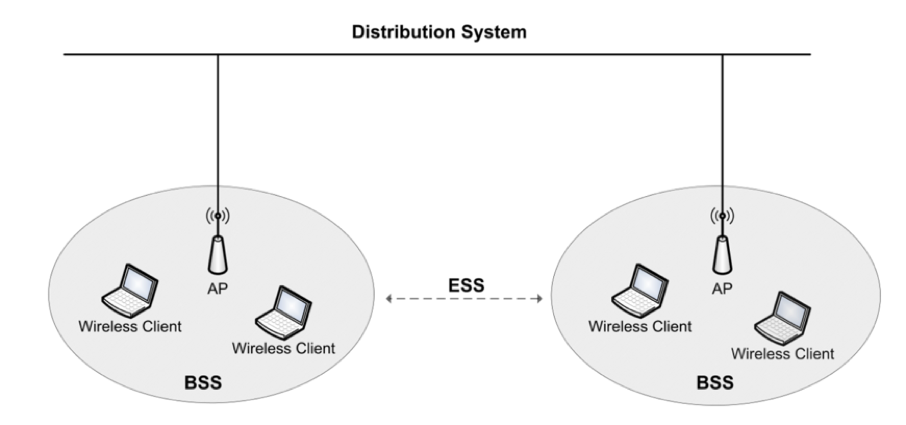
\includegraphics[width=1\textwidth]{images/infranet.png}}
	\caption{\label{fig:infranet} Infrastructure network layout (source: www.cse.wustl.edu)}
\end{figure}

Where each \gls{BSS} is a network and \gls{ESS} is a set of \glspl{BSS} that form a single sub network.

The infrastructure mode is ideal if the network as a more permanent character, since the \glspl{AP} are, usually, developed to provide higher-power wireless radios and antennas so that the area covered by the \glspl{AP} is wider. Despite being the most widely deployed method there are some disadvantages associated with this method, for instance, two \glspl{MS} will not be able to communicate directly even if they reside in the same network, and all their traffic is routed by the \gls{AP}, which brings another problem: in case of \gls{AP} failure due to, \textit{e.g.} power failure, software failure, \textit{etc.}, all the network will be compromised and to establish an Internet connection the \glspl{MS} will have to either connect to another \gls{AP} or to create the connection by themselves, which brings us to the next subsection.

\subsubsection{Ad hoc Networks}

In the ad hoc mode there is no need for a centralized \gls{AP}, meaning all the devices can connect to each other if within range. An ad hoc network is slightly different from a Wi-Fi Direct network (WIFI P2P) that will be described in the next section. In ad hoc mode the network is meshed, and all the devices within it are peers, which brings some benefits, \textit{e.g.} the direct communication between devices, without depending on a centralized point connected to the distribution system.

In ad hoc networks with a mesh topology there can be peer-to-peer exchange of traffic. This helps with the problem of having a centralized point of failure, such as the one present in infrastructure mode. Much like \textit{torrents} files can be transferred by smaller parts and by different providers, by using this method to transfer files, packets, \textit{etc.}, within the network higher data rates can be achieved, since multiple parts of the same file/packet can be sent simultaneously.

An example of the ad hoc mode network with a mesh topology can be seen in Figure \ref{fig:adhocnet}.

\begin{figure}[ht]
	\noindent\makebox[\textwidth]
    {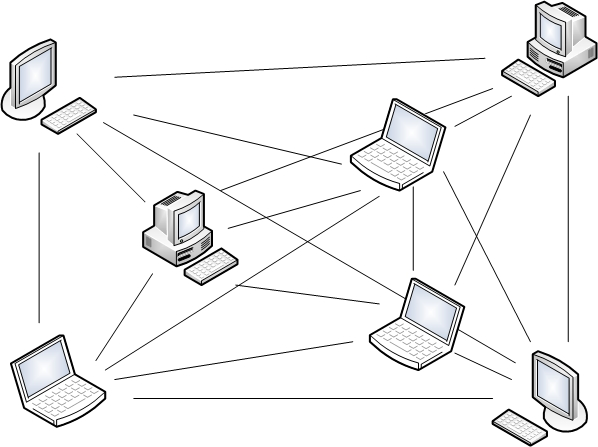
\includegraphics[width=0.5\textwidth]{images/adhocnet.jpg}}
	\caption{\label{fig:adhocnet} Ad hoc network layout (source: monet.postech.ac.kr)}
\end{figure}

As can be seen in Figure \ref{fig:adhocnet}, one device can have multiple links connecting him to other devices in the network. Although this is a big plus if compared with infrastructure mode, it must be noted that, as said before, a device can connect to other devices if in range, otherwise they will not be able to establish a link and thus communicate. This limitation is due to the lack of a routing protocol in this network mode, so nodes cannot serve as relay for communication between two \glspl{STA}, and although it is possible to implement a layer 3 (Network Layer) routing protocol with this mode, such as \gls{AODV}, it is not intrinsic to this mode. In the next subsection, IEEE 802.11s will be introduced and we will see that it covers this limitation of this ad hoc mode.

Although there are advantages such as not having a centralized point of failure, peer-to-peer file/packet transfer described above, there is an easier setup of the network and the problem described in the infrastructure mode of not existing a direct connection between two \glspl{STA} is now mitigated as every \gls{STA} in the network is a peer, there are some disadvantages associated with this network mode, such as the network being more dynamic which brings a lot of changes in the network topology, the interference inherent to all the devices transmitting at the same time to different peers and there is always the scalability problem as more devices in the network mean more connections, which grow exponentially, whereas in the infrastructure mode the connections grow only linearly, so ad hoc networks don't scale well. Also, due to the lack of a routing protocol, the range of the the network will be significantly reduced, as devices do not know which route to forward the packets, in order to reach a certain destination.

Furthermore, the network will not be able to reach the Internet, since devices will communicate between themselves and not with the infrastructure, making the packet exchange limited to the local/cached information stored in the devices, unless if the infrastructure and ad hoc networks are connected through a common device. Finally, the mobility of the devices can make the maintenance of stability of the network a difficult task as links may have to be created and destroyed regularly.

\subsubsection{IEEE 802.11s (Meshed Network)}

IEEE 802.11s is a standard introduced in 2011 which aimed to provide both broadcast and unicast delivery of information. The main difference between the previously described ad hoc mode is that IEEE 802.11s supports multi-hop and implements a layer 2 routing protocol named \gls{HWMP}.

In this standard, four main types of devices exist: \glspl{MP} who establishes peer links with other \glspl{MP}, \glspl{MAP} that is a characteristic of \glspl{MP} which provides \gls{BSS} services to support communication with \glspl{STA}, \glspl{STA} which are devices outside the meshed \gls{WLAN} and connect to the network via \gls{MAP}, finally, \gls{MPP} that is the point at which devices enter and exit the network.

\glspl{MP} discover potential neighbors based on beacon and probe messages, containing the \gls{WLAN} Mesh Capability Element, a summary of active protocols and other channel information, and the Mesh ID, that identifies the mesh. The devices are considered to be members of the network upon the establishment of a secure peer link with neighbors within the network. In Figure \ref{fig:ieee80211s}, taken from \cite{IEEE80211s}, it is possible to visualize an example of the network: 

\begin{figure}[ht]
	\noindent\makebox[\textwidth]
    {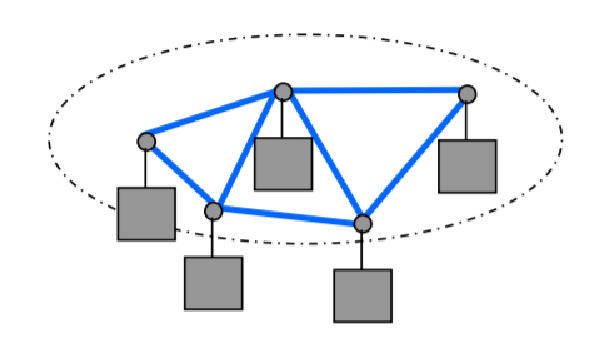
\includegraphics[width=0.7\textwidth]{images/ieee80211s.pdf}}
	\caption{\label{fig:ieee80211s} IEEE 802.11s network layout (source: \cite{IEEE80211s})}
\end{figure}

Depending on the number of radio interfaces the devices have, IEEE 802.11s allows for multi-group formation, where each radio interface of each device is assigned to a different group, called Unified Channel Graph.

The routing protocol used by IEEE 802.11s, \gls{HWMP}, is based on a combination of Radio Metric \gls{AODV} and tree-based routing, which provides great flexibility in changing environments, great efficiency in fixed mesh deployments, and possible extensibility to metrics other than simple number of hops, such as quality of service, load balancing and power-aware. With this features, \gls{HWMP} extinguished many of the ad hoc mode flaws, such as lack of routing protocol and thus inability to perform multi-hop transfer of packets and network range.

Although IEEE 802.11s comes with some benefits, pure ad hoc mode still predominates as the peer-to-peer mode, due to its simplicity. There are still some products that make use of the IEEE 802.11s, such as Linux operating system, FreeBSD operating system and Google WiFi routers.

\subsubsection{Wi-Fi Direct}
\label{subsection:wfd}

Wi-Fi Direct is a Wi-Fi standard created by Wi-Fi Alliance. The previously called Wi-Fi P2P, now Wi-Fi Direct, is an innovative way of mobile communication without the dependence of a physical AP. It can be used for different purposes, such as file transfer, Internet browsing, device communication, \textit{etc.}. Wi-Fi Direct assumes an ad hoc topology, meaning the devices are not dependent on one another, but form a network where all devices share information, hence called peer-to-peer. In Figure \ref{fig:wifidirnet}, it is possible to see the difference between traditional infrastructured Wi-Fi (to the right) and Wi-Fi Direct (to the left).

\begin{figure}[ht]
	\noindent\makebox[\textwidth]
    {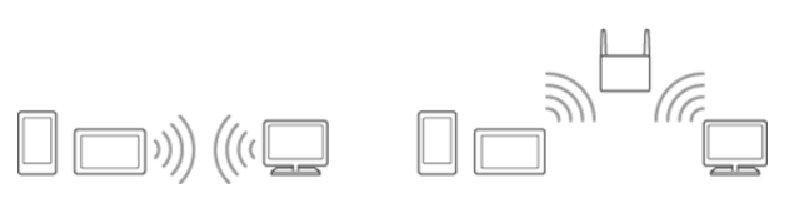
\includegraphics[width=0.7\textwidth]{images/wifidirnet.pdf}}
	\caption{\label{fig:wifidirnet} Wi-Fi Direct (left) and traditional Wi-Fi (right) network layouts (source: info.tvsideview.sony.net)}
\end{figure}

Wi-Fi Direct is not dependent on an infrastructure, meaning even without access to a Wi-Fi network it is possible for devices to connect with each other, this because the Wi-Fi Direct enables devices to emit a signal to other devices in the vicinity announcing the possibility of making a connection. Users in the vicinity of the sending device receive an invitation to join a network (Wi-Fi Direct group).

The process of group creation and administration is the most important topic to this work, regarding this technology. Devices can either join existing groups or create new groups, where they will be the administrators, \textit{a.k.a.} \glspl{GO} of that particular network. This type of creation forces the Wi-Fi Direct to shape its topology as a star, as is evidenced in Figure \ref{fig:wifidirnet}, where there is a central soft \gls{AP}. It is important to make clear the distinction between a soft and a physical \gls{AP}: the physical \gls{AP} usually refers to a physical router, that administrates a network with wired and/or wireless devices, whereas the soft \gls{AP} can be set up with a Wi-Fi adapter, present in many devices, such as mobile phones, computers, \textit{etc.}.

After the creation of a group, the \gls{GO} announces to all nearby devices its group, via the Service Discovery protocol, that sends a beacon packet with an \gls{SSID}, that will be the identifier of the network. Then, the receiving devices can connect to the desired network, by sending information about the device and what type of services it supports. Along with the unique identifier of that device, when received by the \gls{GO}, the devices become \glspl{GM} of that network, much like slaves in Bluetooth, see \ref{subsection:bt}.

In traditional Wi-Fi Direct, the connections are one-to-one or one-to-many, limiting the topology to a star topology, the purpose of this work is to migrate from that star topology to a more dense meshed topology where many-to-many connections are established, and the transfer of data is made faster and without as many relay nodes as in star topology.

The speeds of Wi-Fi Direct are similar to the ones in other Wi-Fi operating modes, reaching up to 250 Mbps. This is the main advantage of Wi-Fi Direct to its direct competitors, such as Bluetooth. As in other wireless technologies, the speed is affected by the environment where the network is inserted, the physical characteristics of the devices and the Wi-Fi physical layer they support, \textit{e.g.}, 802.11a, g or n.


\subsection{Bluetooth}
\label{subsection:bt}

A \gls{WPAN} is type of network where devices are connected wirelessly to each other, based on the standard IEEE 802.15. This definition seems to be quite similar to the one of \gls{WLAN}, but there is a considerable number of differences between the two. The term personal area network derives from the use that is to be given to such networks, in other words, \glspl{WPAN} are to be deployed in order to connect multiple devices of one's personal area, such as home, office, \textit{etc.}.

Bluetooth is one of the main technologies to implement a \gls{WPAN}, described above. It uses the 2.4GHz \gls{ISM} band, it was invented by phone company Ericsson, and is used to connect devices in a short range network.

Devices connect to each other forming \textit{piconets}, which is the term assigned to designate an ad hoc network formed by devices using Bluetooth. Each \textit{piconet} has a master, the device that controls the network, similarly to an \gls{AP} without providing access to the infrastructured network. Associated to each master there can be up to seven slaves, which are devices that take part in the same \textit{piconet}. Multiple \textit{piconets} can connect between themselves and form a \textit{scatternet}, as seen in Figure \ref{fig:bluetooth}:

\begin{figure}[ht]
	\noindent\makebox[\textwidth]
    {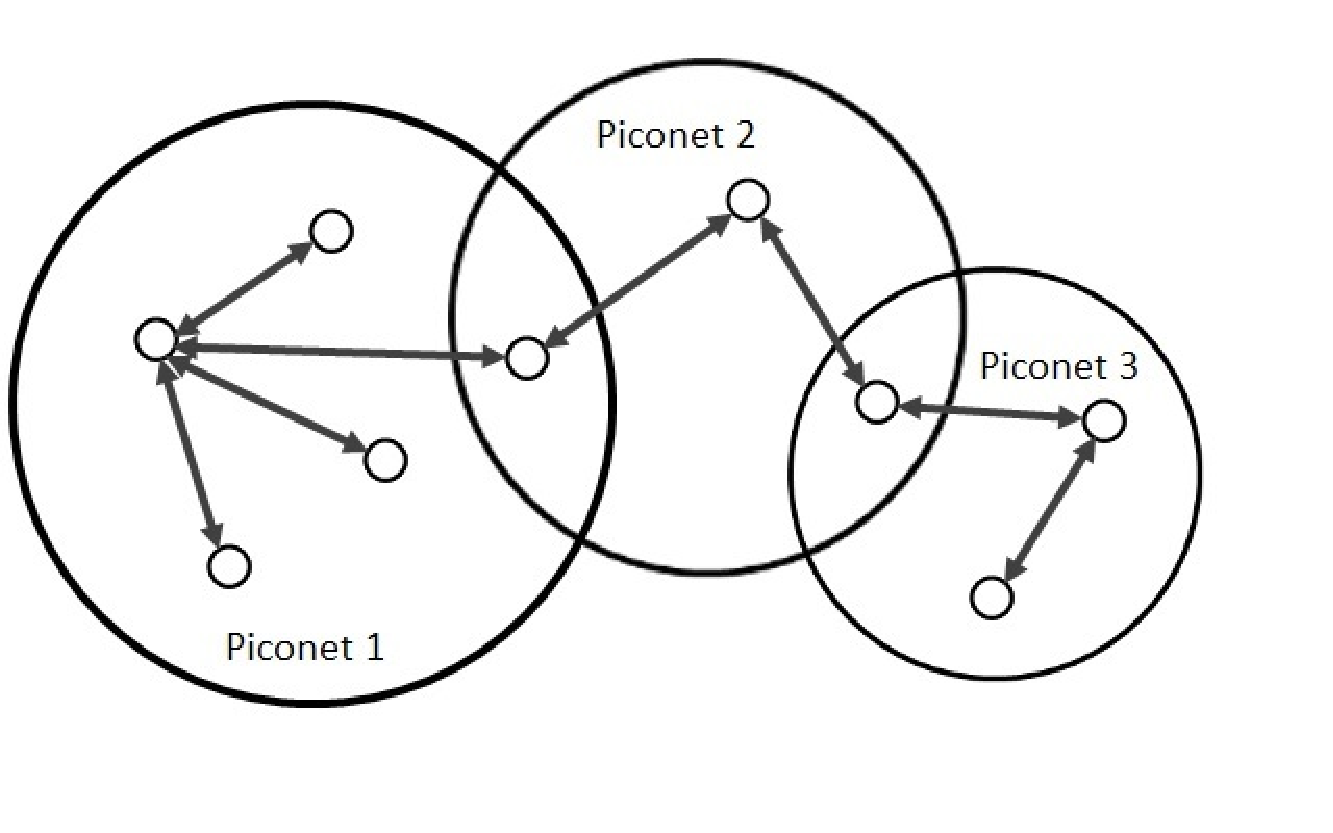
\includegraphics[scale=0.5]{images/bluetooth.pdf}}
	\caption{\label{fig:bluetooth} Scatternet Layout (adapted from: www.summitdata.com)}
\end{figure}

Each master is associated with a certain number of slaves, that can participate in more than one piconet, as seen above. These slaves are responsible for coordinating both \textit{piconets}, so that no interference exists.

Bluetooth uses slow \gls{FHSS} to control the frequency of transmission of each slave, this is done by creating a hopping sequence partially based on the master device's \gls{MAC} address, and then distributing the sequence to each slave on the \textit{piconet}. Devices connect to the \textit{piconet} by pairing with the master, forming a secure link, the master then controls the access to the medium by deciding which slave will transmit at a certain moment in time. In the \textit{scatternet} case, the data to be transmitted from \textit{piconet} to \textit{piconet} is relayed by the node participating in both networks. The pairing of both \textit{piconets} is similar to the pairing of a master and a new member of the network.

Although several advantages of Bluetooth are clear, such as low power wireless protocol, low transmission headers, ease of set up, multi group information transfer, this protocol still has a lot of downsides. The main current problems with Bluetooth consist in the low range of connections, due to the week signal power being a feature of the technology, the limited number of users that can form a \textit{piconet}, due to the narrow band used by Bluetooth and, finally, the low data rates of the protocol, which are heavily surpassed by the Wi-Fi standard.

\gls{WPAN} uses, typically, technologies that allow communication between devices within a certain specific range, usually around 10 meters, making this type of network much smaller than the ones created by \gls{WLAN}. The most common technology is Bluetooth, although there are several other technologies that are beginning to raise awareness, due to the crescent interest taken in \gls{IoT}, such as ZigBee. The used radio band is the 2.4 GHz \gls{ISM} band, due to its general availability worldwide and its lower cost.

\gls{BLE} is the power-version of Bluetooth developed for \gls{IoT}. The natural power-efficiency of Bluetooth combined with lower energy consumption provides the key factors for devices running for long periods of time without recharging. \gls{BLE}'s key features include: standard wireless protocol, allowing for interoperability across platforms, low idle power consumption and data encryption for security of communications, among others.

\gls{BLE} achieves data rates similar to classic Bluetooth over the same distance, although the application throughputs are much smaller: 0.27Mbps compared to 0.7-2.1Mbps for classic Bluetooth. The spectrum range of \gls{BLE} is the same as in classic Bluetooth, but the channels are two times wider than in Classic, consequently, there is half the number of channels. The main difference between the two lies in the power consumption and peak current consumption, 0.01-0.5W and less than 15mA for \gls{BLE}, 1W and less than 30mA for classic Bluetooth. The number of slaves in \gls{BLE} is implementation dependent as opposed to the fixed seven in classic Bluetooth.

\gls{BLE} is appropriate for networks that rely on the longevity of the battery of the devices, application throughputs are smaller but the information to be sent is, usually, also much less than in classic Bluetooth. One of the biggest limitation of \gls{BLE} is the inability to transmit voice, whereas classic Bluetooth is able. Despite this and other disadvantages of \gls{BLE} there are many areas that can benefit from technologies such as this one, \textit{e.g.} healthcare applications, logistic sensors, sports, among others, so it is not a technology that should be overlooked.












\subsection{NFC (Near Field Communication)}
\label{subsection:nfc}

\gls{NFC} is a short-range high frequency wireless communication technology that allows data transfer between devices over small distances, first introduced by three manufacturers, Sony, Nokia and Philips. Communications maintain interoperability between other different communication methods, such as Bluetooth.

\gls{NFC} can be used to connect mobile applications with the physical world, \textit{e.g.} home appliances, connect devices through physical proximity, forming a peer-to-peer network, and card emulation, creating a connection to a common infrastructure and allowing some actions on the infrastructure, such as making payments.

Evolved from \gls{RFID} technology, an \gls{NFC} chip operates as one part of a wireless link. Once it is activated by another chip, small amounts of data can be exchanged between the pair if within a few centimeters from each other. One of the advantages, compared to other wireless communication technologies, is that \gls{NFC} does not requires a setup to pair two devices, thus reducing the time and packets exchanged in the transaction, allowing for times up to 1ms. Also, \gls{NFC} chips run on low amounts of power, making this technology much more power-efficient than other technologies.

The short range of the \gls{NFC} technology is a disadvantage due to its spacial limitation, but in terms of security, this spacial requirement provides a higher degree of security than Bluetooth. For instance, making \gls{NFC} relatively secure to use in crowded areas, where other wireless technologies could be impossible to use to transfer sensitive data, such as credit card data.

\gls{NFC} operates at 13.56MHz using Amplitude Shift Keying as the modulation scheme and \gls{TDD} for simultaneous receive and transfer of data, achieving data rates up to 424kbps, and although these rates are not impressive, for the amount of data that is sought to exchange using this technology and the lack of necessity for communication setup, \gls{NFC} provides relatively fast transfer times.







\subsection{Conclusion}

Mobile network technologies have been improving at a fast pace, since the demand for higher speeds is constant. With the evolution of modulation methods to higher-orders and \gls{MAC} protocols improving spectrum efficiency and number of users in the network without interference, the demand for higher speeds has been successfully answered. 5G networks should focus further on resource optimization and a massively distributed \gls{MIMO} system.

Wi-Fi technology has many different standards, some being the natural evolution of the others, some serving different purposes, such as IEEE 802.11s. The Wi-Fi infrastructure mode has been constantly updated with better \gls{MAC} and modulation techniques, allowing for higher data rates and more users on the network. Ad hoc networks have also been evolving being the best candidate to offload some of the traffic in the infrastructure mode, also to achieve smaller, independent networks. Wi-Fi Direct has appeared as a possible method to implement ad hoc networks. Its support is still limited in devices, only allowing for some of the features it can provide. Progresses must be made in order to utilize this technology to its full capabilities.

Bluetooth has had a similar development to the IEEE 802.11 standard, evolving to faster data rates from version to version. Used for smaller networks than Wi-Fi, Bluetooth is widely used to deploy \glspl{WPAN}, now with the concurrence of Wi-Fi Direct, although they can both be used simultaneously. \gls{BLE} was also a big development in low energy networks, allowing for fast data transfer with low power consumption. Each Bluetooth technology has its utility, and the future focus should be in expanding the number of allowed users and range of the networks.

Finally, \gls{NFC} provides technology for yet another type of network. This time with a range even smaller than \glspl{WPAN}. It has a lot of applications but it's widely known for its easy and secure usability in transactions. It is being researched by industry giants like Amazon and AliBaba, but there is still much room for improvement, in security, network range, data rates, \textit{etc.}.

Overall we can say that most technologies have met huge improvements in short periods of time, and the tendency is to continue that way. Data rates will continue to grow as higher-level modulation techniques are discovered and new \gls{MAC} protocols are proposed. More emphasis has been given to smaller device to device networks in later years, has a way to take some load from the infrastructure, or even to for networks relevant to day to day tasks (\gls{IoT}).








%TEX root = ../dissertation.tex

\section{Wi-Fi Direct in Android}
\label{sec:wfd}

In this section, the current Wi-Fi Direct Android implementation will be described and analysed. There are small differences depending on the operating systems in which Wi-Fi Direct is being implemented, thus it is not possible to universally describe Wi-Fi Direct with more detail than the one used in Subsection \ref{subsection:wfd}.

In the next subsections, the details intrinsic to the Android operating system will be introduced and explained, followed by an in-depth description of various works on how to improve and expand the functionalities of this implementation.

\subsection{Wi-Fi Direct Star Formation}
\label{subsection:wfdstar}

As previously mentioned in Subsection \ref{subsection:wfd}, an ad hoc network is implemented in Wi-Fi Direct, by using a protocol for discovery and connection of the \gls{GO} with the \glspl{GM}. The \gls{GO} functions as a typical Wi-Fi \gls{AP}, managing the different communications of the \glspl{GM}.

\glspl{GO} are not predefined. It is during the group creation that the actual \gls{GO} is chosen, according to the specified parameters of the protocol, \textit{e.g.} battery percentage. This feature is relevant to manage the vitality of the network as a mesh of groups, since the \glspl{GO} can be chosen dynamically extending the life of the network.

After the process of the group creation, the \gls{GO} periodically sends a beacon to advertise the group, enabling other devices to discover and join the group. This advertisement is made in two different ways, either via Wi-Fi Direct, or via typical Wi-Fi. In the first way, devices discover the network via the Wi-Fi Direct discovery protocol, and join using the described set of actions. In the second way, the \gls{GO} announces the \gls{SSID} of the network and other devices, also known as legacy clients, connect via infrastructure mode Wi-Fi, using the \gls{SSID} and password, if set, to identify the \gls{GO}'s network. This leaves us with two different types of clients: legacy and normal. This differentiation will be the key to overcome the lack of multi-group interaction.

In Android devices, \gls{IP} addresses are predefined according to the function the device performs within the network. The \glspl{GO} are automatically assigned the following \gls{IP} address: 192.168.49.1/24, using \gls{DHCP}. Whenever a P2P or legacy client connects to the group, \gls{DHCP} is run again and the clients take an \gls{IP} address ranging from 192.168.49.2/24 to 192.168.49.254/24, chosen randomly to minimize the chance of conflicts. The \glspl{GO} are always assigned the same \gls{IP} addresses, unless they participate in another group as a \gls{GM} taking the same \gls{IP} as a regular client - see \cite{routeMultiGroup} for a more detailed explanation on this topic.

This technology is still not implemented to the best of its capacity in Android devices. The lack of a routing protocol that can establish multi-group communication, establishing a meshed network is an essential tool to achieve ad hoc networks. The current state of this technology in Android devices is a single group network with one-to-many links established from the \gls{GO} to the \glspl{GM}, which limits both the range and scalability of the network. Wi-Fi Alliance states that it is possible to overcome these limitations using stock devices, by creating software to allow for multi-group formation, although it is not standardized in Android's current version 7.0 "Nougat".

In the next section, a collection of developed work will be presented where the different authors propose different methodologies to overcome the lack of this feature in Android devices.

\subsection{Ad Hoc Networking}
\label{subsection:adhocnet}

C. Casetti \textit{et al.} propose in \cite{routeMultiGroup} a process to successfully form a meshed network, by allowing multiple groups to communicate. This proposition is based on stock Android, not requiring any "root" to be made to the devices, meaning all the actions will be performed in application layer, not envolving any changes in \gls{IP} addresses or \gls{MAC} interfaces.

The authors state that multi-group formation can be implemented by taking advantage of both virtual network interfaces of a device, \textit{i.e.}, the Wi-Fi or legacy interface and the Wi-Fi P2P interface, using each one to act as bridge in each group.

This said, upon experimentation, the following scenarios are not feasible in stock Android, due to the inability of creating a custom virtual network:

\begin{itemize}
\item a device is the \gls{GO} of one group and \gls{GM} in another,
\item a devices is the \gls{GO} of two or more groups,
\item a devices is a \gls{GM} in two or more groups (non-legacy).
\end{itemize}

Due to these limitations, the authors propose that a \gls{GO} be a legacy client in a different group, seen in Figure \ref{fig:mgrouprouting}:

\begin{figure}[ht]
	\noindent\makebox[\textwidth]
    {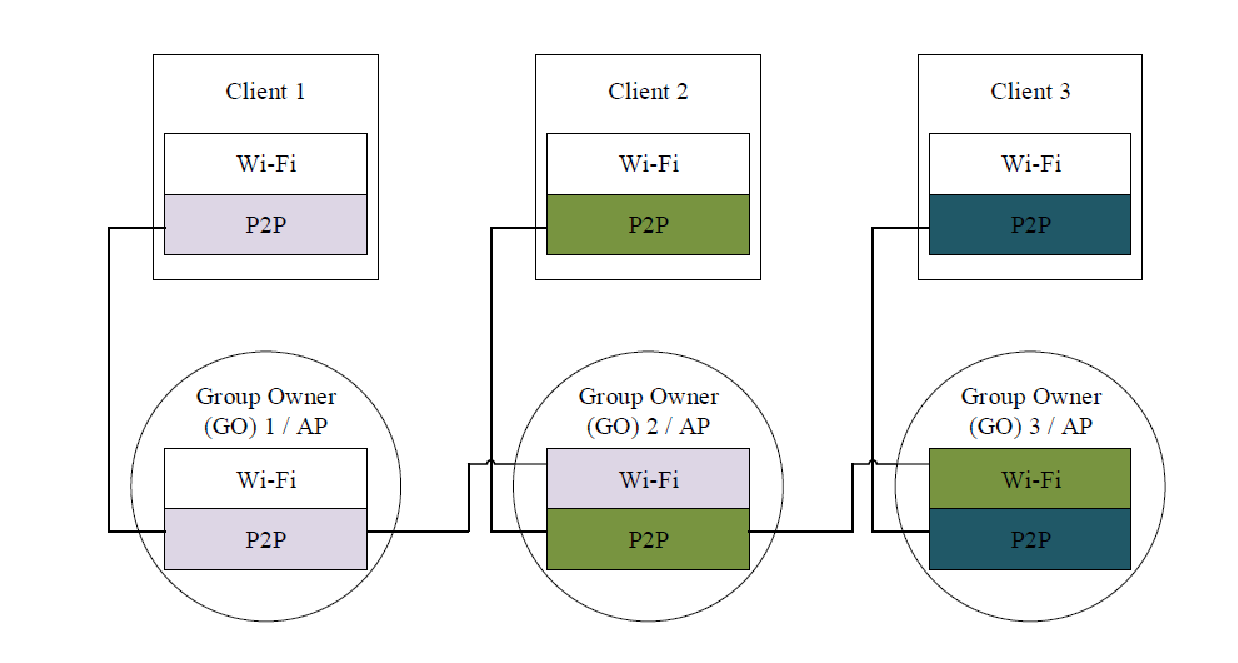
\includegraphics[width=1\textwidth]{images/mgrouprouting.pdf}}
	\caption{\label{fig:mgrouprouting} Multi-group physical topology with six devices (source: \cite{routeMultiGroup})}
\end{figure}

So, for each \gls{GO} two network interfaces are enabled, one is the conventional Wi-Fi and the other used for Wi-Fi Direct connection. The \gls{IP} addresses are assigned according to the previous description.

Two cases are distinguished by the authors: the \gls{GO} is not connected to any other group as a legacy client, which is the default topology of the network. In this case all connections are feasible, as Wi-Fi Direct has been implemented in order to provide full connectivity among all devices of a single group.

In the second case, the \gls{GO} is connected to another group as a legacy client as depicted in Figure \ref{fig:mgrouprouting} Groups 2 and 3, limiting data transfer to only a subset of D2D data. These limitation are due to two reasons, first the \gls{IP} conflict of both \glspl{GO}, who share the same address, 192.168.49.1, making the communication between two adjacent \glspl{GO} impossible. Secondly, when a \gls{GO} wants to send a unicast packet to any client, the packet is sent through the \gls{GO}'s Wi-Fi interface, due to Android's implementation of routing table entries in the \gls{GO}.

So in this case, client-to-\gls{GO} communication is allowed since client routing tables list only one interface and there are no conflicts, in \gls{GO}-to-client direction, bidirectional unicast communication is not allowed. Broadcast communication on the other hand is possible, since it is always sent through the \gls{GO}'s P2P interface. Although when they reach the \gls{GO} acting as a legacy client they are dropped due to the \gls{IP} address conflict mentioned above. Finally, client-to-client communication is bidirectional and sent through the client's P2P interface.

It is known from the first case that full connectivity among devices in a single group is allowed, even if one of the \glspl{GM} is a legacy client and \gls{GO} of another group. Based on this, the authors introduce the term relay node, which is used to describe this legacy client. The relay node is used to connect two groups. This node is chosen at random, upon the sending of a message from the \gls{GO} to one of its clients  chosen at random among those who do not act as \gls{GO} in another group. It is important to note that the authors state that this message must be broadcasted to avoid sending it through the Wi-Fi interface, the problem described above in the second case. These clients provide the communication backbone and provide connectivity to all other clients in the group, except from the ones acting as \glspl{GO} in another group.

\begin{figure}[ht]
	\noindent\makebox[\textwidth]
    {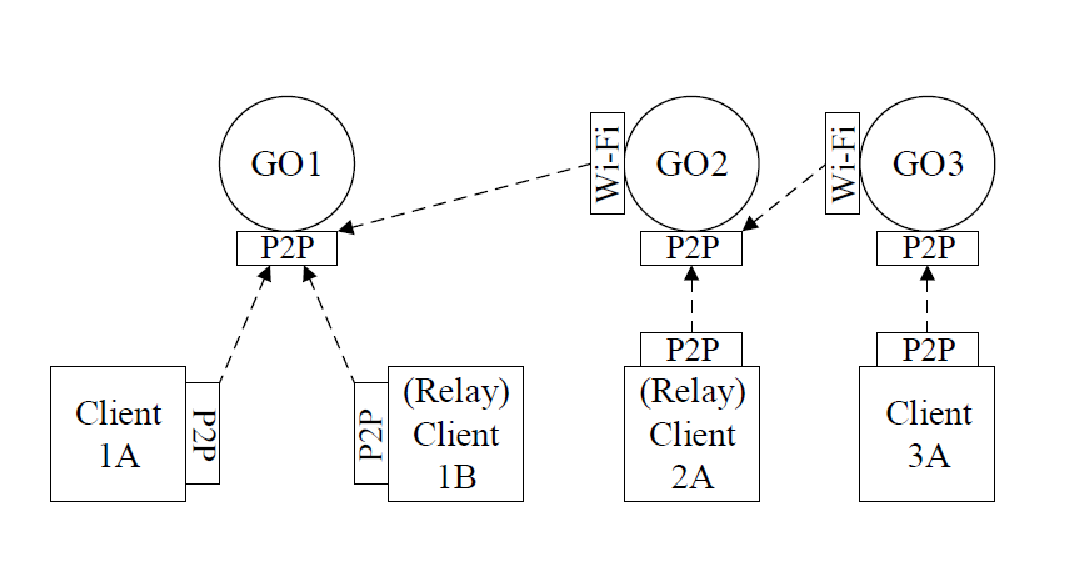
\includegraphics[width=0.9\textwidth]{images/1o1routingMGroup.pdf}}
	\caption{\label{fig:1o1routing} Example network topology with 3 Wi-Fi Direct groups. (source: \cite{routeMultiGroup})}
\end{figure}

Take Figure \ref{fig:1o1routing}, where only Wi-Fi Direct connections are represented, for instance. The procedure for Client 1A to send a packet to Client 3A is as follows: Client 1A encapsulates the data in the payload of a unicast \gls{UDP} packet and sends it to the relay Client 1B. The packet will be forwarded by GO1 to Client 1B, at the \gls{MAC} layer.

The packet is processed at the application layer and the payload is duplicated into a new \gls{UDP} packet. Sent directly to GO2's standard Wi-Fi interface \gls{IP} address. At the \gls{MAC} layer, the packet is sent to GO1, which sends the packet to GO2, via Wi-Fi direct.

The same process is repeated by GO2, but the packet is sent as a broadcast \gls{IP} packet through GO2's Wi-Fi Direct interface, to relay Client 2A. This client replicates the process of relay Client 1B, sending it to the \gls{IP} address of GO3's Wi-Fi interface.

Finally, GO3 processes the received packet and sends it to its destination with the correct payload, broadcasting it, similarly to the procedure of GO2.

This mechanism is used following the second case, where the \gls{GO} is connected to another group as a legacy client. With this mechanism the packet is successfully sent from group to group until its destination is reached, using a mix of unicast and broadcast communication.\newline

C. Funai \textit{et al.} propose a similar approach in \cite{multiHopD2D}. Their approach is to test two distinct possibilities for multi-group formation, as seen in Figures \ref{fig:mhopd2dgm} and \ref{fig:mhopd2dgo}, where "LC" stands for legacy client and refers to clients that use the classic Wi-Fi interface, instead of the P2P interface to connect to a group.

\begin{figure}[ht]
	\noindent\makebox[\textwidth]
    {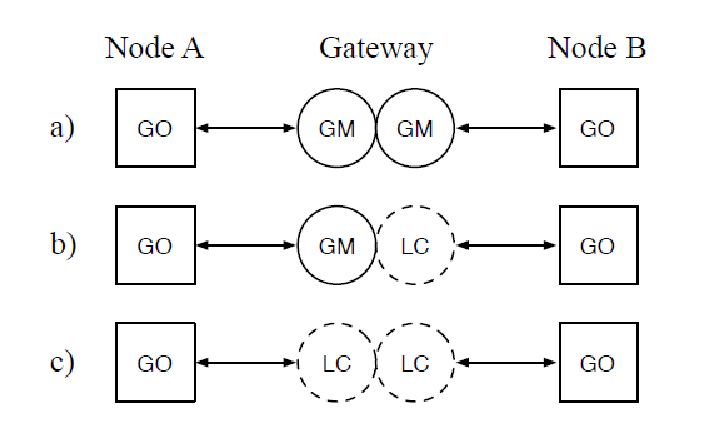
\includegraphics[width=0.6\textwidth]{images/mhop2d2GM.pdf}}
	\caption{\label{fig:mhopd2dgm} Multi-group communication scenarios where the gateway node acts as a client in two groups (source: \cite{multiHopD2D})}
\end{figure}
\begin{figure}[ht]
	\noindent\makebox[\textwidth]
    {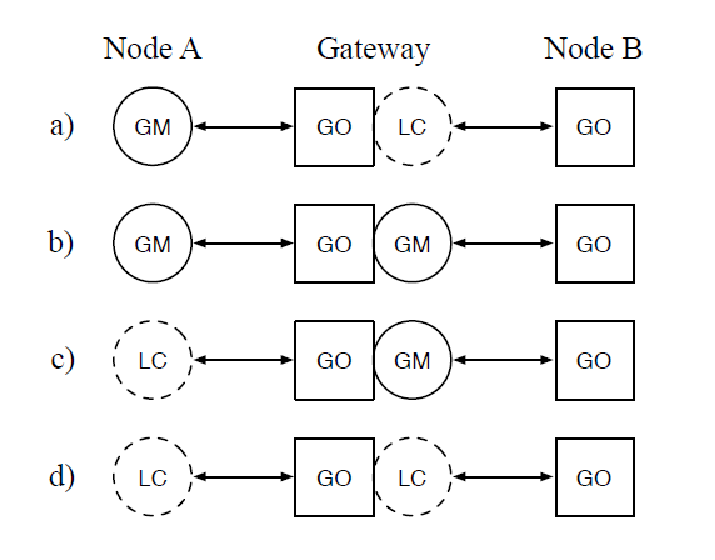
\includegraphics[width=0.6\textwidth]{images/mhop2d2GO.pdf}}
	\caption{\label{fig:mhopd2dgo} Multi-group communication scenarios where the gateway node acts as the GO in one group and as a client in the other (source: \cite{multiHopD2D})}
\end{figure}

The term gateway node is introduced, referring to the device that connects multiple groups. First by iteratively switching between the different P2P groups, relaying data between them. Secondly by using \gls{UDP}-based broadcast and a \gls{UDP}/\gls{TCP} hybrid solution to achieve multi-group communication. And finally by modifying the source code of the Android operating system.

The authors describe the limitations of stock Android, one of which the multi-group communication must be handled at the application layer and not at the network layer. Actions such as setting \gls{IP} addresses and managing routing tables cannot be performed without reprogramming the operating system of the device. Another limitation, already referred in \cite{routeMultiGroup}, is the inability to create virtual network interfaces or multiple virtual MAC entities.

These limitation result in the failure of direct implementation of the test scenarios shown in the figures above. Despite this, the authors state that it is possible to use Wi-Fi Direct functionalities simultaneously with an infrastructure wireless network, reaching the conclusion that the operating system is creating a virtual network interface. But the same interface cannot be connected simultaneously to multiple groups. Thus, scenarios \textit{a)} and \textit{c)} from Figure \ref{fig:mhopd2dgm} and scenarios \textit{b)} and \textit{c)} from Figure \ref{fig:mhopd2dgo} are not feasible using simple application layer procedures.

Although it is possible to use both interfaces concurrently and the connection between the groups is successfully established, the experiments from the authors suggest that it is not possible to create a unicast communication to and from the gateway node. For scenario \textit{b)} of Figure \ref{fig:mhopd2dgm} the gateway node was able to receive data from both groups but was not able to send. For scenario \textit{a)} and \textit{d)} of Figure \ref{fig:mhopd2dgo} the gateway node was able to communicate with node A but there was no communication with node B. The authors believe this is due to the fact that the \gls{DHCP} protocol assigns the same \gls{IP} address to multiple \glspl{GO}, creating a routing problem, also referred by C. Casetti \textit{et al.} in \cite{routeMultiGroup}.

Three solutions to this problem are presented: the first is time sharing, which will allow the implementation of any scenario in the figures above. In this solution, the gateway node is alternatively connecting between groups, \textit{i.e.} disconnecting from the current group, scanning for active devices and request to connect to the new group. In the scenarios of Figure \ref{fig:mhopd2dgm} the gateway node acts as client in both groups, thus neither group has to be destroyed for this switch to occur. Alternatively, in the scenarios of Figure \ref{fig:mhopd2dgo} one of the groups has to be destroyed, since the gateway node acts as owner for one group and client for the other. The main difference between the different scenarios within each figure is the protocols used to connect and disconnect to a group, \textit{i.e.} Wi-Fi Direct, classic Wi-Fi or a hybrid combination of the two.

A different solution proposed by the authors would allow simultaneous connections between groups. This can only be achieved by using a hybrid combination of the protocol, as already discussed, so only some scenarios will be tested. The authors tested the different topologies with different network sockets, \textit{e.g.} stream, datagram and multicast sockets. These tests showed that when combining a LC/GM, or \textit{vice-versa}, with a multicast socket, the gateway node is able to communicate with both groups simultaneously. Although the multicast socket only encapsulates one-to-many unicast communication, underutilizing the bandwidth of both protocols.

From the authors' experiments, the gateway node is able to receive and send data over the standard Wi-Fi link, while being connected to both groups with a unicast socket. But no data can be routed with the unicast socket over the P2P link. The reason for this is that Android  prioritizes standard Wi-Fi links over P2P links. So the \textit{Hybrid} protocol is proposed, where the multicast socket acts as a control channel to change the configuration of the gateway node. The gateway node receives a control message from a \gls{GM}, it then verifies which type of link it established with the group. In case of a standard Wi-Fi link, the node starts the reception of the data and disconnects from the same group after the reception is finished, creating a \gls{TCP} connection with the other group to send the data. In the second case, the node is not allowed to receive data, so a notification message is dispatched and the node disconnects from both groups re-connecting with the correct configuration, \textit{i.e.} inverting the link types.

Finally, the authors modified the source code of Android 4.4.2, altering the current implementation of Wi-Fi Direct to assign a unique \gls{IP} address to each \gls{GO}, mitigating the routing problem. This allows for a gateway node that uses both interfaces, and acts as \gls{GO} in one group and as a legacy client in the other.\newline

A. Shahin \textit{et al.} propose an Efficient Multi-group formation and Communication (EMC) protocol for Wi-Fi Direct, in \cite{emc}. This protocol allows multi-group formation as the solutions presented before, only this time the protocol has some significant improvements. EMC exploits the battery conditions of the devices in the network to select the \glspl{GO} of each group and enables the dynamic formation of Wi-Fi Direct groups. With these features EMC is a very efficient protocol if battery is an essential resource, \textit{e.g.} during an emergency period.

The authors utilized Wi-Fi Direct's service discovery feature to allow devices wishing to form a group to share information on their battery status. The algorithm will then choose the device with a richer energy reserve and elect it as the \gls{GO}. The rest of the devices can then connect to the created group as \gls{GM}. Some of these \glspl{GM} are referred as \glspl{PM} and are the \glspl{GM} that link a group to another, similar to the definition of bridge and gateway nodes introduced by the other authors. \glspl{PM} use their standard Wi-Fi interface to join another group, as a legacy client, forming a network topology similar to the one in Figure \ref{fig:emc}.

\begin{figure}[ht]
	\noindent\makebox[\textwidth]
    {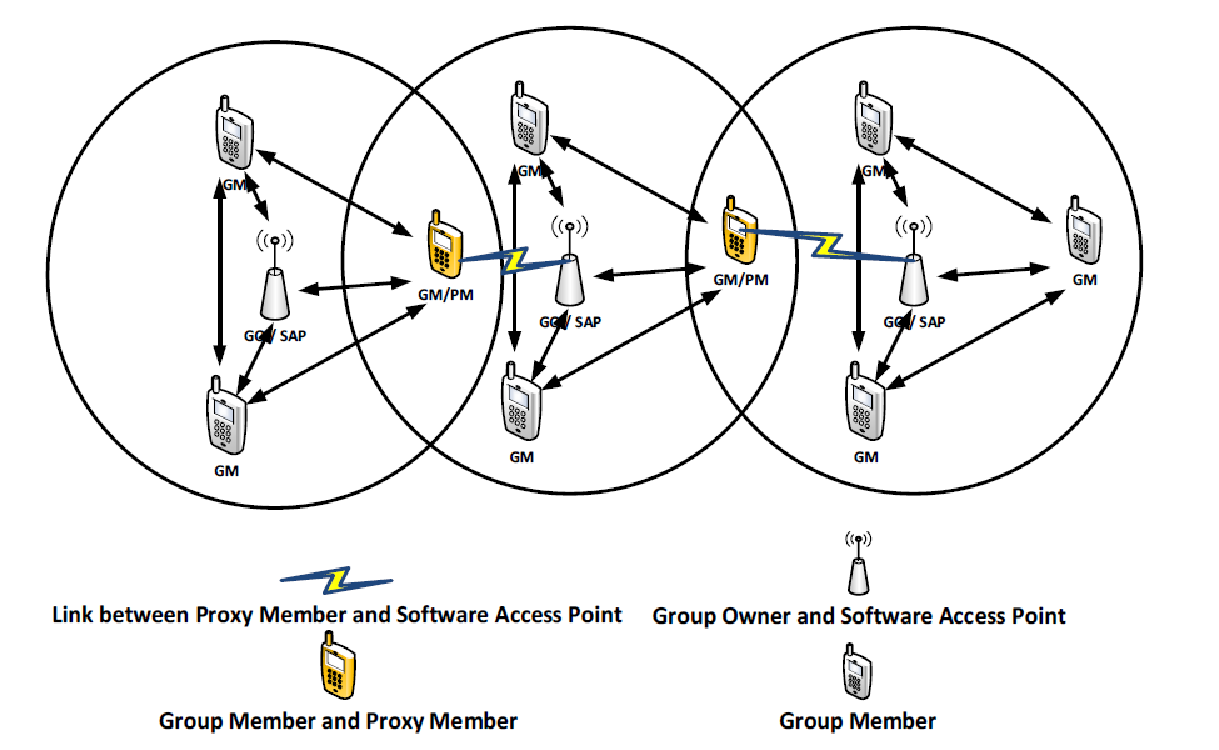
\includegraphics[width=1\textwidth]{images/emc.pdf}}
	\caption{\label{fig:emc} Example of a network topology after running EMC (source: \cite{emc})}
\end{figure}

After the group is created and \gls{PM} selected, the \gls{GO} waits for a period of time before tearing down the group and restarting the EMC protocol. This is done to ensure that the battery drain of the \gls{GO} is minimal and that groups can be established with all the devices for the maximum period of time. Upon restart, the new \gls{GO} is elected and the process is repeated.

In order to overcome the limitations of stock Android already discussed, the authors decided to modify Android's source code. By doing this, multi-group bidirectional unicast communication is allowed. Also, the issue of \gls{IP} addresses assignment is mitigated by giving \glspl{GO} different addresses.

Finally, in order to validate the protocol the authors created a chat application, which runs autonomously without any user interaction, apart from the messages to be sent. Manual override buttons are also present in the application for users to manually control the group creation and teardown.\newline

K. Liu \textit{et al.} propose a new implementation of \gls{MANET}
 using Wi-Fi Direct in stock Android, in \cite{manet}. It is the authors' belief that \glspl{MANET} using this technology can be used in \gls{LTE} offloading systems. This implementation has the following properties:

\begin{itemize}
\item All devices must have the same setup, \textit{i.e.} same functionalities.
\item The devices must be ready to be discovered, connected and to transmit
\item The \gls{MANET} is dynamic so devices must be able to join different groups in the network
\item All devices are able to leave or join the network, making the \gls{MANET} not depend on any device
\end{itemize}

This solution follows a different approach than the previously presented. According to the authors, in order to achieve all of the properties listed above, all devices must become \glspl{GO} when there is no data transmissions, creating a topology similar as the one in Figure \ref{fig:manettop}.

\begin{figure}[ht]
	\noindent\makebox[\textwidth]
    {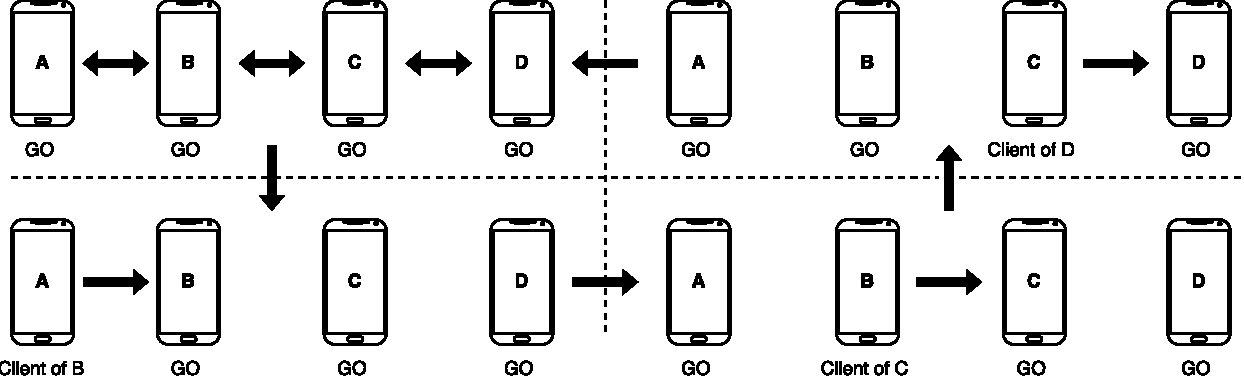
\includegraphics[width=1\textwidth]{images/manettop.pdf}}
	\caption{\label{fig:manettop} Wi-Fi Direct MANET topology (adapted from: \cite{manet})}
\end{figure}

The transmission cycle is as follows: the device with data to transmit must first remove its \gls{GO} status and connect to the destination as \gls{GM}, via the Wi-Fi Direct interface. Once the connection is established, the devices may communicate between them. After the transmission, the device acting as a \gls{GM} disconnects from the group and becomes a \gls{GO} again. This cycle is repeated whenever there is data to transmit.

This \gls{MANET} topology is implemented in stock Android devices, as previously mentioned, and presents a distinct solution from the other works, since the devices in the network are constantly changing roles and groups inside the \gls{MANET}. One disadvantage of this solution is that the status change of the devices are triggered by human interaction with the application, making the network somewhat dependent on human interaction.

\subsection{Multi-Hop Routing}
\label{subsection:mhoprouting}

In the previous section some methods proposed by different authors were presented, in order to create a multi-group networks using Wi-Fi Direct. In this section the focus will be the routing algorithms implemented over some of these methods.

In \cite{routeMultiGroup}, C. Casetti \textit{et al.} propose a content-centric routing algorithm on top of the network topology proposed. Meaning each node knows what is the next hop to which it has to send the request for a specific content - see \cite{contentcentric} for a detailed explanation on content-centric networks.

The authors introduce two data structures responsible for storing the information for content routing: \glspl{CRT}, providing the next hops to reach a certain content. These tables function similarly to standard \gls{IP} routing tables. They store the MD5 hash of the \gls{IP} address of the next hop.

There are three possible scenarios for filling the \gls{CRT}:
\begin{itemize}
\item The simplest one where the content item is available within the group of the content requester, where the next hops of the all \glspl{GM} is the \gls{IP} address of the content provider.

\item The second scenario is when the content is available in a different group, reachable through the group's relay node. This means the \gls{GO} of the second group is connected as a legacy client to the first group and, according to the authors' scheme, all the \glspl{GM} of the first group will have as next hop the group's relay node, except for the \gls{GO} acting as a client. The next hop for the relay client is the \gls{IP} address of the \gls{GO} of the second group. Finally, the next hop of the latter is the \gls{IP} address of the P2P interface of the content provider.

\item The other scenario is when the content is available in a second group, reachable through the \gls{GO} of the first group, which acts as a legacy client in the second group. Following the authors' scheme the next hop for all members of the first group is the \gls{IP} address of the P2P interface of the \gls{GO} acting as a legacy client. The \gls{GO} of the first group will have as next hop the \gls{IP} address of the second group's relay node. The relay client will then follow the steps from the first scenario.
\end{itemize}

The other data structure are the \glspl{PIT}, where the information about the destination of the content item is stored, they are the next hops from the reverse path of the content requests. When forwarding a content request, the nodes store the \gls{IP} address of the node interface from where the request was received. With this mechanism, a "memory" of the content request path is created and utilized to then forward the content item to its requester. Upon receiving the content, the intermediate nodes forward the packet and remove the corresponding entry from the \gls{PIT}. When multiple \gls{PIT} entries requested the same content, the sending node replicates the packet and sends it to all the requesting devices, deleting all the corresponding entries. A content received by an intermediate node without any correspondent entry in the \gls{PIT} is discarded.

The content registration, advertisement and request is done in two phases: the initial phase when a client advertises that new content is available, sending a message to the \gls{GO}, which returns an \gls{ACK} as confirmation. The \gls{GO} will then advertise within the group the availability of the new content, by sending a broadcast message to all \glspl{GM} and waits confirmation from the relay node. This broadcast message is discarded at the \gls{IP} layer by the legacy clients that are \glspl{GO} of other groups. Thus, in order to create a multi-group advertisement, the relay client will send an advertisement to these clients and waits for the \gls{ACK}.

\begin{figure}[ht]
	\noindent\makebox[\textwidth]
	    {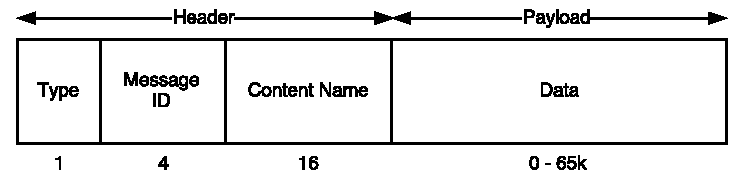
\includegraphics[width=1\textwidth]{images/packet.pdf}}
	\caption{\label{fig:packet} Application-layer message for content registration, advertisement, request and delivery. (adapted from: \cite{routeMultiGroup})}
\end{figure}

The message format can be seen in Figure \ref{fig:packet}, where "Type" refers to the purpose of the message, \textit{i.e.}, Content registration, Content advertisement, Content data, Content request, Relay election or notification of \gls{GO} role in another group and corresponding \glspl{ACK}. "Message identifier" is used to identify what message is an \gls{ACK} referring to. Content name is the MD5 hash of the content name. "Data" is the payload and can carry control or content data.\newline

K. Liu \textit{et. al} also provide a multi-hop routing implementation in \cite{manet}. The authors create a routing table composed by two sub-tables, one containing all peers that are directly discovered by the node and the other composed by peers that are accessible via other peers, \textit{i.e.}, multi-hop peers.

The first sub-table is created with a simple broadcast of the peer discovery signal and it will receive the responses from the devices in the vicinity, since in the authors' topology all devices are \glspl{GO} if no data is being transmitted. The response messages should contain the \gls{MAC} address of the destination devices, the gateway to reach the devices, in this case the node itself, since all nodes are neighbors and the number of hops to reach them, in this case zero.

After the first sub-table is complete all the nodes in the network have knowledge on who are their immediate peers. The nodes will then exchange routing table information between themselves to get a knowledge of all the multi-hop peers that may exist in the network. The second sub-table is filled proactively when nodes receive routing messages. The message-processing scheme is as follows: the device receives a message and checks its destination. If the destination \gls{MAC} is not the device's \gls{MAC} the device will look at its routing table and verify if an entry exists with that destination and where should the message be sent to, incrementing the number of hops, otherwise there is no route to the destination. If the destination \gls{MAC} is the device's \gls{MAC}, it will check the message type and infer if it is a routing message. If so, the device's routing table will be updated with the \gls{MAC} address of the source of the message, the \gls{MAC} address from where the node received the message, \textit{i.e.}, the gateway, and the number of hops necessary to reach the source.

\begin{figure}[ht]
	\noindent\makebox[\textwidth]
    {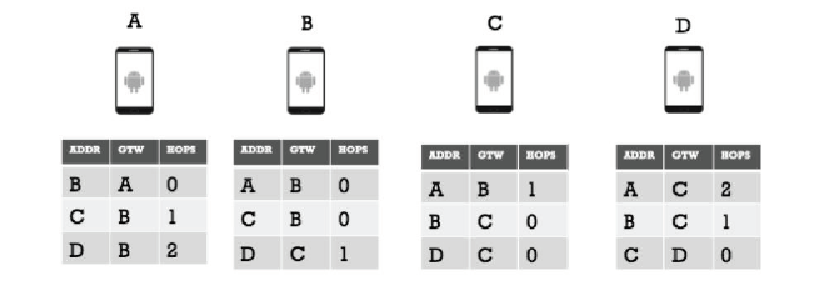
\includegraphics[width=1\textwidth]{images/routeTables.pdf}}
	\caption{\label{fig:routeTables} Wi-Fi P2P MANET routing table. (source: \cite{manet})}
\end{figure}

In Figure \ref{fig:routeTables} it is possible to see a complete table for four different nodes. Each node is now capable of sending a packet to its destination, without having to use a broadcast mechanism.

Two different routing mechanisms have been introduced in this section. Each mechanism is supported by a specific network scheme. This is the main problem of routing in Wi-Fi Direct, since the routing algorithm is developed at the application layer thus being always dependent on implementation, making most of the algorithms not compatible among themselves. This problem also brings some limitations in the number of users that will integrate a specific network with a specific routing scheme.













\section{Ad hoc Networking Applications in Android}
\label{sec:apps}

In this section some Android applications that make use of ad hoc networking will be presented, as well as the toolkits on which their development was based, if applicable. It is important in the scope of this work to know what are the offers on today's market on the ad hoc networking, to understand what has been done and what remains to be done and improved. These applications specifically make use of Wi-Fi Direct technology to establish communications or discover peers. It is worth mention that many other applications exist that create ad hoc networks but we are interested in the ones that use this technology in particular, since it will be the base to this work.

\subsection{FireChat}

FireChat is a cross-platform application that allows users to live chat with each other without access to the cellular or infrastructured network. It uses Bluetooth, Wi-Fi Direct or Apple Multipeer Connectivity to provide peer communication between devices.

FireChat is useful when there is a large concentration of users creating traffic that can, possibly, create some congestion in the infrastructured network. By using FireChat users are able to communicate between themselves with minimum delay, offloading the network and being independent on any service provider.

Users can create or join groups, \textit{a.k.a.} chat rooms, to communicate with other users in the same group. Messages can be sent to multiple or single destinations, also messages can be either private or public: in the first case only the selected receiver/receivers will be able to see the message. In the second case the message is broadcasted to all \glspl{GM} that form the chat room.

When a user sends a private message to another device, a private group is automatically created. However, senders might want to reach devices outside the groups where they are inserted, in that case the message is routed across the group as a private message to a \gls{GM} that is connected to the infrastructure and can send the message to the destination, that will receive it upon establishing Internet connection.

FireChat also allows for other features, such as blocking the communication with specific users, sending of photos, following other users' FireChat activity, \textit{etc.}.

This application is built with MeshKit, a \gls{SDK} module with methods allowing for P2P mesh connectivity within devices using this module. It is built over Bluetooth, \gls{BLE}, Wi-Fi Direct, ANT and other wireless protocols.

It works on three different mechanisms: cloud to mesh where devices connected to the Internet receive data from this link and share it with the other devices within its group, using one of the technologies mentioned above. The packets hop from device to device until it reaches the destination. This mechanism uses broadcast to diffuse the packets through the network.

The second mechanism is mesh to cloud where devices connected to the Internet forward data from devices without Internet connection but with a P2P connection established with the gateway devices, \textit{i.e.} the ones connected to the Internet.

Finally, the peer-to-peer mechanism, where the Internet is not accessed and devices transmit data between themselves using only the P2P link. Data is routed within the groups to reach its destination. Multicast or unicast transmissions can be used.

\subsection{Uepaa!}
\label{subsec:uepaa}

Uepaa! is one of the fastest growing P2P software companies, alongside with OpenGarden, responsible for FireChat. Uepaa! created Uepaa! Safety App, an application that aims to provide a security service for users who spend time outdoors and where cellular or Internet connection might not be available, such as mountaineers.

The app allows users to connect directly to the companies emergency call center even if no mobile network coverage is available in the area. This is achieved by forwarding the rescue message to users in the area using Uepaa!'s application. Similarly to FireChat's peer-to-cloud mechanism, in Ueppa! Safety App the message is routed through devices in the are until a device has a connection with either a mobile network or the Internet, and the rescue message, with the user's location is then sent to Uepaa!'s call center where the user can get assistance.

Uepaa! also developed the p2pkit a cross-platform \gls{SDK} that allows for P2P transmission of beacons, with configurable information. P2pKit also focuses on the battery consumption, since it can be used in battery sensitive applications such as Uepaa! Safety App. It provides P2P communication with all the associated processes, such as discovery and formation of groups. Range estimation on who are the closest peers and how close are they is also included in p2pkit modules, which can be useful to efficiently manage the battery of the device by sending only the beacons to the closest peers.

P2pkit is the base for different applications. Nearby devices using p2pkit are notified when a proximity event takes place and, although the principle is the same, applications are tailored to respond differently to certain types of events, \textit{e.g.} Uepaa! Safety App responds to the event of receiving a beacon by checking the device's Internet or mobile signal and tries to forward the message to the call center. other applications might trigger other responses, such as notifications to the current user, not forwarding the data but storing it and displaying it in the device.

\subsection{Murmur}

Murmur is an open-source, anonymous messaging application. Users can communicate with one another without Internet or mobile connection, similarly to the applications described above. However, Murmur uses Wi-Fi Direct and Bluetooth technologies to establish communications between the devices, creating a \gls{DTN} in which the P2P transmission of messages occurs.

Much like every other P2P network, the more users Murmur has, the faster transmission of data is. Messages are broadcasted over the network and if no device is in the vicinities of the sender, the message is queued for posterior transmission, thus the delay tolerant network designation. Murmur allows users to post messages to the network, a system to upvote, store, share and search for posts.

The discovery and connection between devices is done using both Wi-Fi Direct and Bluetooth: each user advertises it is running Murmur via the Wi-Fi Direct interface with a specific name, "MURMUR:Bluetooth MAC", constantly searching for peers using a similar device name, \textit{i.e.}, starting by "MURMUR". If a discovery is made, the application filters the Bluetooth \gls{MAC} address from the device's name and creates a Bluetooth connection, exchanging the message. The actual exchange starts with a handshake where each device sends its contact list and the amount of shared contacts between the two is calculated. Secondly, the number of expected messages to be exchanged is sent and, upon agreement, each device transmits until that number is reached. Finally, when the exchange is complete, the received messages are saved to a local database and the devices set a backoff time before establishing other connections, avoiding redundant exchanges and unnecessary battery consumption.












\chapter{Developed Peer-to-Peer Communication Prototype}
\label{chapter:work}

In this chapter the implementation of the developed peer-to-peer communication prototype will be analysed. This explanation will extend from the decisions of the technology and protocols to use to the architecture and workflow of the application.

It will begin with a brief summary of the steps taken to reach the developed application's features, functionalities and architecture. Which obstacles led to this solution and which were the fundamental drivers to decide upon this development and architecture to solve the problems previously stated. After the overall application's objectives and high-level architecture is described, a section on the lower-level architecture and components of the application will be presented, also containing flowcharts and diagrams on its normal functioning. A summary on the limitations and future work of this application will be given, as well as some possible solutions to its current limitations, outside the scope of this work. Finally, a conclusion on the difficulties and drawbacks of the development process and overall project appreciation will be given, along with some final thoughts on the work process and methods used.

\section{Peer-to-Peer Application Design Choices}

This section will provide the explanation and justification of the choices made for the application traffic type, ad hoc communication technology and ad hoc routing protocol.

In Section \ref{sec:wfd}, developed work on Android applications using Wi-Fi Direct has a mean of communication was introduced. Having the guidelines of these works in mind, the development of this application started. The main structure would always be: the application will have a routing algorithm that controls the destinations of the packets in each hop. A communication technology, \textit{e.g.} Bluetooth or Wi-Fi Direct, handler for both discovering nearby devices and establishing communication sockets with peers. A set of functions capable of analyzing incoming messages and deciding which is the next step to perform, in order to complete the requests/advertises. Finally, a user interface where the incoming messages can be seen and analysed (for debug purposes), also providing a text area for the user to enter the requested data.

\subsection{Application Traffic Type}

The choosing of what would be the transferred data between devices was one of the major steps of this work. Many ideas could be pursued and each one of them could be a great work to develop. The main contenders were text messages, beacon messages, geolocation messages and web pages. After some research was made, see Section \ref{sec:apps}, some of these contender could be eliminated, due to the existence of works already revolving around them. The main topic was text messages with many of the works developed focusing on recreating popular applications, such as Messenger and WhatsApp, using a peer-to-peer network to route the messages to their destinations. Beacon and geolocation messages were also not a completely innovative choice, since applications such as Uepaa!, see Subsection \ref{subsec:uepaa}, are already implementing systems similar to the one being proposed. Given this reasoning, the most innovative choice would be to transfer web pages between devices, creating a multi-hop hot spot in a peer-to-peer network.

\subsection{Ad Hoc Communication Technology}

After being established that web pages were the data to be requested, the next step was to choose the communication technology to be used, followed by the routing algorithm that would manage the next hops to take. The first and most obvious choice would be to use Wi-Fi Direct in both advertising and communication between devices, since this technology offers the best features to transfer files around 1Kbyte, in both range and data rate of transmission. However, during the development it proved to be impossible to continue with this approach, as Wi-Fi Direct's current Android implementation does not allow for devices to transfer files without user consent.

Given this drawback a shift to Bluetooth was made, and a hybrid version of the application was created, where the advertisement would be done via Wi-Fi Direct and the actual transfer of the web pages would be made via Bluetooth. This method also proved to be infeasible, due to security issues, since the the devices would have to display their Bluetooth MAC addresses in their Bluetooth name, making them much more vulnerable to possible attacks.

So, finally, the application was developed using Bluetooth for both advertisement of the devices and data transfer, although this is not the best technology for communication in a peer-to-peer network, it is the only one that, currently, meets all the requirements for this work. In the end of this chapter a brief discussion on the changes that need to be made to Wi-Fi Direct's implementation in Android will be presented, and why developers could benefit from these changes.

\subsection{Ad Hoc Routing Protocol}

The last step would be to create/modify a routing algorithm to control the destination of each incoming message. The requirements are simple, the algorithm simply needs to save the next hop of the shortest path leading to a device with Internet connection.

\gls{AODV} is a known routing scheme used in ad hoc mobile networks, precisely what this application will establish with the devices. However, it establishes dynamic paths, \textit{i.e.} only when a device wants to retrieve a web page does this protocol searches for a path in which to send the packet, see \cite{aodv} for the full specification of this scheme. This scheme is not the best for the applications reliability, since the requesting device should know before hand if it is capable of reaching the Internet, otherwise users will experience long periods of path requesting and advertising every time they request a web page.

\gls{DSDV} is also known for its use in ad hoc mobile networks. This protocol uses a routing table where it stores in each entry: the destination, next hop, number of hops to reach the destination and a sequence number - avoiding routing loops. The devices exchange full routing tables, creating a network where every device has total knowledge of the topology, being a powerful advantage. However, \gls{DSDV} requires the exchange of routing tables and their regular updates, using unnecessary bandwidth, see \cite{dsdv} for more information on \gls{DSDV}.

Since the routing of this work does not have a specific destination as a goal, in other words, device A does not want to transmit to B, it only wants to reach a node with network access with the minimum amount of hops, so A does not have knowledge on where its message will be sent after the immediate next hop. Thus, in order to accommodate such requirements some modifications were made to \gls{DSDV}. Firstly, to reduce the bandwidth used by \gls{DSDV}, this adaptation will simply exchange the best estimate of the current device, only including the number of hops and the device's \gls{MAC} address. Secondly, instead of a periodic exchange of tables, devices will update their tables every time a new advertise message is received and they only exchange routing information when a new best path is received, with the contents described above.

\section{Architecture}
\label{sec:architecture}

In this section the architectures of both framework and application are presented. It will consist of: a description of the Bluetooth connections between devices, an explanation on the discovery and advertising mechanism and a analysis of the web page exchange process.

\subsection{Bluetooth Connections}
\label{subsec:btconn}

In this subsection the Bluetooth connections between devices and their possible stages will be described and analysed.

Since the communication technology is Bluetooth, the application must have a thread\footnote{Thread is a sequence of instructions managed independently, usually by a scheduler from the operating system, see \cite{threads} for more documentation on threads.} that handles the listening and acceptance of connections and the data transfer between devices. This corresponds to the \textit{BluetoothService.java} class, from the application. It creates and listens to insecure communication sockets allowing devices to exchange data without user approval.

The service has three different threads within it: a thread for the acceptance of incoming communications - \textit{AcceptThread}, a thread for the initial exchange of vital information before the connection - \textit{ConnectThread} - and a thread for the actual exchange of data between devices - \textit{ConnectedThread}. The connection of devices goes through each of these stages, allowing the main thread to get information on what is the connection status of the device at a given time.

There were two different approaches to the connections of devices: either the devices stayed connected as long as possible until a new connection was requested or the devices stayed connected for the minimal amount of time for data to be transferred. The second approach was used, since it is the one that is more energy efficient, draining a lower amount of battery from the devices.

Bluetooth communication between devices is only allowed if both devices have matching "credentials", providing a minimum amount of security to prevent against possible attacks. An application specific name and \gls{UUID} represent the application, making it distinguishable from any other, since the \gls{UUID} of an application should not be repeated in any other.

To notify the application of what is being done by the \textit{BluetoothService} a handler is created, acting as bridge between the two parts. It can be used for various actions, such as: retrieving the status of a connection, assessing if a device is ready to receive a file, \textit{etc.}

To substantiate the possible Bluetooth connections stages four different textual representations are created, one for each stage: listening, connecting, connected and not enabled. Each type of thread mentioned earlier is associated with one stage, being the non-existence of a thread the not enabled stage. The different threads can be seen as the implementation of a stage. They are the ones that dictate how is the application going to act during the stage. 

In the next subsections each stage will be explained in detail, providing a better understanding on how the connections are performed.

\subsubsection{Listening}
\label{subsubsec:listening}

A device is said to be in the listening stage when it has no ongoing connection but it is waiting for a new one initiated by another device. It is the "first" stage of the \textit{BluetoothService}, since every time the service is initiated the device is moved to this stage.

As was said previously, each connection stage is associated with a thread class. The listening stage is associated with the \textit{AcceptThread}, which is instantiated every time the device enters this stage. The framework's connections have short durations and each time a new connection is performed the service is restarted, entering the listening stage. Hence, it is imperative to assure there are no memory leaks or communication sockets left open. Thus, before the listening thread is instantiated it is verified if any other Bluetooth connection threads are running and, if so, they are shut down.

Once all the requirements for the instantiation of a new thread are met, a communication socket is created with which the device listens to incoming communications. To implement the listening mechanism a loop is created whose purpose is to block the thread until a new connection is received, an error occurs or the user shuts down the application.

Whenever the device receives a new connection, it verifies the "credentials" sent in that request and compares them with the ones defined in its \textit{BluetoothService}. If they match the connection is accepted.

Upon successfully accepting a connection, the method assesses the status of the newly formed connection and decides upon it. If everything goes as planned, the connection should now be in the connected stage. Once this migration between stages is concluded the instance of the listening thread is destroyed, for reasons above stated and the 

\begin{figure}[ht]
	\noindent\makebox[\textwidth]
	{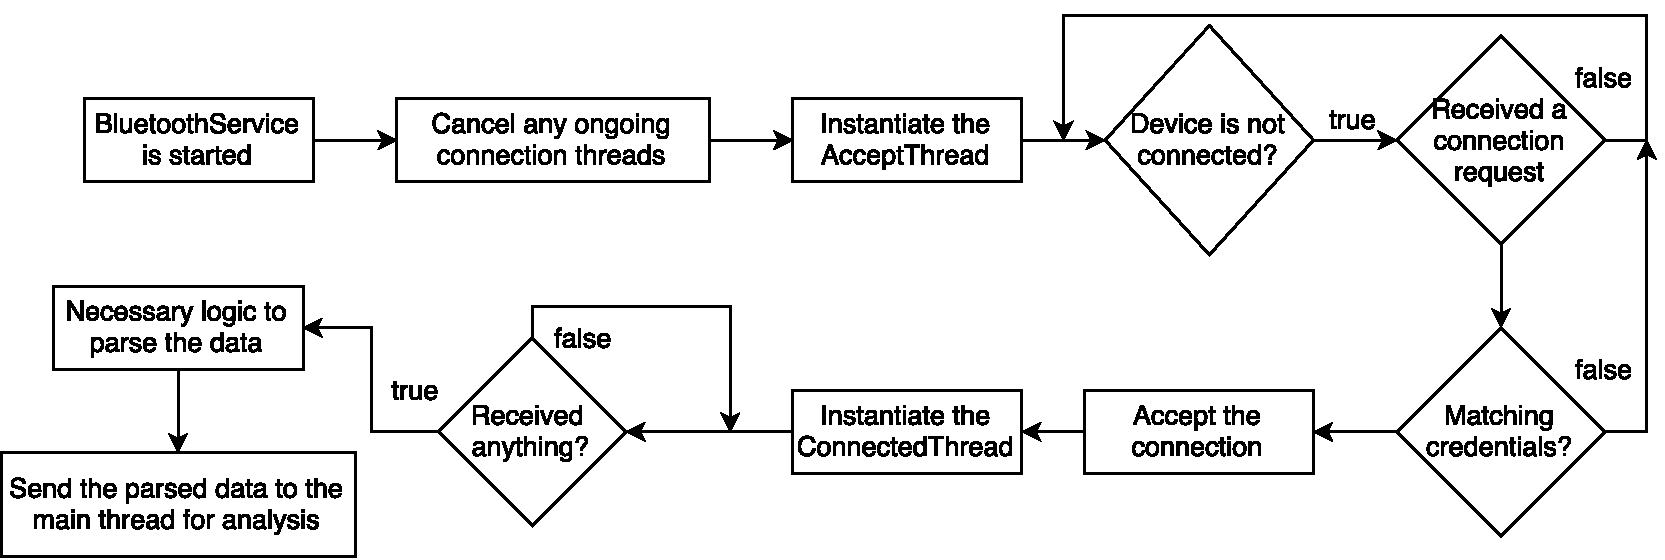
\includegraphics[width=1\textwidth]{images/btreceiver.pdf}}
	\caption{\label{fig:btreceiver} Fluxogram of a Bluetooth connection receiver's performed actions}
\end{figure}

In Figure \ref{fig:btreceiver} it is possible to see the performed actions from the point of view of a device that is waiting for incoming connections. It starts when the \textit{BluetoothService} is initiated and finishes when the received bytes are sent to the application for analysis, described in \ref{subsubsec:connected}.

\subsubsection{Connecting}
\label{subsubsec:connecting}

Concluded the listening and accepting of connections it is necessary to understand how they are requested. For a Bluetooth connection to be performed at least two devices must exist, one of them acting as the connection requester.

Similar to the listening thread initiation, the \textit{ConnectThread} is only instantiated after all the previous Bluetooth connection threads running in the device are shut down. Also, to avoid delays during the connection process, the Bluetooth discovery process is shut down. Only then can the requester attempt to establish a connection with the desired device.

To identify the receiver of the connection request, the device needs to retrieve the \gls{MAC} address of its counterpart, this will be explained in Subsection \ref{subsec:disandadv}. Once this is attained the requester can attempt to create a communication socket between both devices, using the previously defined Bluetooth "credentials" and the receiver's \gls{MAC} address. If the \gls{MAC} address is valid and corresponds to a device within reach the connection is request successfully.

In case of failure due to the rejection of the connection from the receiver, a notification is sent to the application, notifying the connection was not successful and the service is restarted.

However, if the sent request is accepted by the receiver, the connection state is assessed and, if no interruptions or errors occur, the connection stage is moved to the connected stage, indicating both devices are able to send and receive bytes from their counterpart, by writing and reading from the established communication socket, respectively.

\begin{figure}[ht]
	\noindent\makebox[\textwidth]
	{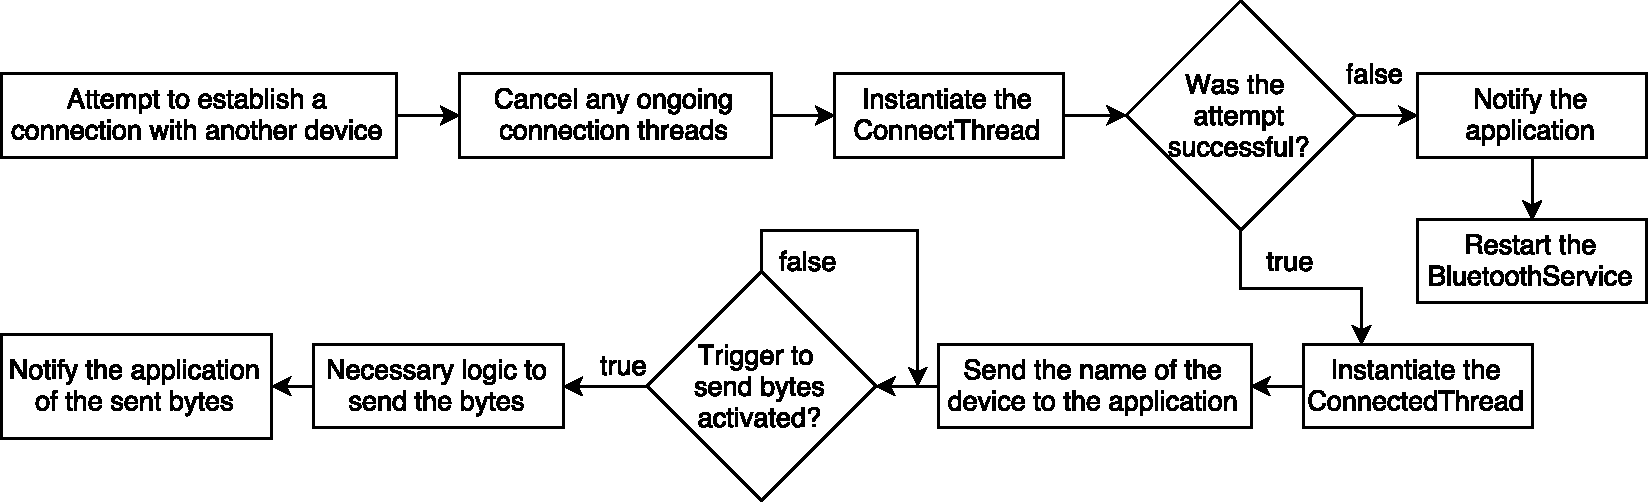
\includegraphics[width=1\textwidth]{images/btrequester.pdf}}
	\caption{\label{fig:btrequester} Fluxogram of a Bluetooth connection requester's performed actions}
\end{figure}

In Figure \ref{fig:btrequester} the actions performed by a Bluetooth connection requester can be seen. Beginning by the attempt to establish a connection to the notification of the successfully sent bytes, described in the next subsection.

\subsubsection{Connected}
\label{subsubsec:connected}

When the connection reaches the connected state both requester and receiver devices are linked through a Bluetooth communication socket. To start the receiving and transmitting mechanisms a \textit{ConnectedThread} is created, after all ongoing threads are cancelled to avoid conflicts between communications or memory leaks. To notify the application of the connection success the service sends the counterpart's Bluetooth identifier, \textit{i.e.} its Bluetooth name, to the application.

To understand how data is transferred between the two connected devices it is necessary to explain two different mechanisms: the writing of data and the reading of data. By creating a socket linking both devices two data streams are also created, implicitly, where one provides a stream to write data into the socket and the other provides a stream to read data from the socket, see Figure \ref{fig:inoutstreams}. Both writing and reading data is in the form of byte arrays that can be posteriorly manipulated into the desired format.

\begin{figure}[ht]
	\noindent\makebox[\textwidth]
	{
\includegraphics[width=0.8\textwidth]{images/inoutstreams.pdf}}
	\caption{\label{fig:inoutstreams} Communication channel with input and output streams}
\end{figure}

The writing of bytes into the socket is done through an output stream, name given to the part of the stream that handles the writing. For any data format the principle is the same, to convert the data into a byte array that will be sent through the stream. It is important to note that the channel has a limited size buffer shrinking the arrays' size, thus if the data to be exchanged has a large amount of bytes, it is wise to create a cycle that sends parts of that data, instead of the whole. The writing process is asynchronous, since it is only executed at a certain time following a certain trigger, \textit{e.g.} user input. It is possible to notify the application of the sent bytes if they are relevant to other processes, \textit{e.g.} notifying that a text message was sent and prepare to receive/send an image.

The reading of data from the socket is done through an input stream. Since the output stream only writes byte arrays into the socket the input stream will only read byte arrays. This property burdens the developer with the task of treating the received bytes, \textit{i.e.} converting them to their original data type. Also, as mentioned before, the communication socket has a limited size buffer, thus it is also the developer's responsibility to create the reception cycle, following the premises used to create the sending cycle, \textit{e.g.} read the same amount of bytes sent. This mechanism may need to comprise the necessary logic to aggregate the multiple byte arrays received, if the original data was divided and sent in several parts. The reception loop is running while the connection remains active and whenever bytes are read from the socket, these are sent to the application to be analysed and converted back to their original format.

To send and receive different data formats within the same application it is needed to develop a protocol to handle the different conversions of the sent and received byte arrays. Further along this chapter it will be explained how this was done in the developed application to exchange both text messages and web pages.

\subsection{Discovery and Advertising}
\label{subsec:disandadv}

Now that the basic concepts on how the communication between devices are implemented are explained, it is possible to dig deeper into the intrinsics of the application itself, and what is the logic behind the routing of web pages.

The first thing in order for each device to know what is the next hop of a certain request will be to fill the routing tables. This process is done by a series of discoveries\footnote{Discovery is the act of finding nearby devices with Bluetooth on.} and advertisements\footnote{Advertise is the act of notifying peer devices of the cost of relaying a request to the device issuing the advertisement.}. Upon starting the main activity, each device will advertise its best estimate to reach the Internet. This advertisement will be received by peers and analysed. In case the estimate of relaying the requests through that node improves the current estimate, the receiving peer will begin another discovery and advertising process with the newly discovered path. Otherwise, the peer will add or update an entry in the routing table, regarding the advertiser.

\begin{figure}[ht]
   \noindent\makebox[\textwidth]
    {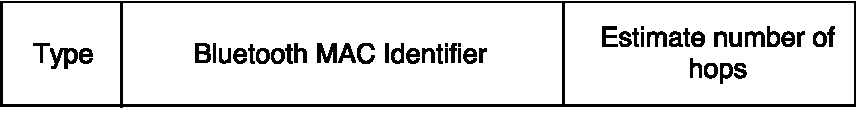
\includegraphics[width=0.7\textwidth]{images/adv_message.pdf}}
	\caption{\label{fig:advmsg} Advertising message format}
\end{figure}

In Figure \ref{fig:advmsg} the format of an advertise message is shown. The type is a feature common to all messages exchanged in this application. It servers the purpose of identifying which type of message is being received. It can take four different values: \textit{ADV}, \textit{RQT}, \textit{RSP} and \textit{FAIL} for an advertisement, request, response and fail message, respectively. In this case it will take the value \textit{ADV}. The delimiters of the different message parts - vertical lines in Figure \ref{fig:advmsg} - are represented by the dot comma character (;), in order to be able to separate the different parts of the message. The Bluetooth \gls{MAC} identifier is always the \gls{MAC} address of the Bluetooth adapter of the sender, it is then used by the receiver to populate its routing table. Finally, the estimate number of hops is the smallest number of hops the sender needs to be able to reach the Internet plus one, corresponding to the hop from the receiver to the sender.

Each device has two different routing tables: one that is used to store the information retrieved from the advertisement process, providing the best path for routing the requests to the final device. Other that is used to route the responses back to the original sender, as explained in the next subsection. For simplicity the first routing table will be referred by the same name, while the second will be referred to as response table, as it handles the routing of responses.

\begin{table}[ht]
\centering
\bgroup
\def\arraystretch{2.5}
\begin{tabular}{|c|c|}
\hline
\textbf{Next hop's MAC} & \textbf{Number of hops} \\ \hline
Own MAC & 0 or 16 \\ \hline
Device A's MAC & Estimate through A \\ \hline
Device B's MAC & Estimate through B \\ \hline
... & ... \\ \hline
Device Z's MAC & Estimate through Z \\ \hline
\end{tabular}
\egroup
\caption{Routing table example and format}
\label{tab:routTables}
\end{table}

In Table \ref{tab:routTables}, an example of a routing table is presented, where the first entry is always populated with the device's own \gls{MAC} address and its estimate, which is either 0 or 16\footnote{16 was chosen to be the representation of infinity or inability to reach a destination, since it has been represented by this number in various protocols, for instance in \gls{RIP}, see \cite{ripprotocol}}, meaning the device has an Internet connection or not, respectively. Every time a device receives an advertisement message, it populates this table, either by adding a new row or updating an existing one, with the information contained in the message - see Figure \ref{fig:advmsg}. When the routing table is done being populated, each node knows its immediate peers and the best estimate through each one of those peers, giving it a full knowledge of its vicinity, \textit{i.e.}, the sub-network created by the peers that are reached by the device using a single hop.

In the code, this process was implemented, mainly, in \textit{RoutingApp.java} class and in the main activity, or \textit{BtActivity.java}. Let's start by understanding how the routing tables are being created and, posteriorly, it will be explained how and when they are populated. It is important to note that \textit{RoutingApp} class extends the Java class \textit{Application}, meaning that, with the exception of the private methods and variables, every part of this code can be accessed at any time in the application, in contrast with other activities that are only accessible when active, such as \textit{BtActivity} and \textit{InitActivity}.

In appendix \ref{appendix:RoutingApp} it is possible to see the definition of two tables \textit{routeTable} and \textit{rspTable}, corresponding to the routing table and response table, respectively. In this subsection's scope a closer look will be taken on the first table. It is represented as an instance of the Java interface Map\footnote{In Java, a Map is an object that relates keys to values. To a single key corresponds a single value, thus not creating duplicate entries, see \cite{map} for full documentation.} where the keys correspond to the \gls{MAC} address of the next hop, the string, and the keys to the respective estimated number of hops, the integer. So it maps a string to an integer, which is the same to say that given a string the table contains, it will return an integer.

There are three important features that the application needs from this table: to get the absolute minimum value, meaning retrieving the lowest possible value for any given key, in order to retrieve the device's best path. To get the corresponding key to the minimum value, in order to retrieve the receiver to whom this device should send the message. Finally, to update or add a row with a new key-value pair, in order to add newly received advertising information.

The first feature is completed by method \textit{getMinHop()}. This function starts by creating a variable \textit{minHop}, that will be assigned to the minimum value of the table. It then makes use of the preexisting Java method \textit{Collections.min()}, that returns the minimum value from a set of values, and assigns the variable \textit{minHop} to this value. To get the desired value, it is given the set of values of the routing table, by calling \textit{routeTable.values()}. Should this succeed, the function will return the desired value, otherwise it will return 16, for the reasons explained above.

Having the minimum value from the routing table, it is now necessary to retrieve the \gls{MAC} address from the device that provides this estimate. This is done by function \textit{getKeyFromValue()}, that receives the routing table itself and the desired value. It iterates through every key and, in every iteration, it compares the value of the current key to the expected value, since it already knows the minimum value it is useless to compare the values of the different keys. If, in a given iteration, it finds a key that maps to the desired value, this key will be returning, corresponding to \gls{MAC} address of a device that gives the smaller estimated number of hops, otherwise it returns null. It is important to note that several devices may provide the shortest path, but the application will only chose the one that was found first, since they all provide the same estimate.

Finally, the addition and update of rows within the table is done by the method \textit{updateRouteTable()}, that takes as arguments the newly received advertising message. It begins by fragmenting the message in its parts, knowing that, according to Figure \ref{fig:advmsg}, this message will contain the type in the first position\footnote{In Java, the first position of an array is given by the number 0, the second by the number 1 and so forth, see \cite{arrays} for more information.}, the sender's \gls{MAC} address in the second position and the estimated number of hops in the third, using dot commas as delimiters. Using Java method \textit{String.split()}, the function separates the string by dot commas, creating an array of smaller strings, it then matches the destination to the second position, represented by variable \textit{dest}, and the number of hops to the third position, represented by variable \textit{hops}. Having this information, the Java method \textit{Map.put()} is used, it inserts the given key-value pair into the existing table, in case this key already maps to a value, the value will be overwritten with the new one, otherwise it will simply insert the new pair as a new row, see \cite{map} for full documentation on this method. 

Note that, in case of a table update, the application does not compare values, \textit{i.e.}, it does not check if the new estimate is better than the old one, since the sender device could have lost the communication with the best route and thus it needs to advertise a worse path. If this check was made, the receiver could be mislead into sending requests through this device, thinking it would provide the better path.

\subsubsection{Discovering Peers}
\label{subsubsec:disc}

Now that it is clear how the intern process of modifying the routing tables works, it is possible to discuss where and when these methods are being called. Shifting the focus to \textit{BtActivity.java}, in appendix \ref{appendix:BtActivity}, there are some variable definitions indispensable for the process of advertising and discovery. Starting by the \textit{peers} \textit{ArrayList}, it is a list of \textit{BluetoothDevices} each corresponding to a peer found in the discovery process. This list is then used to retrieve information from these devices, in order to successfully establish communication sockets with them. The \textit{mBluetoothAdapter} is no more than the device's Bluetooth adapter, without which there would be no Bluetooth communications. Finally, the variable \textit{discoveryFinished} is a boolean value that serves the purpose of identifying if the discovery process is finished, assuring that this is not carried away for longer than it was intended to be, using processing power and damaging the performance of the rest of the application.

Method \textit{onStart()} is used to denote the starting of the activity. It  starts by verifying the necessary steps to ensure Bluetooth is properly set. Some configurations relative to an \textit{WebView} object, that will be discussed later, are performed. The \textit{ensureDiscoverable()} method is called, in which the application checks the Bluetooth visibility of this and, in case it is not discoverable, it sets the visibility to 0, that corresponds to "always visible", see \cite{btandroid}.

Once the Bluetooth is set up, the initial update of the routing table is performed, a quick network check indicates if the device has an active Internet connection, by calling the method \textit{getHasNet()}, from \textit{RoutingApp.java} class, in appendix \ref{appendix:RoutingApp}. Should the device return positive, it will add a new row with its own \gls{MAC} address, retrieved by method \textit{getOwnMAC()} and 0 hops, since it's connection is immediate. In case the Internet check returns negative, meaning the device is currently unable to reach it, the same process is performed, however instead of 0 hops, the estimate will be of 16 hops, for reasons already explained.

The device is now finished with the first steps of assessing its position in the network and filling its routing table accordingly. After this logic is accomplished the function \textit{doDiscovery()} is called, it sets the variable \textit{discoveryFinished} to false, indicating the discovery is not yet finished and commands the Bluetooth adapter of the device to initiate the discovery process.

Figure \ref{fig:adveg1} demonstrates how two devices, one without an Internet connection (left) and one with an active Internet connection (right). At this point both devices should have exactly one entry at their routing tables, since they have not communicated with any other device but they have established their position in the network, \textit{i.e.}, if they have an Internet connection. Device A is unable to reach the Internet, so it adds to the routing table an entry with its own \gls{MAC} address and an estimate of 16 hops. Device B, on the other hand, is able to reach the Internet, thus having an entry with its own \gls{MAC} address and an estimate of 0 hops.

\begin{figure}[ht]
   \noindent\makebox[\textwidth]
    {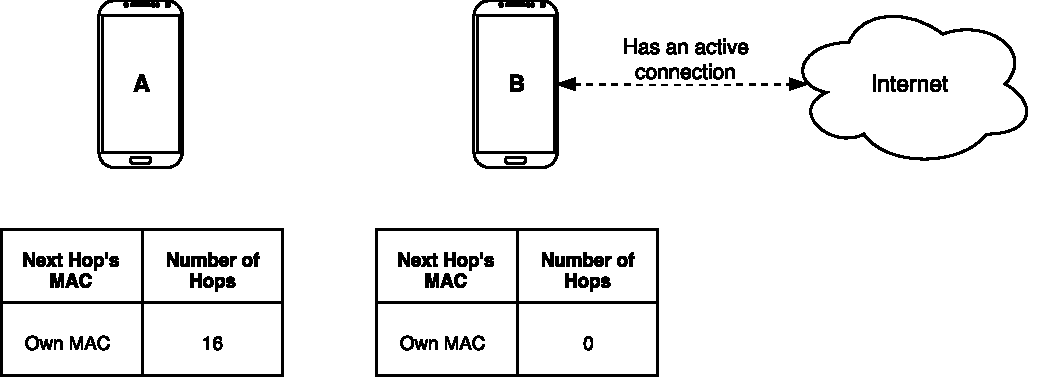
\includegraphics[width=0.9\textwidth]{images/adv_example_1.pdf}}
	\caption{\label{fig:adveg1} Example 1: State of the two devices after the initial step is over}
\end{figure}

Jumping now to the definition of the \textit{BroadcastReceiver mReceiver}, responsible for the management of the Bluetooth discovery process and peers found, we can see that it is divided into two main sections: one for the management of a peer found and other for the management of the finished discovery. In the first segment, whenever a device is found, a new \textit{BluetoothDevice} object is created, to designate the found peer, this peers is the added to the list \textit{peers}, unless this device is already part of this list. In the second segment, corresponding to the finish of the discovery process, the receiver checks if the variable \textit{discoveryFinished} has been toggled on, meaning it's the first time the device has received an \textit{ACTION\_DISCOVERY\_FINISHED} action, which is self-explanatory, so the discovery should be canceled, by \textit{cancelDiscovery()} and the variable \textit{discoveryFinished} needs to be set to true.

In Figure \ref{fig:discflux} a fluxogram of the discovery process is presented. By following the Figure it is possible to understand the flow of the code and the hierarchy of instructions. It is a visual representation of the code running. Note that it ends with the instruction \textit{advertisePeers()} that will be explained shortly.

\begin{figure}[ht]
   \noindent\makebox[\textwidth]
    {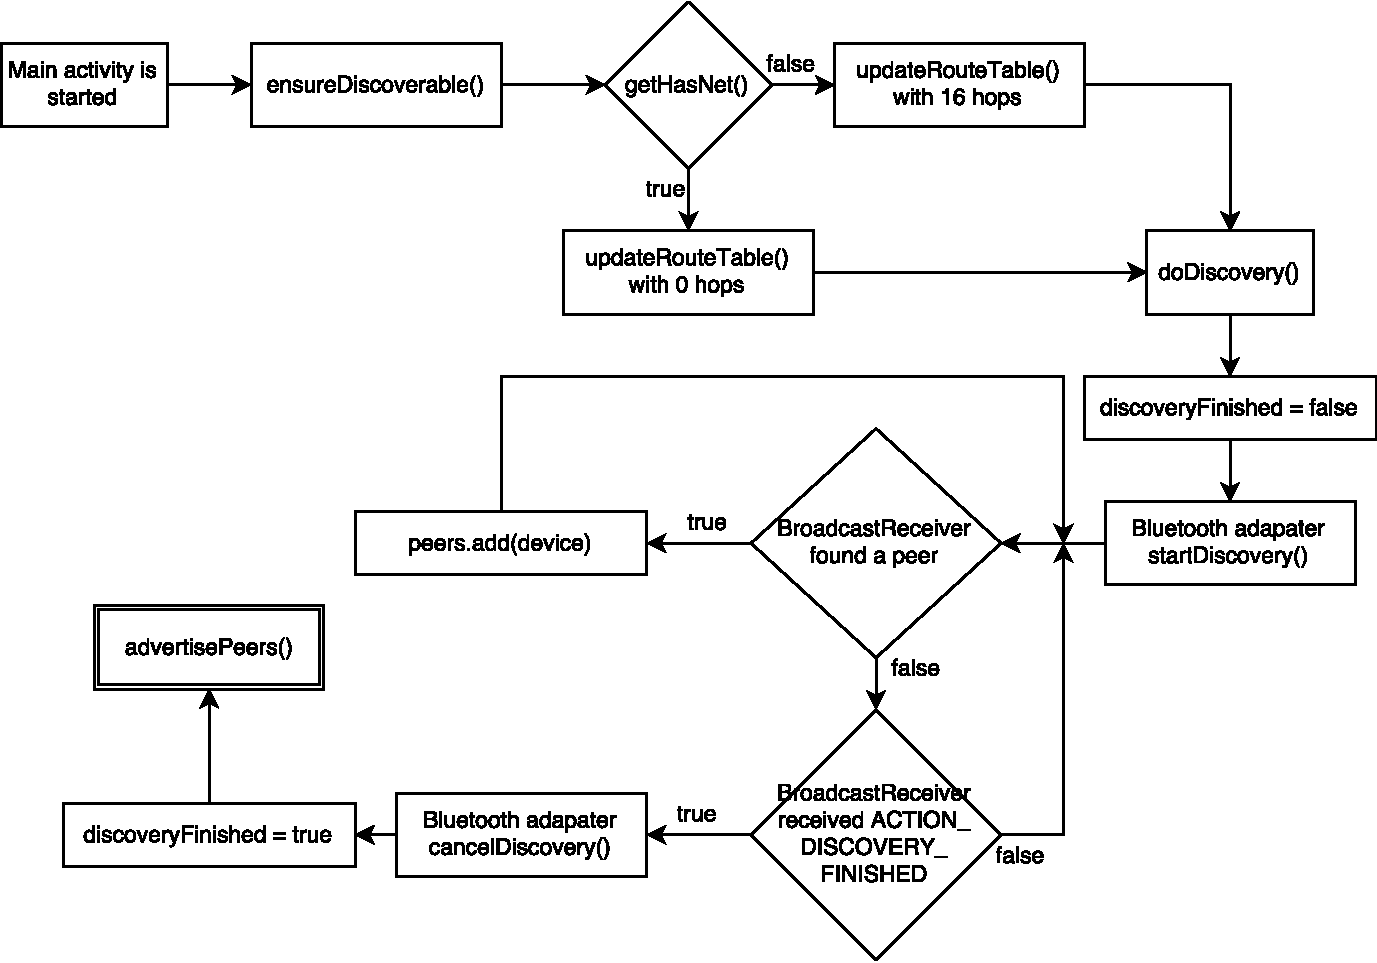
\includegraphics[width=1\textwidth]{images/discovery_flux.pdf}}
	\caption{\label{fig:discflux} Fluxogram of the discovery process}
\end{figure}

\subsubsection{Sending an Advertising Message}
\label{subsubsec:sendadv}

The device has now found its peers and it can start the advertising process, done by \textit{advertisePeers()}. The method starts by iterating through each peer contained in the list \textit{peers}, a first check is performed assessing if the device is a smart phone or a different type of device, a sensor or a headset, for instance, for this the \textit{DeviceClass} is compared with 524, which is the value for smart phones, see \cite{btclass}. 
In case the peer is a smart phone, a quick check to the name is performed, in order to see if it contains a dot comma at the beginning of the name. This is simply a test measure and can be deactivated, it is only to reduce the number of connections to the ones where the other device is, effectively, using the application.

After the necessary checks are processed, if the peer device is eligible for connection, the \textit{BluetoothService} method \textit{connect} is called, see \ref{subsubsec:connecting}. To ensure the message is not sent before the connection is established, a small loop was created. This loop will be seen throughout the application, since it proved to be an efficient way to ensure the connection was established before the message was sent. It "blocks" the method until the Bluetooth state is \textit{STATE\_CONNECTED}, see \ref{subsubsec:connected}, inside the cycle there is a verification if the state does not change to \textit{STATE\_LISTEN}, as this would mean the device is not attempting to establish a connection anymore and it is simply listening for incoming requests. In case this is verified, the \textit{BluetoothService} is restarted and the application assumes the connection has failed.

If the method breaks the cycle normally, meaning the connection was established successfully, the function \textit{getMinHop()} is called returning the value of the minimum estimate of the device and 1 is added, symbolizing the hop this message will take from sender to receiver. The message is then sent, with the format seen in Figure \ref{fig:advmsg}, where the device's \gls{MAC} is retrieved by method \textit{getOwnMAC()}.

Finally, the method enters another cycle, this time for ensuring this device does not try to advertise to a new peer whilst it is sending a message to the previous one. For that, the \textit{initTime} variable is set to the current time and the method is "blocked" while the Bluetooth status is not \textit{STATE\_LISTEN}, see \ref{subsubsec:listening}. In case the method is "blocked" for more than 5 seconds, the application assumes something went wrong proceeding to break the cycle and continues the program normally. Usually, the cycle should be over way before the 5 seconds mark. Once the cycle is over or broken, the method iterates to the next peer and proceeds to do the same tasks.

In Figure \ref{fig:advflux} the fluxogram of the advertising process is presented. It shows how the \textit{advertisePeers()} method works in a simple way. In the end of this method's execution the application's \textit{BluetoothService} keeps listening for incoming connections of its surroundings.

\begin{figure}[ht]
   \noindent\makebox[\textwidth]
    {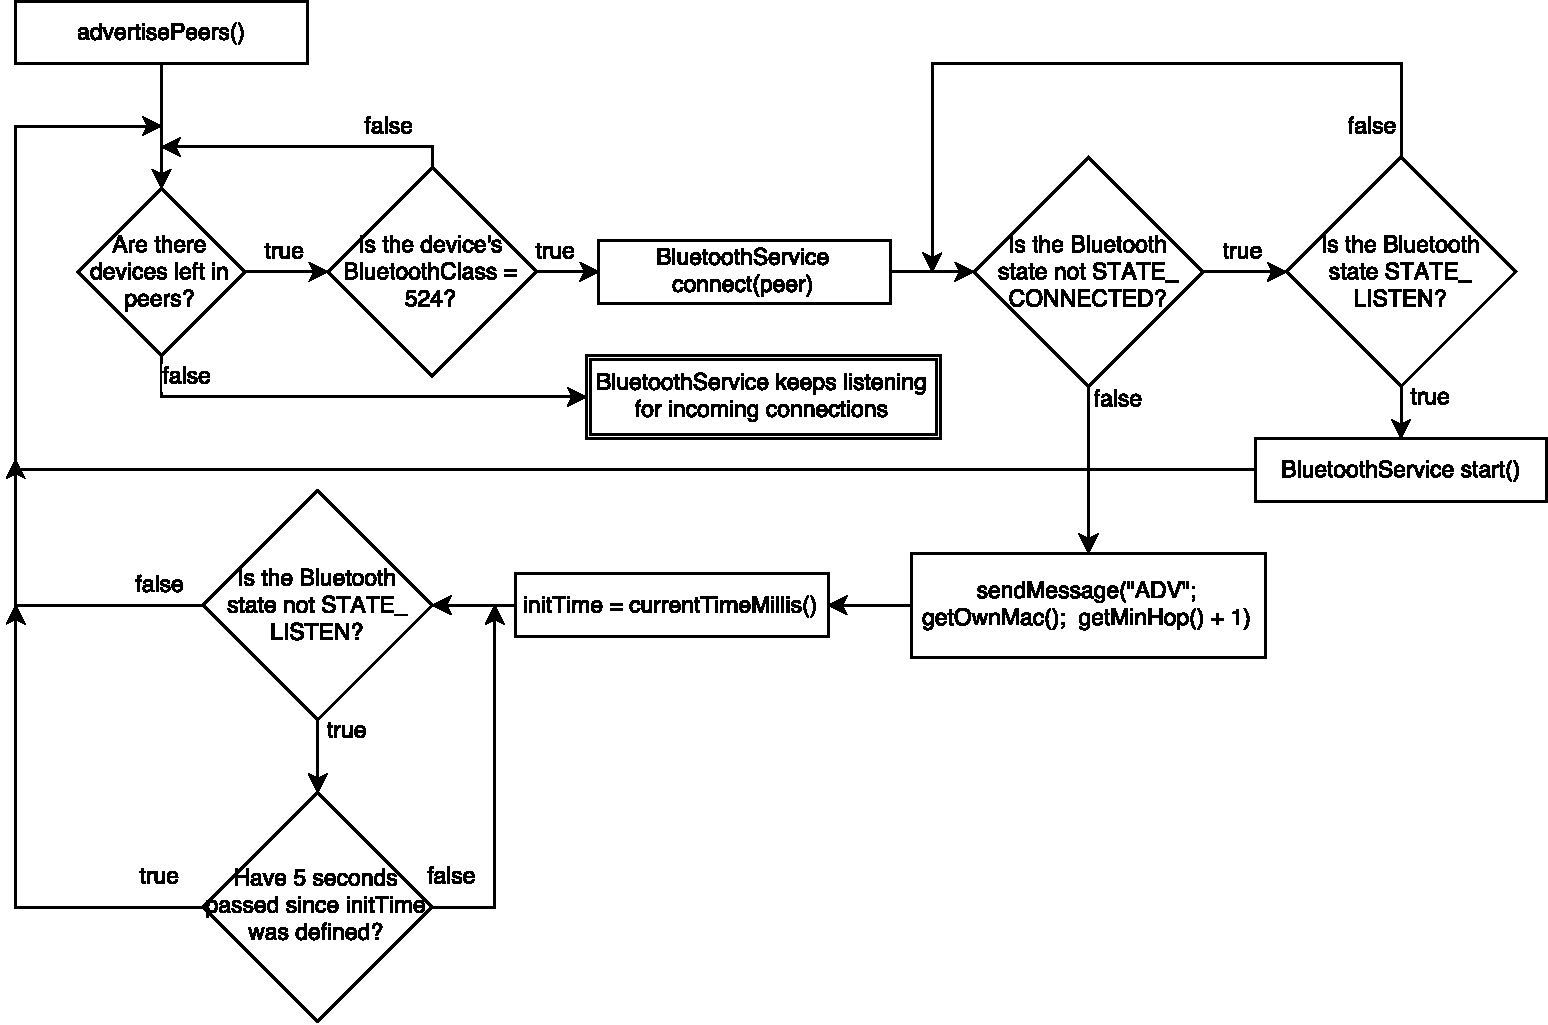
\includegraphics[width=1\textwidth]{images/advertise_flux.pdf}}
	\caption{\label{fig:advflux} Fluxogram of the advertising process from the point of a sender}
\end{figure}

\subsubsection{Receiving an Advertising Message}
\label{subsubsec:rcvadv}

It is now covered how the transmitter of an advertise message operates, however, to fully understand the advertising process it is necessary to analyse the receiver device and how it handles this message.

So, on the receiver device, after the reception of the advertising message, the handler receives the transferred message bytes from the \textit{BluetoothService}. To understand how this is performed the \textit{Handler mHandler} must be explained first.

The method \textit{handleMessage()} is overwritten, in order to control what is done with the received \textit{Message}, see \cite{msgclass} for full documentation on this Android class. There are seven possible \textit{Message} types: \textit{MESSAGE\_STATE\_CHANGE} used to notify of a Bluetooth state change, \textit{MESSAGE\_WRITE} received when this device has sent a message, \textit{MESSAGE\_READ} to notify that this device has just received a message, \textit{MESSAGE\_DEVICE\_NAME} received when there is a new connection, gives the name of the connected device, \textit{MESSAGE\_TOAST} for when the user needs to be notified on something regarding the \textit{BluetoothService}, \textit{FILE\_READ} to notify of the reception of a web page by the device and \textit{FILE\_WRITE} for debug purposes, received when this device sends a web page.

For the receiver's advertising process the focus will be on the \textit{MESSAGE\_READ} \textit{Message} type. If the \textit{Message} is identified as a \textit{MESSAGE\_READ} the \textit{Handler} will construct a \textit{String} from the received bytes. From this \textit{String}, the device is now able to extract what type of message it is, \textit{i.e.}, an \textit{ADV}, a \textit{RQT}, a \textit{RSP} or a \textit{FAIL}. In case the message is not a response the \textit{BluetoothService} is restarted and will listen to incoming connections. However, if the message is a response, the service is not restarted, this will be analysed in the next subsection.

After the message is converted to a \textit{String}, it is passed to the method \textit{analyzeMessage()}, where the device will see how to deal with the received message. Here, the message type is assessed, in this case the focus will be the \textit{ADV} type. If the message is identified as an advertising message the method will extract its estimate and compare it to the device's best estimate, retrieved from \textit{getMinHop()}. If the comparison concludes the received estimate does not top the previous best, the routing table is updated with the received estimate and \gls{MAC} address, through \textit{updateRouteTable()}, previously explained. Otherwise, it means the device has found a better way to reach the Internet, so after the routing table is updated, the variable \textit{discoveryFinished} is set to false and the discovery process is done again, through the method \textit{doDiscovery()}.

\begin{figure}[ht]
   \noindent\makebox[\textwidth]
    {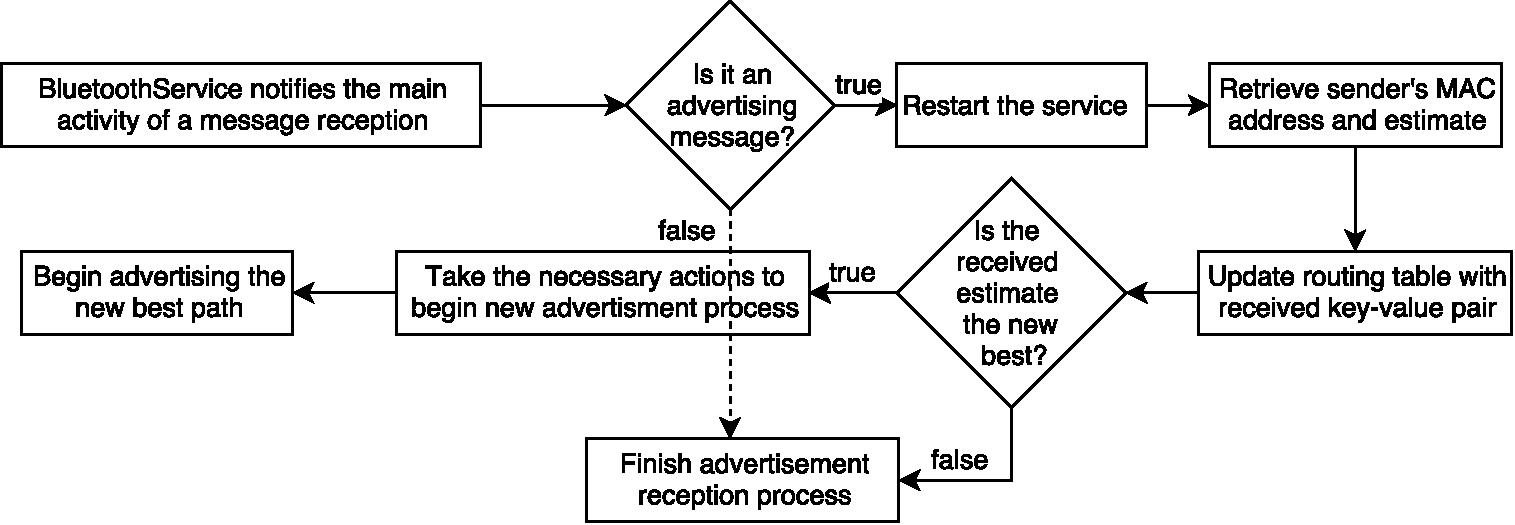
\includegraphics[width=1\textwidth]{images/recv_advertise_flux.pdf}}
	\caption{\label{fig:recvadvflux} Fluxogram of the advertising process from the point of a receiver}
\end{figure}

In Figure \ref{fig:recvadvflux} it is shown a fluxogram for a receiver device and its order of instructions. The device ends this process either with a \textit{doDiscovery()} method call or by "listening" to incoming connections. Some aspects of the fluxogram are simplified as they do not concern this process and will be discussed later.

\begin{figure}[ht]
   \noindent\makebox[\textwidth]
    {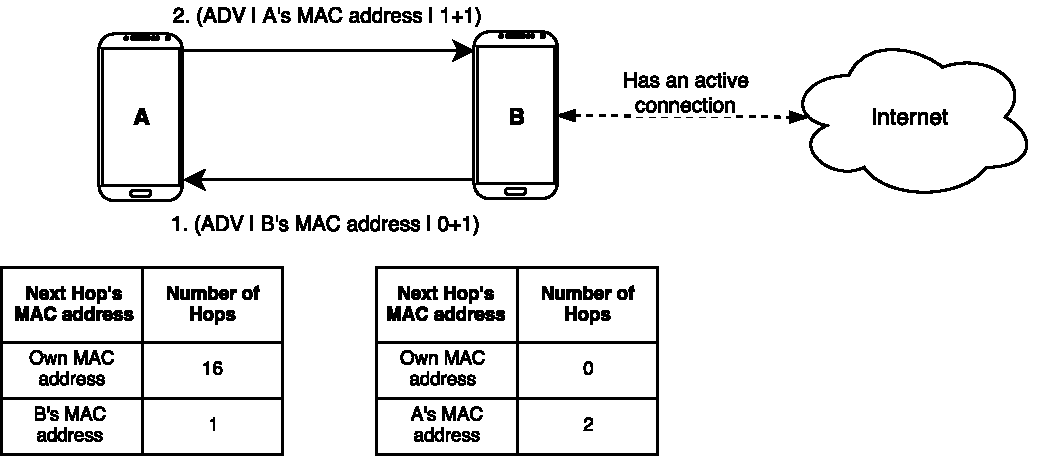
\includegraphics[width=1\textwidth]{images/adv_example_2.pdf}}
	\caption{\label{fig:adveg2} Example 1: State of the two devices after the advertising process is done} 
\end{figure}

To summarize, in Figure \ref{fig:adveg2} the example with devices A and B from Figure \ref{fig:adveg1} is extended. Now device B has advertised to its peers, which include device A. Upon receiving this message, device A proceeded to store the information in its routing table, followed by and advertise from itself, since the new estimate tops the previous one. After this is concluded both devices have the shown routing tables, and A knows it routes to B, while B routes to itself, since A provides a poorer estimate.

If A advertises first the result would be the same, since when B is advertising A would still receive a better estimate and would advertise again. When B receives the second advertise from A it will overwrite the previous entry, maintaining the same values.

Now it should be clear how the discovery and advertising process is performed and what is the code executed at each time of the process. This is the basis of the next subsection, since without it the devices would not be able to reach the Internet unless they already had the connection.

By giving each device a full view of its vicinity it is possible to establish a network in which every device knows the best path instantly. This is done by what was described above, from discovery to advertisement. The next subsection will refer to the next step, where the devices already have their routing tables populated and are ready to exchange web pages. 

\subsection{Exchange of Web Pages}

In this subsection the logic created and implemented to exchange the web pages will be explained, in detail, also an example, similar to the previous one will be shown to better demonstrate the processes. This analysis will be mainly focused in appendix \ref{appendix:BtActivity}. However, before that it is necessary to explain the routing table related to the exchange of web pages, previously mentioned in Subsection \ref{subsec:disandadv} and referred to as response table.

The main purpose of this table is to provide a destination for a response message. Once a device has received a request and it has an Internet connection, it should know where to send back the response. This would be easy if only this case applied, it would simply send back the response from where it received the request. But, in the case this device is a "bridge" node, \textit{i.e.}, it is simply a node that forwarded a request, it may have received requests from different devices and it still needs to be able to differentiate each message and decide which device to send back the response to.

The response table has a similar structure to the routing table, see Table \ref{tab:rspTables}, but it serves a different purpose. Similarly to routing table, the response table is defined in \textit{RoutingApp} class, it is an object of the Java class \textit{Map}.

\begin{table}[ht]
\centering
\bgroup
\def\arraystretch{2.5}
\begin{tabular}{|c|c|}
\hline
\textbf{Message ID} & \textbf{Next hop's MAC} \\ \hline
Message ID \#1 & Device X's MAC \\ \hline
Message ID \#2 & Device Y's MAC \\ \hline
Message ID \#3 & Device Z's MAC \\ \hline
... & ... \\ \hline
Message ID \#9 & Device X's MAC \\ \hline
\end{tabular}
\egroup
\caption{Response table example and format}
\label{tab:rspTables}
\end{table}

Despite the similarities, there is one difference between the two: routing table maps \textit{Strings} to integers whereas response table maps integers to \textit{Strings}. The latter is used to associate message identifiers, the integers, with the \gls{MAC} address of the next destination of a response, the \textit{String}.

The table is defined as \textit{rspTable} and it has two associated methods: \textit{updateRspTable()} and \textit{getRspHop()}. The first method is used to add new rows to the response table, it is similar to routing table's method \textit{updateRouteTable()}, and makes use of the same Java method \textit{put()}, previously explained. Although it has a slight difference in logic, since this method will not update rows, it will always insert new rows, seeing the message identifiers are unique there should be no duplicate entries.

The second method, \textit{getRspHop()} is used to retrieve the \gls{MAC} address associated to a certain message identifier, that is as a parameter. In case a table entry is found for that specific identifier, the associated \gls{MAC} address is returned, otherwise it will return null, notifying the application that no entry was found and thus, the response will not be routed.

For the example three devices are used: A, B and C. Where device C has an active Internet connection, as seen in Figure \ref{fig:example1.0}. In this figure it is possible to see the routing tables of each device after this process is completed. Device A will choose B to send a request and B will choose C, since they provide the best estimates, respectively.

\begin{figure}[ht]
   \noindent\makebox[\textwidth]
    {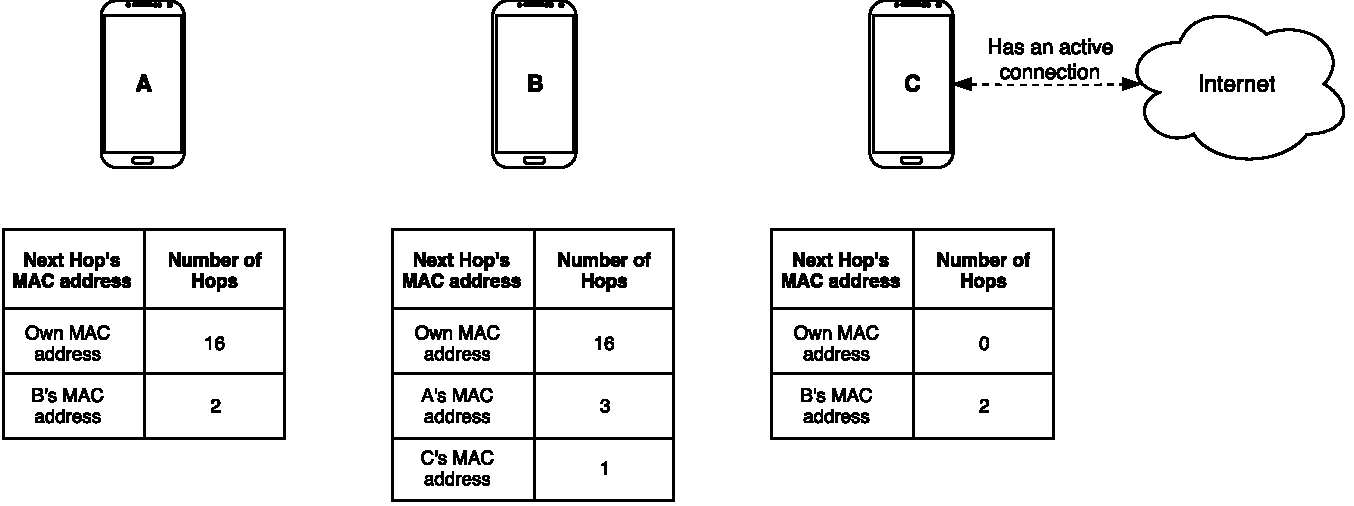
\includegraphics[width=1\textwidth]{images/example_1_0.pdf}}
	\caption{\label{fig:example1.0} Example 2: State of the routing tables of the three devices}
\end{figure}

\subsubsection{Sending a Request Message}
\label{subsubsec:sendrqt}

Now that the logic and implementation behind the response table is understood it is possible to start explaining the actual process of web page exchanging. Starting by the definition of variables, in \textit{BtActivity} class, it can be divided into three sections: the first being the definition of variables that will identify the different elements seen by the user, a \textit{Button}, to submit requests, an \textit{EditText}, for the user to input the requested \gls{URL} and a \textit{WebView}, to manage the actions related to web pages.

It is then possible to see the definition of the constants relative to the \textit{BluetoothService} class, see \ref{subsec:btconn}. The possible \textit{Message} types received from the service are defined: \textit{MESSAGE\_STATE\_CHANGE}, \textit{MESSAGE\_READ}, \textit{MESSAGE\_WRITE}, \textit{MESSAGE\_DEVICE\_NAME}, \textit{MESSAGE\_TOAST}, \textit{FILE\_READ} and \textit{FILE\_WRITE}. These types are explained in \ref{subsubsec:rcvadv}, and \textit{MESSAGE\_READ} was already mentioned, although only covering the advertising messages.

Finally, the last block of variables, containing various definitions relative to this class. \textit{msgID} is the variable that concerns this process of exchange, it stores the message identifier of the last received request or response.

\begin{figure}[ht]
   \noindent\makebox[\textwidth]
    {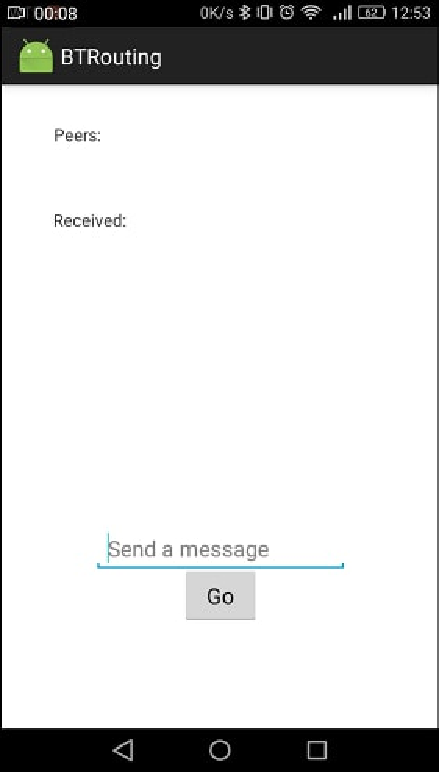
\includegraphics[width=0.3\textwidth]{images/initScreen.pdf}}
	\caption{\label{fig:initScreen} User interface for the sending of request messages}
\end{figure}

In Figure \ref{fig:initScreen} it can be seen the display of the main activity page, it has five main elements: a place where the \textit{peers} list will be displayed, at the top. The received messages, this is optional and used for debugging as it would incur in severe security issues, so it should be removed if not for debugging. An \textit{EditText}, see \cite{edittext} for documentation on this Android feature, used to allow the user to input the web page he/she desires and to capture this input to be processed. A \textit{Button}, to notify the activity it should now begin the process of requesting the web page. Finally, a \textit{WebView}, see \cite{webview} for documentation on this feature, that is hidden from user view and will remain so until the user receives the response to its request.

Assuming the device already established the best route to reach the Internet, the journey of the request, from the user input to the display of the response, will be explained. Starting by the user input, has said above, a \textit{Button} and an \textit{EditView} are defined, so a user interface is created, in order to send requests based on the user input. This is defined in method \textit{onStart()}, from appendix \ref{appendix:BtActivity}, after the routing table is first populated and the discovery is started, discussed in \ref{subsec:disandadv}. The variables previously defined, \textit{goButton} and \textit{mEdit} are matched to the elements in Figure \ref{fig:initScreen}, so they can be identified by the application.

The \textit{Button} class' method \textit{onClick()} is then overwritten, meaning it is tailored for the specific needs of this application. This method has the purpose of responding to a click of the user in the specific button, to this click the method must associate an intent to send a request message. With these parameters the method \textit{onClick()} is set to call \textit{sendRequest()}.

The \textit{sendRequest()} method receives as parameters: a boolean to identify if the intent is coming from the owner of the request or from a mediator node, an integer that corresponds to the message identifier and a \textit{String} containing the requested \gls{URL}.

Since this particular request comes directly from the user input, this method is initially called by this device with the following arguments: "true", "-1" and the user input text. The "true" value is used whenever the device is the one issuing the request, \textit{i.e.}, whenever it is its origin. "-1" is used when the value of the message identifier is not important, in this case, since this device is the "owner" of the request, a random message identifier will be generated. Finally, to identify the web page requested, the user input \gls{URL} is passed.

\begin{figure}[ht]
   \noindent\makebox[\textwidth]
    {
\includegraphics[width=0.9\textwidth]{images/rqtmessage.pdf}}
	\caption{\label{fig:rqtmsg} Request message format}
\end{figure}

In Figure \ref{fig:rqtmsg} a generic request message is shown. Its format does not differ much from the one presented in Figure \ref{fig:advmsg}, however there is a new field, the \textit{Message ID}, a unique identifier representing each message that will be useful to keep track of what is each message's payload and sender. The \textit{\gls{URL} to request} is the web page's \gls{URL} the user is trying to access, it is considered to be the payload of the message.

Continuing the analysis on method \textit{sendRequest()}, the first thing that is done is to retrieve the next hop, to whom the device shall send its request, this is done by calling the method \textit{getNextHop()}, defined in \ref{appendix:RoutingApp}. This method returns the \gls{MAC} address of the device's peer who provides the best path. \textit{getMinHop()} is called to retrieve the best estimate, to which is applied the function \textit{getKeyFromValue()}, alongside with the routing table, see Subsection \ref{subsubsec:disc} to get more a detailed explanation on how these two methods work. This combination should return the desired \gls{MAC} address, however if the best estimate is 16, "null" is returned to notify the device that no path was found.

Once the \gls{MAC} address of the next hop is attained, \textit{sendRequest()} compares it with "null", to ensure there is an actual device to connect to. In case this comparison is successful, meaning there is no next hop, the method \textit{sendFail()} is called. Since this device is the owner of the request, the \textit{sendFail()} method will not send a failure notification to another device, it will simply notify the user of the failure. The method \textit{sendFail()} will be discussed further on this subsection.

In the case of the device having a valid next hop, the connection is performed, similarly to the advertising connections, by the \textit{BluetoothService connect()} method. The first cycle described in the advertising process is now repeated here, to ensure the connection is established before sending the message, with the single difference of in case of failure, \textit{i.e.}, the Bluetooth state becoming \textit{STATE\_LISTEN}, \textit{sendFail()} is called again, to notify possible predecessors of this request, however in this case it does not apply.

If the cycle is finished and everything is completed without any incidents, the method verifies the first argument, the boolean variable to identify if the device is the owner of the request. If the device is the owner a random message identifier is generated through the Java class \textit{Random}, see \cite{random}. Once the identifier is generated, the message is sent with the parameters: "RQT" as \textit{Type}, the value of the generated random as \textit{Message ID}, the device's \gls{MAC} address gotten through \textit{getOwnMAC()} as \textit{Bluetooth MAC Identifier} and the received \gls{URL} from the arguments as the \textit{\gls{URL} to request}, as seen in Figure \ref{fig:rqtmsg}. The response table is also updated with the newly generated message identifier and device's \gls{MAC} address, through \textit{updateRspTable()}.

Otherwise, if the device is not deemed as the owner, there is no random identifier generation, since the value will come from the received request. Also the response table is not updated, since it will be updated earlier in the receiving process, that will be the next focus. However, the message is sent as before, with the slight difference that the \textit{Message ID} is now the one received as an argument.

\begin{figure}[ht]
   \noindent\makebox[\textwidth]
    {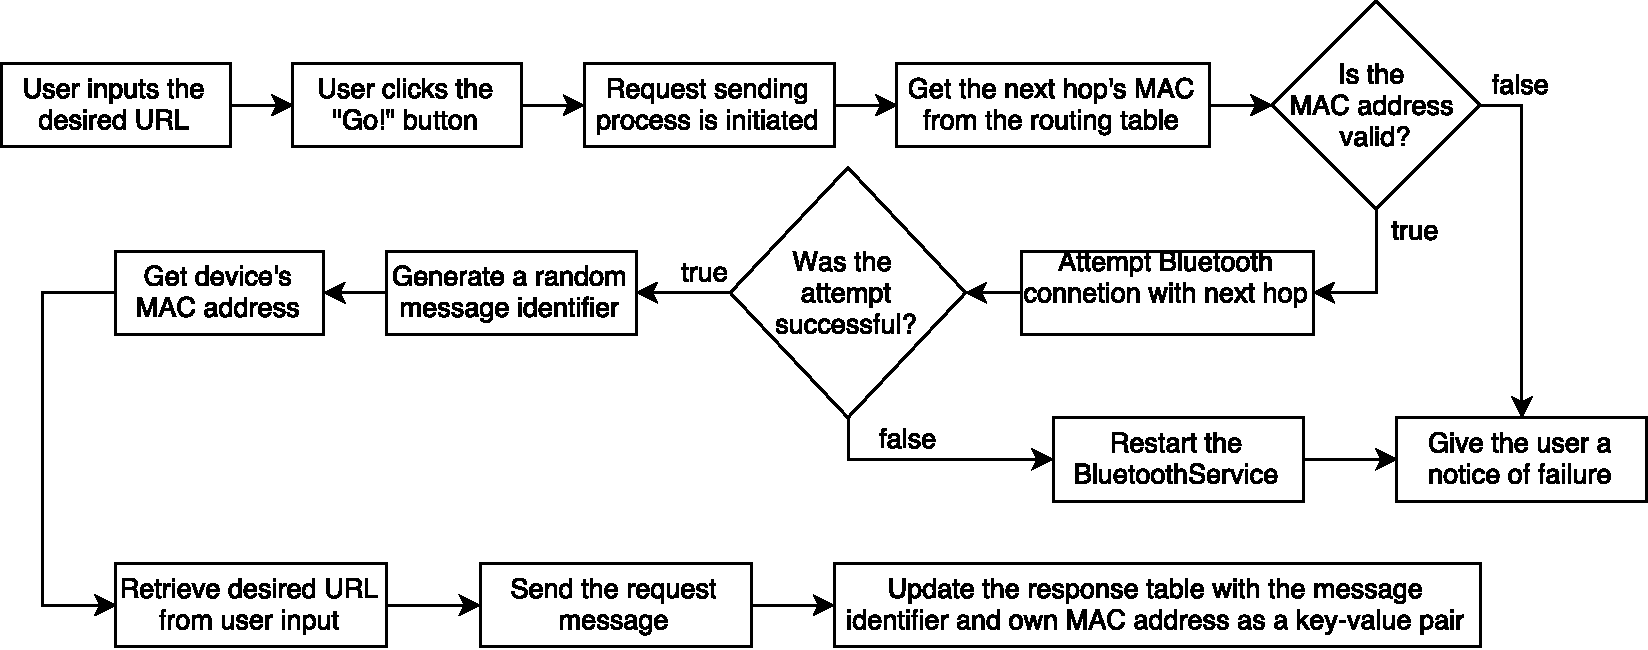
\includegraphics[width=1\textwidth]{images/rqtflux.pdf}}
	\caption{\label{fig:rqtflux} Fluxogram of the request sending process}
\end{figure}

In figure \ref{fig:rqtflux} a fluxogram representing the process of sending request message is presented. It provides a better overview of the code hierarchy, and when is each method called. Once the process is finished the device keeps listening to incoming connections, changing the Bluetooth state to \textit{STATE\_LISTEN}.

\subsubsection{Receiving a Request Message}
\label{subsubsec:rcvrqt}

The request receiving process is similar to the advertise, the receiver connects to the sender and receives the bytes from the request sent. As before, the bytes are transmitted from the \textit{BluetoothService} to the main activity, through a \textit{MESSAGE\_READ Message} and the \textit{mHandler} receives them. After comparing the received \textit{Message} to the possible types, explained in Subsection \ref{subsubsec:rcvadv}, and concluding it is a \textit{MESSAGE\_READ} the \textit{Handler} converts them to a \textit{String}. Since the newly created \textit{String} is not a response, the \textit{BluetoothService} is restarted and \textit{analyzeMessage()} is called taking as argument the \textit{String}.

In \textit{analyzeMessage()} the argument \textit{String} is compared to the possible message types, \textit{ADV}, \textit{RQT}, \textit{RSP} and \textit{FAIL}. It will now be identified as a response, due to the analysis of the message type, see Figure \ref{fig:rqtmsg}, and immediately the message identifier is saved in the variable \textit{msgID}.

In the request sending process it was mentioned that, in case the device was not the owner of request, it would not update the response table. This was due to the fact that, for the devices that are not the owners of the request, this process is done here, in \textit{analyzeMessage()}. So, the routing table is updated with the message identifier and \gls{MAC} address of the sender, retrieved from the message.

Two different approaches can now be taken: one regards the devices with Internet connection and the other the devices without one. To define which approach is taken by the device a quick check of the Internet connection status is performed, via the method \textit{getHasNet()}. If the result is false, meaning the device has no Internet connection, the request will be forwarded to the next hop to reach a device with Internet. To do this, the device calls \textit{sendRequest()} with arguments: false, the message identifier, retrieved from the received message and the \gls{URL} requested, also retrieved from the message. The method follows the same steps as before, described in \ref{subsubsec:sendrqt}.

If the result of the \textit{getHasNet()} query returns true, it means the device has an Internet connection and, as such, it is a final destination. This means the device will now be the communication link with the Internet and it needs to retrieve the requested web page and send it backwards until it reaches the owner of the request. This process begins by calling the method \textit{getPage()}, that receives the requested \gls{URL} and the message identifier, both retrieved from the received message.

In \textit{getPage()} the web page is downloaded via the \textit{WebView}, mentioned in \ref{subsubsec:sendrqt}. A new \textit{WebViewClient} is created, see \cite{webview} for documentation on \textit{WebView} and its features, such as the \textit{WebViewClient}. This client is different from the usual, since the device does not want to display the downloaded page.

The methodology to save the web page had several possibilities, such as saving the web page as an image, saving only the \textit{HTML} content or saving each element of the page individually. The first two methods are not complete, meaning the web page could lose some of its features, \textit{e.g.} dynamic images, search fields, \textit{etc.}. The third method would fully download the web page, however it would require additional logic to save the different elements in the same directory and to arrange them to re-create the web page with its initial format.

The method \textit{saveWebArchive()} provides a complete solution to this problem, it is a method specific to the \textit{WebViewClient}'s class, see \cite{webview} and it solves the problem of third method, since it downloads each element but compiles them in a web archive, that can be decompressed easily by \textit{WebView}. Thus, it proved to be the better solution for this problem.

To implement this methodology, the method \textit{onPageFinished()}, from \textit{WebViewClient}'s class, is overwritten. This method is used to do something after the web page is finished loading. So, a new \textit{File} is created in the application's directory, with the name "file.mht". If the file creation succeeds, the web page is downloaded and saved in the created file, via \textit{saveWebArchive()}. In order to guarantee the web page is downloaded and saved before the response is set, a \textit{waitForWebPage} downloader is created and executed.

The \textit{waitForWebPage} class can be seen in appendix \ref{appendix:BtActivity} and was created with the sole purpose of guaranteeing the web page transfer is completed before the response is sent. If this check is not performed, it is possible that, for large web pages, the response file will be incomplete and thus not displaying correctly the requested \gls{URL}.

It extends an \textit{AsyncTask}, used to perform background operations and send the results to the main thread, see \cite{async} for the full documentation. It starts by creating a variable \textit{file} that will contain the address where the web page will be saved. The method \textit{doInBackground()} is overwritten, as it always has to be in an \textit{AsyncTask}, since it contains what operations to be performed.

In this method it is continuously checked if the variable \textit{file} has a size bigger than 0 bytes. Whenever this condition is verified, it means the web page was saved successfully. The \textit{onPostExecute()} method, used to send the results to the main thread, is also overwritten and, once this thread reaches this point, it means the device is ready to send the response, so \textit{sendResponse()} is called.

\begin{figure}[ht]
   \noindent\makebox[\textwidth]
    {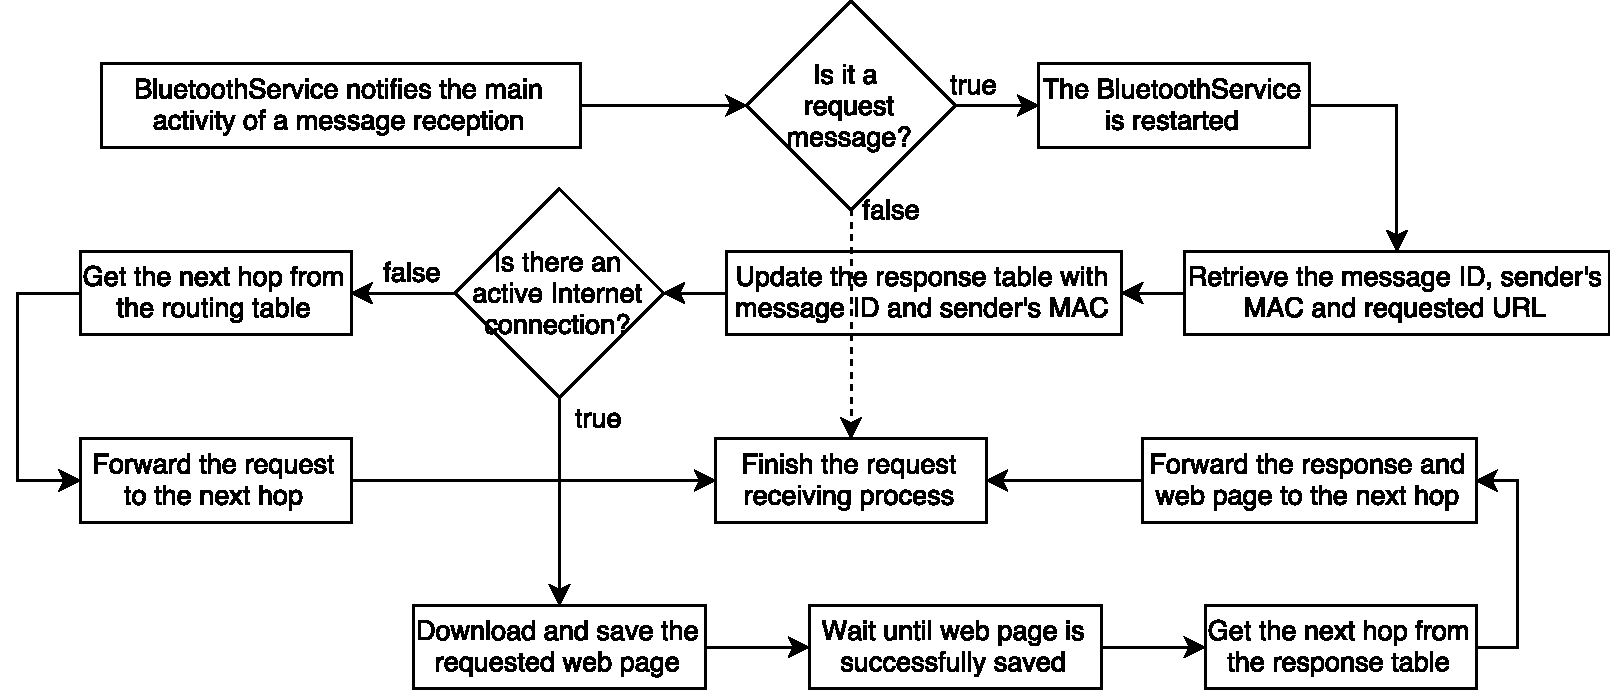
\includegraphics[width=1\textwidth]{images/rqt_rcv_flux.pdf}}
	\caption{\label{fig:rqtrcvflux} Fluxogram of the request receiving process}
\end{figure}

In Figure \ref{fig:rqtrcvflux} it is possible to see a fluxogram of this process. The process, as shown in the figure, ends either with sending a new response or a new request, depending on whether the device has Internet connection or not, respectively.

\begin{figure}[ht]
   \noindent\makebox[\textwidth]
    {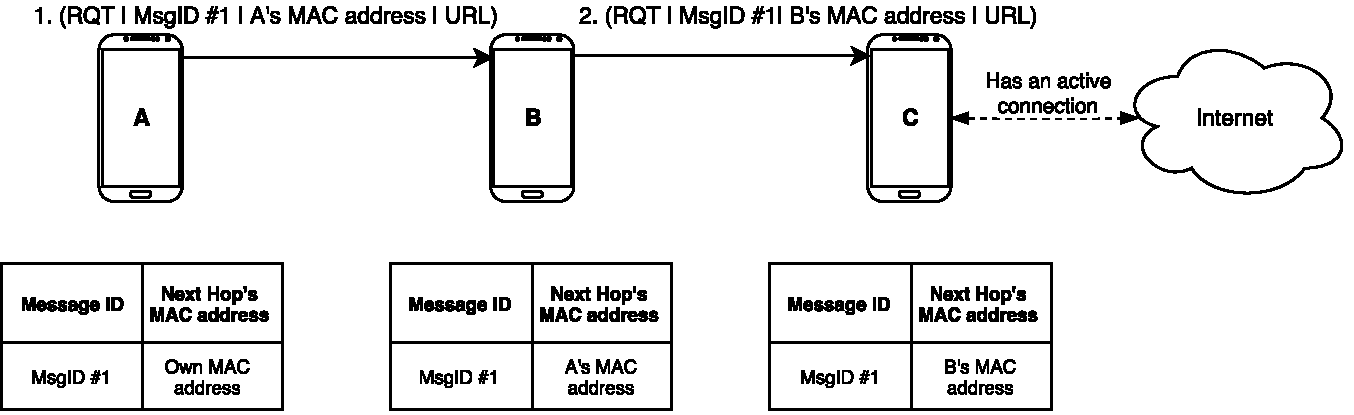
\includegraphics[width=1\textwidth]{images/example_1_1.pdf}}
	\caption{\label{fig:example1.1} Example 2: Request sending and receiving process}
\end{figure}

Resuming the example in Figure \ref{fig:example1.0} and supposing the user from device A wants to request a \gls{URL} and inputs it correctly, the device will follow the steps explained in Subsection \ref{subsubsec:sendrqt} and check the routing table to establish the next hop. Also its response table will be filled during this action, since it is the owner of the request.

Once that process is completed and the message reaches device B it will update its routing table with the newly received request. After that it checks its own routing table and assesses if it should forward the request or download the page. Since the device does not have an active connection the first option will chosen and the request forwarded to C.

Finally, upon receiving the request, device C will update its own response table with the received message identifier and B's \gls{MAC} address. Having an Internet connection the device will download the web page.

In Figure \ref{fig:example1.1} it is shown the above described, as well as the three response tables from the devices once the requests are all sent and the web page downloaded.

\subsubsection{Sending a Response Message and Web Page}
\label{subsubsec:sendrsp}

Once the web page is successfully saved in the device it is possible to send the response back until the owner of the request receives the requested web page. As seen before, \textit{sendResponse()} is called in \textit{onPostExecute()} and it is used to send a response to the next device.

It receives as parameter the message identifier, so that the \gls{MAC} address of the next device can be retrieved from the response table. Thus, having the message identifier and through the method \textit{getRspHop()}, the device retrieves the next hop's \gls{MAC} address. Should the result of this call be null, the response will not be sent. If the result returns a valid \gls{MAC} address, the connection process is performed, along with the cycle to ensure the connection is successful, described in Subsection \ref{subsubsec:sendadv}.

\begin{figure}[ht]
   \noindent\makebox[\textwidth]
    {
\includegraphics[width=0.4\textwidth]{images/rspmessage.pdf}}
	\caption{\label{fig:rspmsg} Format of a response message}
\end{figure}

Finally, if all the above goes as planned and succeeds, the response is sent with the format seen in Figure \ref{fig:rspmsg}, with "RSP" as \textit{Type} and the received argument \textit{msgID} as \textit{Message ID}.

The next step is to send the actual web page to the next hop, but first the sender needs to ensure the response was correctly sent. This is done by the \textit{Handler}, explained in Subsection \ref{subsubsec:sendadv}. The \textit{Message} type \textit{MESSAGE\_WRITE} is used for this, since it returns the bytes sent from the device and convert them to a \textit{String}. If the converted \textit{String} is a response message the application concludes the process is completed correctly and proceeds to call the method \textit{sendFile()}.

The \textit{sendFile()} method is called when the device is ready to sent the web page bytes to the next hop. It begins by creating a variable \textit{file}, pointing to the file in the application storage that contains the web page. The size of that file is retrieved through \textit{file.length()} and an array of bytes is created with that same size. This array of bytes will be the place where the web page will be transferred, from the internal storage to the application.

In order to transfer the web page from the file, in the internal storage, to the application a \textit{BufferedInputStream} is used, see \cite{bis} for more documentation on this class. This \textit{BufferedInputStream} instance takes the bytes from the variable \textit{file}, previously described and saves them in the array of bytes, it is then closed to avoid memory leaks.

Once the bytes are transferred to the application the device needs to send them to the next hop, since the connection is still opened, for reasons that will be explained in the next subsection, it is possible to send the bytes without the logic to connect to the next hop. The method \textit{writeFile()} from \textit{BluetoothService} is called and the file bytes is transferred to the next hop as described in Subsection \ref{subsubsec:connected}.

The method gets the number of bytes to be sent and divides that size by 990 bytes, getting the number of chunks that need to be sent to the next hop. It then proceeds to send each chunk with a length of 990 bytes, until it reaches the last chunk, sending the remaining bytes.

\begin{figure}[ht]
   \noindent\makebox[\textwidth]
    {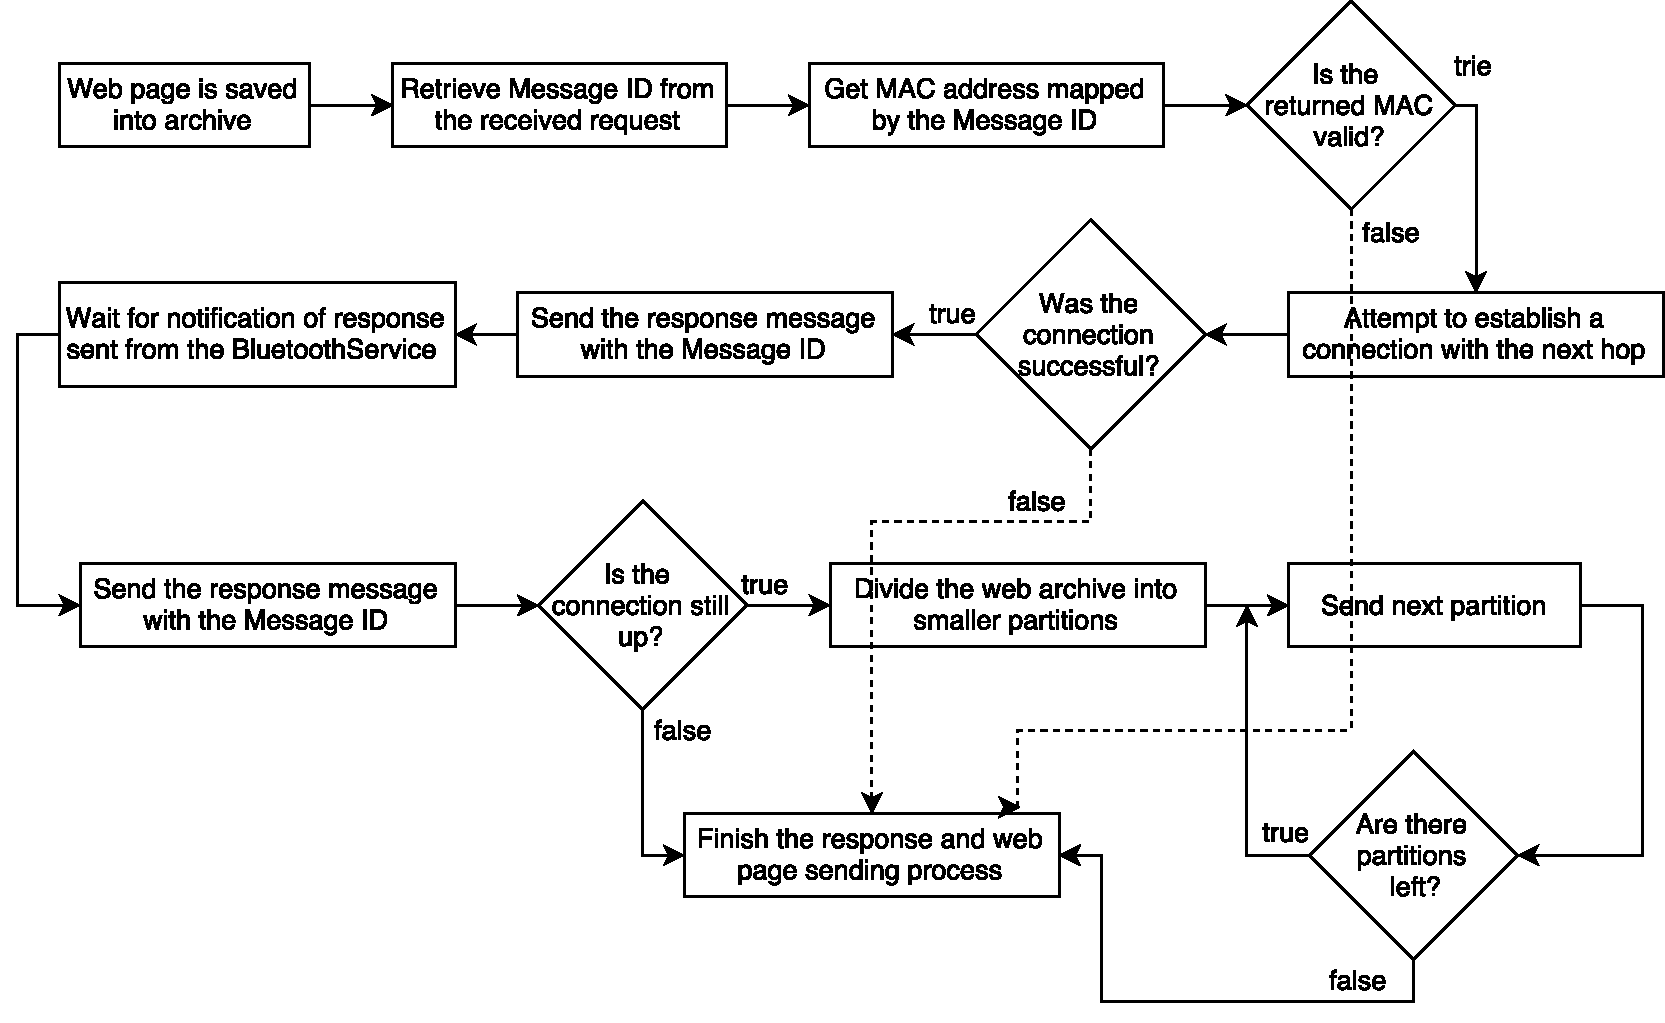
\includegraphics[width=1\textwidth]{images/send_rsp_flux.pdf}}
	\caption{\label{fig:rspsendflux} Fluxogram of the response and web page sending process}
\end{figure}

In Figure \ref{fig:rspsendflux} a fluxogram of the response sending response is presented. It shows the process from the saving of the web page to the sending of the same. As previously described the fluxogram ends by dropping the message if there is no valid next hop for that message identifier, by restarting the \textit{BluetoothService} if the connection fails, or by sending the full web page as expected.

\subsubsection{Receiving a Response Message and Web Page}
\label{subsubsec:rcvrsp}

In the receiver side, the web page and response are received and the device must assess if it is the final destination or if it is a relay node for a different device, in which case the web page will not be displayed, but the response and web page are forwarded.

This process begins in the \textit{Handler}, where the notification is notified that a message as been received by a \textit{MESSAGE\_READ}. The received message is compared with the possible types and, since it is a response message, it is identified as such. In the case of a response, the \textit{BluetoothService} is not restarted, since the device benefit from keeping the connection active to avoid further delays in re-connecting to receive the web page, also mentioned in Subsection \ref{subsubsec:sendrsp}. Instead, the \textit{BluetoothService}'s variable \textit{fileReady} is set to "true", meaning the device is has received a response message and is ready to receive the associated web page.

The message is then sent to method \textit{analyzeMessage} as a \textit{String}, where the message identifier will be saved to \textit{msgID}, retrieved from the response message, see Figure \ref{fig:rspmsg}. Having the message identifier the method compares the device's \gls{MAC} address to the one returned from \textit{getRspHop()} for that same message identifier. If both addresses match the device is the destination and the owner of the request, so the web page will be displayed. Otherwise, the response will be forwarded to the next destination.

The sender will then proceed to transfer the web page bytes from one device to another. At this point the receiver is expecting a file, since the variable \textit{fileReady} is set to "true". This shifts the \textit{BluetoothService} reception logic from receiving a \textit{String} to receiving a web page, see Subsection \ref{subsubsec:connected} for more details on this logic.

A variable \textit{output} is created, where each 990 bytes chunk is saved. When the transfer reaches the last chunk, identified by its size, which will be smaller than 990 bytes, the information contained in this variable is passed to a byte array, that will be sent back to main activity via a \textit{FILE\_READ Message}.

Once the main activity's \textit{Handler} receives this notification it copies the bytes received from \textit{BluetoothService} to a file in the application's directory. The \textit{BluetoothService} is restarted and the variable \textit{fileReady} is set to "false", as the device does not expect to receive anymore files for the time being. A new comparison between the device's own \gls{MAC} and the result of \textit{getRspHop} for that specific message identifier is made. If the result is false, meaning the device is not the destination, the response is forwarded through \textit{sendResponse}, with the corresponding message identifier, see \ref{subsubsec:sendrsp} for information on this process.

However, if the device is deemed the owner of the original request and thus the destination of the web page, the method \textit{loadPage()} is called, were the logic to display the web page is performed. First the \textit{WebView} instance is set to load web pages first from cache instead of directly trying to access the network, via \textit{setCacheMode(WebSettings.LOAD\_CACHE\_ELSE\_NETWORK)}, see \cite{webview} for more documentation. It is followed by setting the \textit{WebView}'s visibility to \textit{VISIBLE}.


There is one important aspect of this application that was not yet discussed. When the requester receives the web page, it might be needed to request multiple pages, for instance in a Google search, the user requests the front page and then inserts its query and a subsequent page is requested. This logic has to be reflected in the application for it to be deemed useful and usable. If the user had to go back and input each \gls{URL} by itself the application would have no real application.

\textit{WebViewClient}'s class may have a solution to this problem. The class method \textit{onReceivedError} is triggered whenever the \textit{WebView} receives an error, meaning it is possible that, whenever a "no Internet" error is received logic can be created in order to prevent the \textit{WebView} to display that error and instead create a request with the \gls{URL} that returned the error.

To do that, this method is overwritten, beginning by loading the page "about:blank", a page composed of a white screen, in order to avoid the user seeing the error page. A request message is then sent, via \textit{sendRequest} with the arguments: "true", -1 and the \gls{URL} that originated the error, see \ref{subsubsec:sendrqt} for a reminder on how this process is carried. Alongside this, a new \textit{WebChromeClient} is assigned, to handle the display of the web page, see \cite{webview} for more information on this class.

Finally, the web page is displayed via the \textit{WebView} method \textit{loadURL}, which for Android versions superior to 5.1 works perfectly. However if the device's Android version is prior to that the archive where the web page is saved has a different formatting and, as such, needs to be compiled again, via \textit{loadArchive()} by calling \textit{WebView}'s method \textit{loadDataWithBaseURL()} with data retrieved from the saved archive with the methods \textit{getStringFromFile()} and \textit{convertStreamToString()}, taken from \cite{stack}.

\begin{figure}[ht]
   \noindent\makebox[\textwidth]
    {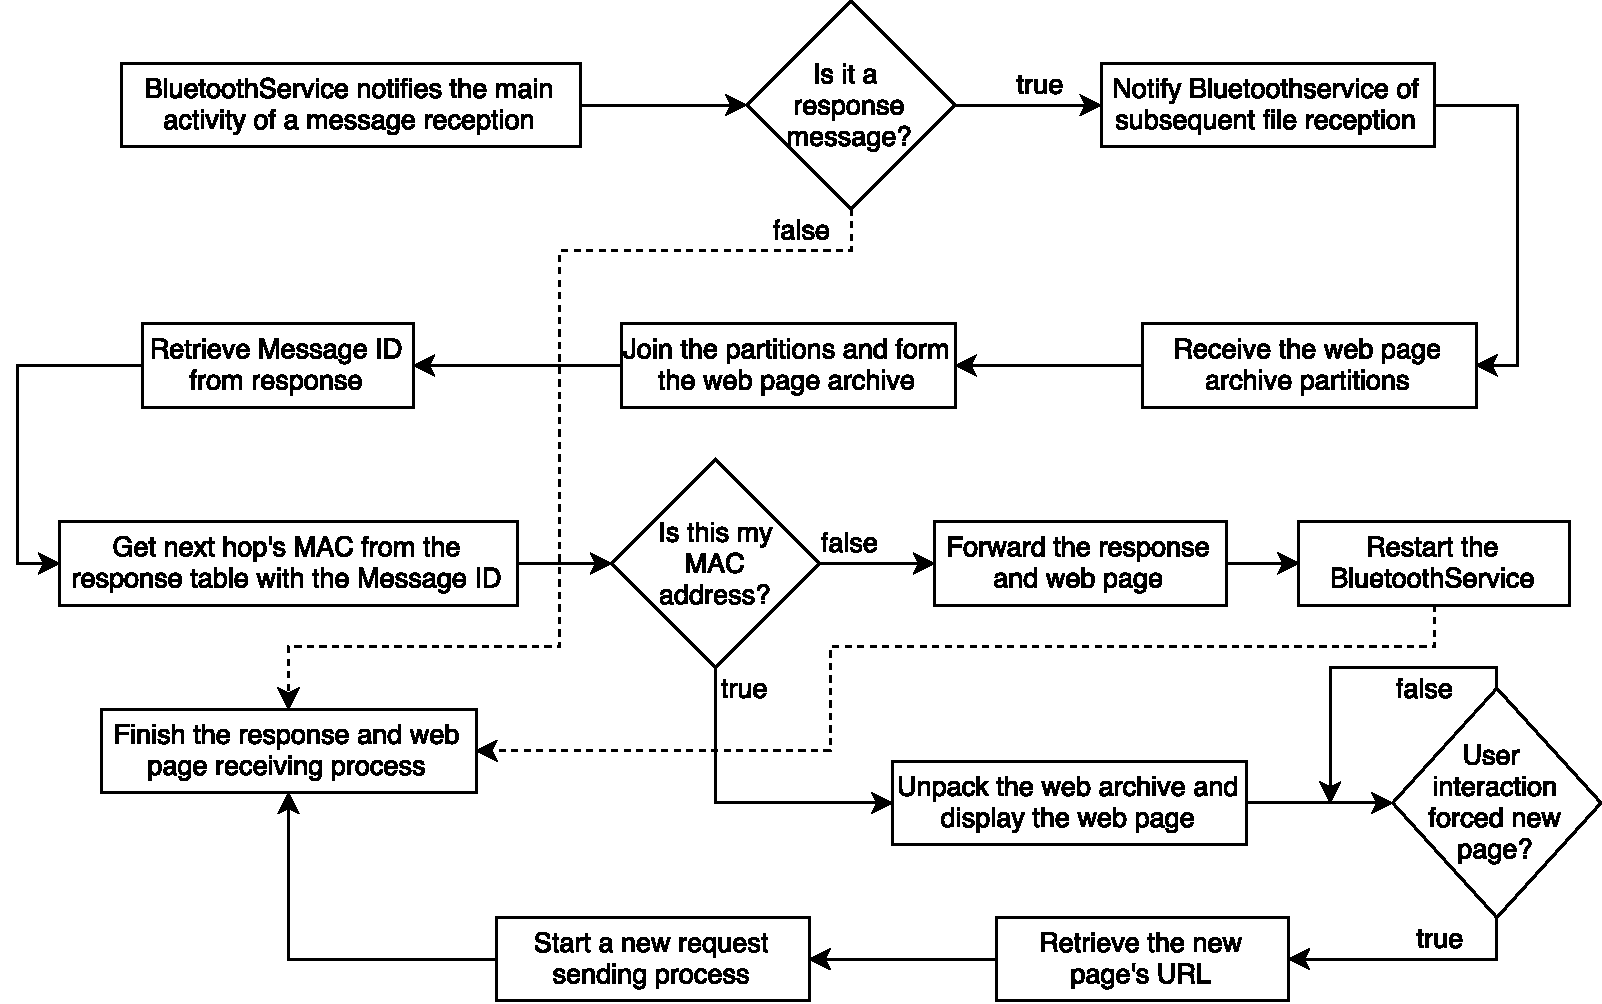
\includegraphics[width=1\textwidth]{images/rcv_rsp_flux.pdf}}
	\caption{\label{fig:rsprcvflux} Fluxogram of the response and web page receiving process}
\end{figure}

In Figure \ref{fig:rsprcvflux} a simplified fluxogram of the response and web page receiving process is shown. It is possible to visualize the file receiving logic, as well as the different possibilities for the receiver of the response: forwarding the response or displaying the web page. It is also shown the logic behind the multi web pages request.

With this implementation the user is capable of seeing the request web pages and navigate through those pages without having to manually send each request.

To finalize the example from Figures \ref{fig:example1.0} and \ref{fig:example1.1}, device C, after finishing the download of the web page, will check its response table and send a response message to device B, which is the next hop retrieved for that specific message identifier \textit{MsgID \#1}. The response is followed by the web page archive, previously downloaded, as described in Subsection \ref{subsubsec:sendrsp}.

Device B receives the response and the web page following the steps previously explained in Subsection \ref{subsubsec:rcvrsp} and checks its response table for that message identifier. Device A's \gls{MAC} is returned from that query and that's the destination for B's response, so device B sends the response and web page to A.

A receives the response and web page following the same steps as B. However, when checking the next hop for that message identifier device A gets its own \gls{MAC} address and concludes it is the final destination for that response, proceeding to display the web page requested by the user, as described this subsection.

\begin{figure}[ht]
   \noindent\makebox[\textwidth]
    {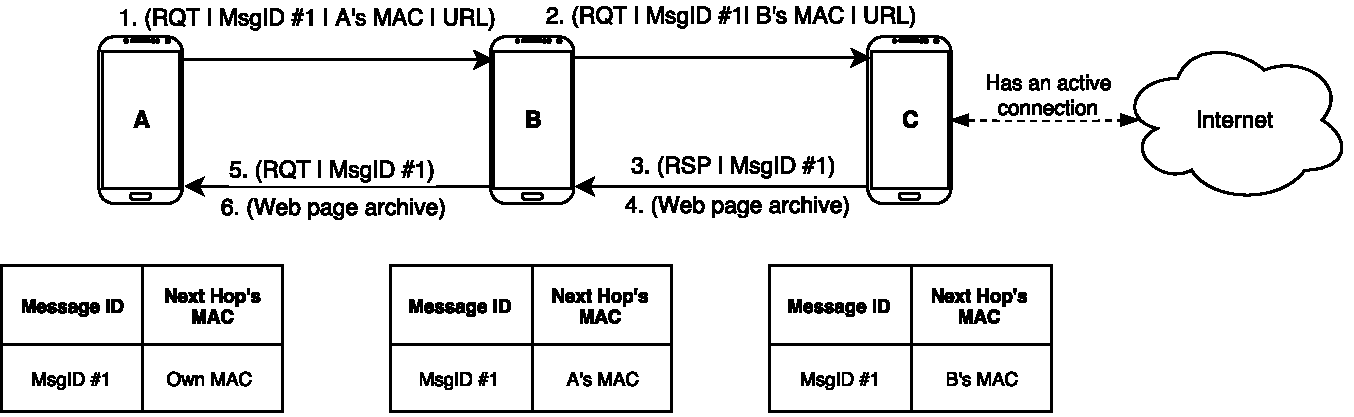
\includegraphics[width=1\textwidth]{images/example_1_2.pdf}}
	\caption{\label{fig:example1.2} Example 2: Sending and receiving of response messages and web pages}
\end{figure}

Figure \ref{fig:example1.2} illustrates this example and messages exchanged between the three devices, as well as the response tables, previously established in Figure \ref{fig:example1.1}.












\chapter{Tests and Results}
\label{tests}

In this chapter several experiments will be performed in order to assess the quality and features of technologies and developed application. The main goals are to obtain an empiric and realistic conclusion on which technology serves better the purpose of this thesis and to assess how the application fares when subject to different stress tests.

This chapter will be divided in two different sections: one regarding the comparison between Bluetooth and Wi-Fi Direct via different tests and other regarding the tests performed with the developed application, to better understand where it performs better and worse, proving or not if the theoretical choices made translate into actual performance gains.

\section{Bluetooth vs. Wi-Fi Direct}

This section will cover the differences, advantages and disadvantages of both Bluetooth and Wi-Fi Direct. A series of experiments will be conducted and their results analysed, providing a justification on which technology is best suited for this application and applications with a similar architecture and/or purpose.

Since the first implementation of Bluetooth in Android several releases have been developed. Different Bluetooth versions provide different \gls{QoS}, this may impact the performed tests as a device running a newer Bluetooth version may provide better results than a device running an older version. To avoid confusion all the tested devices will be running Bluetooth version 4.0.

The tests will range from battery consumptions to data rates analysis and most of them will be backed up by both theoretical and empirical results, although in some of them, due to the inability of getting precise measures, the results will be taken from previous developed works.

\subsection{Ranges of communication}

The ranges of communication of both technologies are of extreme importance. They can reduce or increase greatly the number of hops a packet has to pass through, in order to reach the destination. If the range of communication is too short, the number of connections made will increase, this may cause an overload of the network, and the deterioration of the communication medium. On the other hand, if the communication range is long the devices are able to jump through bigger hops, creating less traffic in the network and establishing the least possible number of connections.

Both technologies share some similarities, they are both dependent on the environment of the communication, the elements that are surrounding the devices and possible obstacles in the way. The experiments were conducted, for the obstacle experiment, in a corridor of Torre Norte in the vicinities of Instituto Superior Técnico and, for the line of sight experiment in the outside area of the same. It is important to note that although this experiments were made with as little interference as possible, there are certain elements that are impossible to controls, such as wireless communications from other devices, metal objects, such as metal lockers and cars.

Bluetooth establishes four different classes for the devices that may use this technology, depending on the transmitting power. Mobile phones are inserted in class 2 and, for that class, the specified average range of transmission in order to have a reliable connection is 10 meters, from \cite{bluetooth}.

Wi-Fi Direct on the other hand offers, theoretically, ranges of communication up to, approximately, 200 meters, from \cite{wfdrange}, which poses for a much better solution, in terms of network off-loading and general depth.

In order to verify these claims from both technologies, two mobile devices were taken to an open space, although with some limitations as described above, and several searches were made, until the devices stopped being discovered by one another. After measuring the distance between both devices, the results were taken, and prove what was already to be expected, although with some twists. 

Bluetooth was able to create a connection between devices from a distance up to 42 meters apart, see Figure \ref{fig:btMaxVisib} for the overall scheme of this experiment. This value is a lot more than what was expected judging by the theoretical value of 10 meters, although the health of the connection was not verified, see \ref{subsec:ftdr} for these tests. Using Wi-Fi Direct the devices were able to communicate from a maximum distance of 77 meters, see Figure \ref{fig:wfdMaxVisib} for the overall scheme of this experiment, which is, considerably, smaller than the theoretical value of 200 meters.

\begin{figure}[ht]
   \noindent\makebox[\textwidth]
    {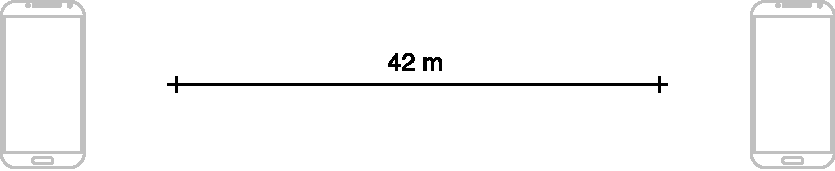
\includegraphics[width=0.8\textwidth]{images/bt_max_visib.pdf}}
	\caption{\label{fig:btMaxVisib} Max range of Bluetooth communication with line of sight between devices}
\end{figure}

\begin{figure}[ht]
   \noindent\makebox[\textwidth]
    {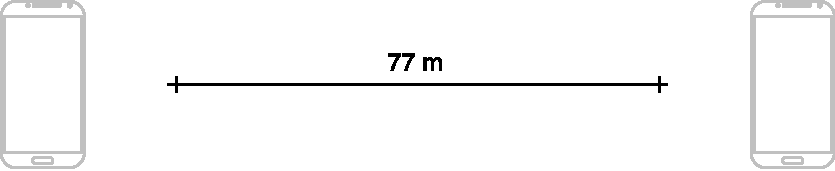
\includegraphics[width=0.8\textwidth]{images/wfd_max_visib.pdf}}
	\caption{\label{fig:wfdMaxVisib} Max range of Wi-Fi Direct communication with line of sight between devices}
\end{figure}

Both tests were made with a direct line of sight between devices. For the next ones there will be obstacles in the way of communication. It is expected that this affects greatly the communication ranges. The first test was made using Bluetooth technology where a wall was blocking the line of sight between devices, see Figure \ref{fig:btMaxInv}. The second test was made using Wi-Fi Direct, and, in order to maintain the same environment as the previous experiment, to get reliable results, it was situated in the same place as the first, see Figure \ref{fig:wfdMaxInv}. However, due to the environment configuration, it was impossible to recreate the experiment with only one wall, so two walls are now dividing the devices. Since the walls introduce a loss in the signal power, the more walls are between devices, the bigger the losses will be.

\begin{figure}[ht]
   \noindent\makebox[\textwidth]
    {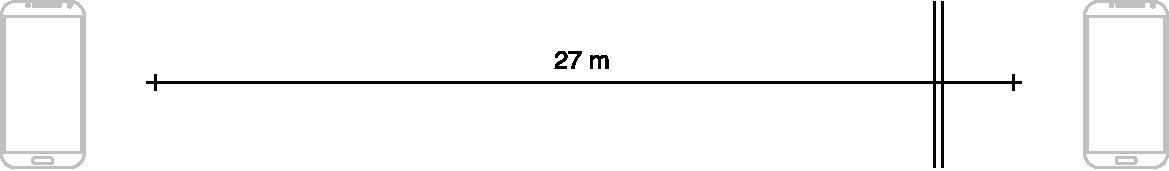
\includegraphics[width=0.8\textwidth]{images/bt_max_inv.pdf}}
	\caption{\label{fig:btMaxInv} Max range of Bluetooth communication without line of sight between devices}
\end{figure}

\begin{figure}[ht]
   \noindent\makebox[\textwidth]
    {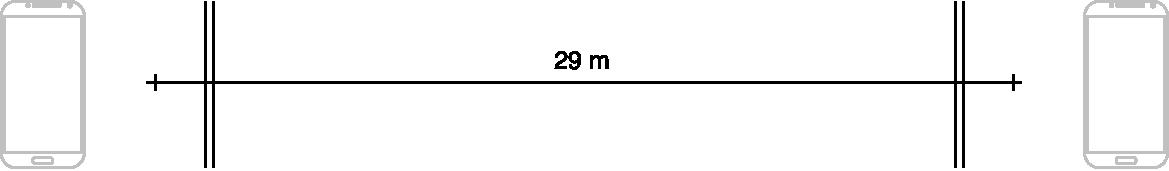
\includegraphics[width=0.8\textwidth]{images/wfd_max_inv.pdf}}
	\caption{\label{fig:wfdMaxInv} Max range of Wi-Fi Direct communication without line of sight between devices}
\end{figure}

As expected the obstacle, in this case the wall, created a significant decrease on the maximum range of communication. Bluetooth was able to communicate from a distance of 27m, closer to the theoretical 10 meters.

Wi-Fi Direct was also able to communicate from a smaller maximum distance, measuring 29 meters, with the signal passing through both walls. From a smaller distance it was verified that this technology could communicate with only wall in the way, meaning it also surpasses Bluetooth when an obstacle is in the way of communication.

After these experiments it is possible to conclude that Wi-Fi Direct is more desirable, since it provides better coverage than Bluetooth to similar areas. Also, there is no evidence that Wi-Fi Direct suffers more losses from obstacles, maintaining its desirability. This was already to expect, both from the theoretical values and from the transmission powers\footnote{Transmission powers impact directly the range of transmission, since they affect the signal strength, a crucial characteristic for receivers to better capture the transmissions. A bigger transmit power, usually, creates a bigger signal strength leading to the signal being capture over bigger distances, as referred in \cite{txpower}, for instance.}, since Bluetooth is mostly known for its lower transmit powers, if compared to technologies such as Wi-Fi.

\subsection{Battery consumptions}

\subsection{Discovery times}

The discovery time is a critical factor for this work. The discovery process is the one of the bigger time consumers during an application run. Thus, minimizing it, is a great advantage for the overall performance of the application.

For the purpose of testing the Bluetooth and Wi-Fi Direct discovery times, three mobile devices where used: Samsung Grand Neo, running Android version 4.2.2; Motorola Moto G2, running Android version 7.1; Huawei P8 Lite, running Android version 6.0, providing an heterogeneous sample space.

Bluetooth version 4.0 theoretically provides a discovery time of 10.24ms, as mentioned in \cite{btdisc1} and \cite{btdisc2}, and, to confirm this hypothesis, discovery times values from the three devices were measured. Each device was submitted to multiple discoveries with a different number of discovered peers, ranging from 0 devices found to 3 devices found.





\subsection{File transfer data rates}
\label{subsec:ftdr}

\section{Testing the developed application}

\subsection{Battery consumption during use}

\subsection{Discovery times}

\subsection{Connection times}

\subsection{File transfer data rates}





%!TEX root = ../dissertation.tex

\chapter{Conclusions}
\label{chapter:conclusion}

In this chapter the conclusions of the developed work will be stated. It is divided into two sections: the first one will provide a brief summary on what was accomplished with this work. The second, regarding the limitations and possible future work of the developed framework and application.

\section{Summary}

In Chapter \ref{chapter:soa}, a theoretical description of the most common cellular communication technologies was presented. Moreover, Bluetooth and Wi-Fi Direct's Android implementations were analysed, in order to provide an overview of how were these technologies used to achieve ad hoc networks and multi-hop routing within them. This analysis establishes the rough guidelines on which the developed framework would be based.

The developed framework accomplishes everything that was stated in Section \ref{sec:objectives}. A decentralized ad hoc network can be successfully established, using mobile devices with unmodified Android system versions. Moreover, although the framework was developed using the Bluetooth technology, it is easily adaptable to other communication technologies. This is achieved due to the division of protocol/communication technology present in the framework, as can be seen in Figure \ref{fig:appsandbox}. By creating the necessary links between the protocol and the communication technology, the framework is easily updated to use a different communication technology, such as Wi-Fi Direct.

The developed application also accomplishes the goals set in Section \ref{sec:objectives}. A mechanism to download, store, transfer and display web pages was implemented. The developed application functions as intended, providing a simple but seamless web browsing experience to the user and, allowing the relay and Internet Access Point nodes to be running the application in background.  Moreover, with a few tweaks, the developed application can be adapted to transfer different data formats, such as pictures, videos, or even simple messages. To accomplish this, it is needed to modify the data download and display mechanisms, adjusting them to whatever format is chosen, the remaining mechanisms can remain unchanged, as they are common to every format type.

The second objective of this thesis was to assess the advantages of Wi-Fi Direct over Bluetooth, and what the next Android system versions should be modifying to provide a meaningful Wi-Fi Direct impact, in peer-to-peer applications. This objective was fulfilled in Sections \ref{sec:btvswifi} and \ref{sec:btvswifitests}, where a set of study tests were performed, in order to show Wi-Fi Direct's advantages over Bluetooth.

The developed application was subject to a set of tests, aiming to assess its performance during the different processes it executes when running. The results show that the application fares the worse during the discovery process. The advertisement process suggests a linear scaling with the number of advertised peer devices. The web page exchange process throughput was smaller than the native Android's Bluetooth throughput, but this was to be expected since other delays are introduced during this processed.

Overall, the application's performance could be increased by introducing Wi-Fi Direct as the communication technology and by transitioning the discovery and advertisement processes to a beacon advertisement and search mechanism, such as the one provided by \gls{BLE}.

After the research and testing performed, it is possible to state that Wi-Fi Direct should provide an Android implementation improvement. This improvement must address the issue of user interaction when connecting two devices. If this feature is officially provided by Android, more and more applications can use Wi-Fi Direct as an alternative to Bluetooth, in Android peer-to-peer applications. Moreover, \gls{BLE}'s current Android implementation should also be improved, allowing Android devices to transmit and receive beacon advertisements.

\section{Future Work}
\label{sec:futurework}

The developed framework and application accomplish the basic functions, \textit{i.e.}, the foundation, required for a market-ready solution. However, they both have some limitations. In this section, these limitations will be analysed, explaining how future work on the developed items can tackle the current limitations.

Starting by the developed framework, it provides a easy to use set of methods with the purpose of establishing an ad hoc network. Its main limitations are the following:

\begin{itemize}
	\item The used technology is Bluetooth, known for its low energy consumption. A better choice for the developed framework would be Wi-Fi Direct, providing (1) a larger range of communication, expanding the network reach; (2) faster data rates, reducing the time of message exchanges and overall application runtimes. Although this technology provides some advantages over Bluetooth, its current Android implementation does not allow the transmission of data without user intervention, invalidating its use in most applications.
	
	\item The implemented routing protocol is simple and light, providing an excellent solution for time sensitive applications. However, it does not support alternative path finding and data retransmission, in case of failure. In Subsection \ref{subsec:routprot}, a possible routing protocol is proposed, that despite being heavier, for reasons mentioned before, provides a robust solution to transmission and path failures.
	
	\item The discovery and advertisement process is slow and could be improved by using \gls{BLE}'s beacon technology. Devices would periodically send a beacon message, allowing peer devices to capture and store that information. This mechanism would be much more efficient than creating individual connections with each peer device to transmit the Advertisement message. However, although the used devices\footnote{List of devices supporting \gls{BLE}'s beacon advertisement: \url{http://altbeacon.github.io/android-beacon-library/beacon-transmitter-devices.html}.} support \gls{BLE}, its current Android implementation only allows devices to capture the beacon messages, not to send them, thus invalidating the development of this mechanism.
	
	\item In this framework, security is not implemented. Despite that, it is possible to provide a rough overview of how a secure framework could be achieved (1) a central hub would be created, where Internet connected devices would send the requests; (2) a public/private key mechanism would be implemented, where every device, using an application with the developed framework, would be given the central hub's public key; (3) once a device opened the application, it would encrypt its public key with the central hub's public key, creating a sort of register mechanism; (4) all subsequent sent requests would be encrypted using the central hub's public key; (5) upon receiving a request, the central hub would decrypt the message using its private key. It would then proceed to encrypt the response data with the public key of the request originator, received in the registration process; (6) upon receiving a response to a originated request, it would be decrypted, using the device's private key.
	
	With this security mechanism, the messages would be safely transferred between devices, without the possibility of a device decrypting data of a request it didn't originate. Furthermore, to improve the central hub's security, every stored response and request would be encrypted with a safe, well-known encryption algorithm, \textit{e.g.} \gls{AES}-256. The central hub's storage system and overall structure is still open to debate, and could provide an interesting work to research and develop, hereafter.
	
\end{itemize}

The developed application provides a solid mechanism to provide web access to devices without Internet connection. Its main limitation resides in the capture and transmission of the web pages:

\begin{itemize}
	
	\item The mechanism used to store the web pages is to retrieve a web page archive. This archive stores the web page in a single file, easily uncompressed and displayed. Although this appears to be the perfect solution for the web page storage, it has some flaws, inherent to the method used to retrieve the archive, \textit{savewebarchive()}. This method's last major update was in October, 2013, with the introduction of Android API level 19 (see \cite{kitkat}) and, since then, web pages have suffered lots of improvements. Some of the new web page features may not be stored, due to the method's lack of compatibility thus, some web pages' interactive features may not be responsive.
	
	\item To successfully implement a full web browser experience, video streaming and file transfers should be possible. However, due to their implementation complexity, these features were left out of the initial development. These features would provide a challenging future work in this thesis, as they would include image, sound and file encryption and compression.
	
\end{itemize}



\bibliographystyle{ieeetr}
\addcontentsline{toc}{chapter}{Bibliography}
\bibliography{bibliography/dissertation}


% Appendix
\appendix
%!TEX root = ../dissertation.tex

% Appendix chapters entry point
% Include the chapters below

%!TEX root = ../dissertation.tex


% Glossary and Acronym List
\if\includeGlossary 1
\printglossary
\fi

\end{document}